%
%  @Coding: utf-8
%  @Description: 本科毕业设计论文主文件
%
% chktex-file 1
% chktex-file 24
% chktex-file 36
% chktex-file 44

\RequirePackage{fix-cm}
\documentclass[bachelor, print]{xduthesis}
\usepackage{graphicx}
\usepackage{subfig}
\usepackage{float}
\usepackage{array}
\usepackage{url}

\makeatletter
\pdfstringdefDisableCommands{%
    \let\xiaosi\@empty
    \let\CJKfamily\@gobble
    \let\hskip\@gobble
    \let\kern\@gobble
}
\makeatother

\newcommand{\figplaceholder}[2]{
    \begin{figure}[H]
        \centering
        \fbox{
            \begin{minipage}[c][0.28\textheight][c]{0.82\linewidth}
                \centering
                #2
            \end{minipage}
        }
        \caption{#1}
    \end{figure}
}

\begin{document}

%%%%%%%%%%%%%%%
%% 论文前置部分
%%%%%%%%%%%%%%%
\frontmatter

% 论文相关信息（封面）
\classid{2203054w}
\studentid{22009201185}
\cschool{计算机科学与技术学院}
\ctitle{智能客服机器人的设计与交互优化}
\cauthor{王奇}
\cmajor{计算机科学与技术}
\csupervisor{魏昱恒、Harris H M XIE}

% 中文摘要
\begin{cabstract}
随着银行业务线上化和智能服务渠道的发展，传统银行系统在余额查询、交易流水查询、账单统计和常见问题咨询等高频场景中，仍存在页面路径较长、筛选条件复杂、静态 FAQ 难以处理实时业务数据等问题。同时，银行业务涉及账户余额、交易流水和资金转账等敏感信息，若直接依赖大语言模型生成业务事实或执行资金操作，容易带来结果不可控和误操作风险。针对上述问题，本文设计并实现了面向个人银行业务的智能客服机器人原型系统 BankCopilot。系统采用 Vue 3、Element Plus、ECharts、Spring Boot、MyBatis 和 MySQL 构建前后端业务能力，并接入通义千问大模型完成自然语言意图解析与分析性文本生成。本文提出“大模型理解与表达、后端确定性服务提供业务事实和执行控制”的系统设计思路：大模型负责将用户输入解析为余额查询、流水查询、账单统计、FAQ 咨询或转账等结构化意图，账户数据、流水数据、统计结果和转账执行均由后端服务和数据库完成。系统实现了文本与语音转文字输入、AI 查余额、AI 查流水、AI 账单统计与分析、AI 周报/月报、FAQ 知识库问答、异常情绪安抚、人工客服引导和 AI 智能转账二次确认等功能，并通过 SSE 流式响应、处理过程展示、统计图表、快捷操作和导出链接优化交互体验。测试结果表明，系统 21 项后端自动化测试全部通过；80 条意图与分流测试样本通过率为 95.0\%；FAQ 知识库能够对银行相关问题返回标准答案或相似推荐，并对无关问题进入未命中分支；9 名匿名测试者在本地原型和虚拟演示业务数据环境下形成 81 条真实任务聊天记录，核心任务均能完成。结果说明，BankCopilot 能够在保持银行业务数据可追溯和资金操作可确认的前提下，缩短高频业务查询路径，补充常见问题分流能力，并提升智能客服交互的可解释性和可控性。
\end{cabstract}

\begin{ckeywords}
智能客服机器人\quad 大语言模型\quad 自然语言处理\quad 银行业务\quad 账单分析\quad 交互优化\quad 二次确认
\end{ckeywords}

% 英文摘要
\begin{eabstract}
With the development of online banking services and intelligent service channels, traditional banking systems still have long operation paths, complex filtering conditions, and limited static FAQ support in high-frequency scenarios such as balance inquiry, transaction inquiry, bill statistics, and common service consultation. Meanwhile, banking services involve sensitive information such as account balances, transaction records, and fund transfers. If a large language model is allowed to directly generate business facts or execute fund operations, the system may suffer from uncontrollable results and mistaken operations. To address these problems, this thesis designs and implements BankCopilot, an intelligent customer service robot prototype for personal banking services. The system uses Vue 3, Element Plus, ECharts, Spring Boot, MyBatis, and MySQL to build front-end and back-end business capabilities, and integrates the Qwen large language model for natural language intent parsing and analytical response generation. This thesis adopts the design principle that the large language model is responsible for understanding and expression, while deterministic back-end services provide business facts and execution control. The model parses user input into structured intents such as balance inquiry, transaction inquiry, bill statistics, FAQ consultation, or transfer, whereas account data, transaction data, statistical results, and transfer execution are all handled by back-end services and the database. The system implements text and speech-to-text input, AI-based balance inquiry, transaction inquiry, bill statistics and analysis, weekly or monthly brief generation, FAQ knowledge-base question answering, emotional support, human service guidance, and two-step confirmation for intelligent transfer. It also improves interaction through SSE streaming responses, process tracing, statistical charts, quick actions, and export links. The test results show that all 21 back-end automated tests passed; the pass rate of 80 intent and routing test samples reached 95.0\%; the FAQ knowledge base could return standard answers or similar recommendations for banking-related questions and route irrelevant questions to the no-answer branch; nine anonymous testers generated 81 real task chat records in the local prototype environment with virtual demonstration business data, and the core tasks were completed. The results indicate that BankCopilot can shorten high-frequency business inquiry paths, supplement common-question routing, and improve the explainability and controllability of intelligent customer service while keeping banking data traceable and fund operations confirmable.
\end{eabstract}

\begin{ekeywords}
intelligent customer service robot\quad large language model\quad natural language processing\quad banking service\quad bill analysis\quad interaction optimization\quad two-step confirmation
\end{ekeywords}

% 生成论文的封面、声明页、中英文摘要
\makecover

% 论文目录
\tableofcontents

%%%%%%%%%%%%%%%
%% 论文正文
%%%%%%%%%%%%%%%
\mainmatter

\chapter{绪论}

\section{研究背景与问题提出}

在数字化服务持续发展的背景下，银行业务从传统柜台办理逐步转向移动端、网页端和智能终端。用户在办理业务时，常常需要查询余额、查询交易流水、了解一段时间内的收支状况，或者发起转账等操作。这些需求频率高、重复性强，若完全依赖人工客服，不仅会增加银行服务成本，也会影响用户问题响应速度。因此，构建能够理解自然语言、连接业务系统并提供即时服务的智能客服机器人，具有较强的工程意义和应用价值。

近年来，大语言模型在自然语言理解和文本生成方面表现出显著能力，使客服机器人从传统的基于规则或检索的问答系统逐步发展为能够处理开放式表达和多轮上下文对话的智能助手\cite{zhao2023survey}。但在银行场景中，单纯依赖大模型直接回答并不可靠。银行业务涉及账户余额、交易流水和资金转账等敏感数据，要求系统具备准确性、可审计性和安全性。因此，本课题将大语言模型作为自然语言入口和表达增强工具，将真实业务查询、统计计算和资金操作交由后端确定性服务完成，从而在智能化体验和业务安全之间取得平衡。

BankCopilot 项目以银行智能客服为场景，实现了一个面向个人账户业务的 AI 助手。为避免后文概念混用，本文将“客服机器人”“智能客服助手”“AI 助手”等表述统一指向 BankCopilot 智能客服机器人；其中“AI 助手”主要用于描述前端聊天入口和交互界面。系统支持用户使用文本自然语言或语音转文字方式发起查询与操作请求，能够完成余额查询、流水查询、账单统计、周报/月报生成以及智能转账确认等功能。与普通客服问答系统相比，本系统的特点在于 AI 回复并非仅来自静态问答库，而是通过意图解析后调用真实账户、流水和统计服务，再将结果组织为用户可理解的文本、图表和报表导出链接。

从银行业务应用角度看，智能客服机器人并不只是一个问答窗口，而是业务入口、交互流程和风险控制逻辑的组合。用户在传统页面中完成一次流水查询，通常需要进入交易流水页面、选择交易类型、设置起止日期、调整分页参数，再阅读表格结果；而在智能客服交互中，用户可以直接表达“查最近 5 条支出记录”或“看最近 7 天支出趋势”。系统需要将这类口语化表达转换为后端能够执行的查询条件。该转换过程既涉及自然语言理解，也涉及业务规则约束。若只关注文本生成能力而忽略业务执行过程，智能客服就容易停留在演示层面，难以成为真正可用的银行服务入口。

另一方面，银行业务对准确性和安全性要求较高。余额、流水和转账结果均属于用户关心的敏感信息，系统不能让模型根据语言习惯自行推断或编造金额。本文的设计思路是将大模型放在“理解用户意图”和“组织分析语言”的位置，将数据库查询、统计聚合和资金变动放在传统后端服务中执行。这样既可以利用大模型提升自然语言交互的灵活性，又可以通过确定性服务保证数据来源可追溯、业务流程可控制。该思路也是本文相对于简单聊天机器人实现的主要区别。

结合银行智能客服的业务特点，本文将课题问题进一步细化为四个方面：第一，传统银行业务页面依赖菜单、表单和筛选条件，用户完成余额查询、流水筛选和账单统计等高频操作时路径较长；第二，普通 FAQ 问答只能处理固定咨询，难以连接账户、流水和统计等实时业务数据；第三，大语言模型虽然具备自然语言理解和表达能力，但不能直接作为余额、流水、统计金额和转账结果的事实来源；第四，转账等资金类操作具有较高风险，智能客服必须在参数解析、后端校验和用户确认之间建立清晰边界。因此，本文研究的核心问题不是简单构建一个聊天机器人，而是在银行业务原型系统中设计一种可解释、可控制、可验证的 AI 辅助交互流程。

\begin{figure}[H]
    \centering
    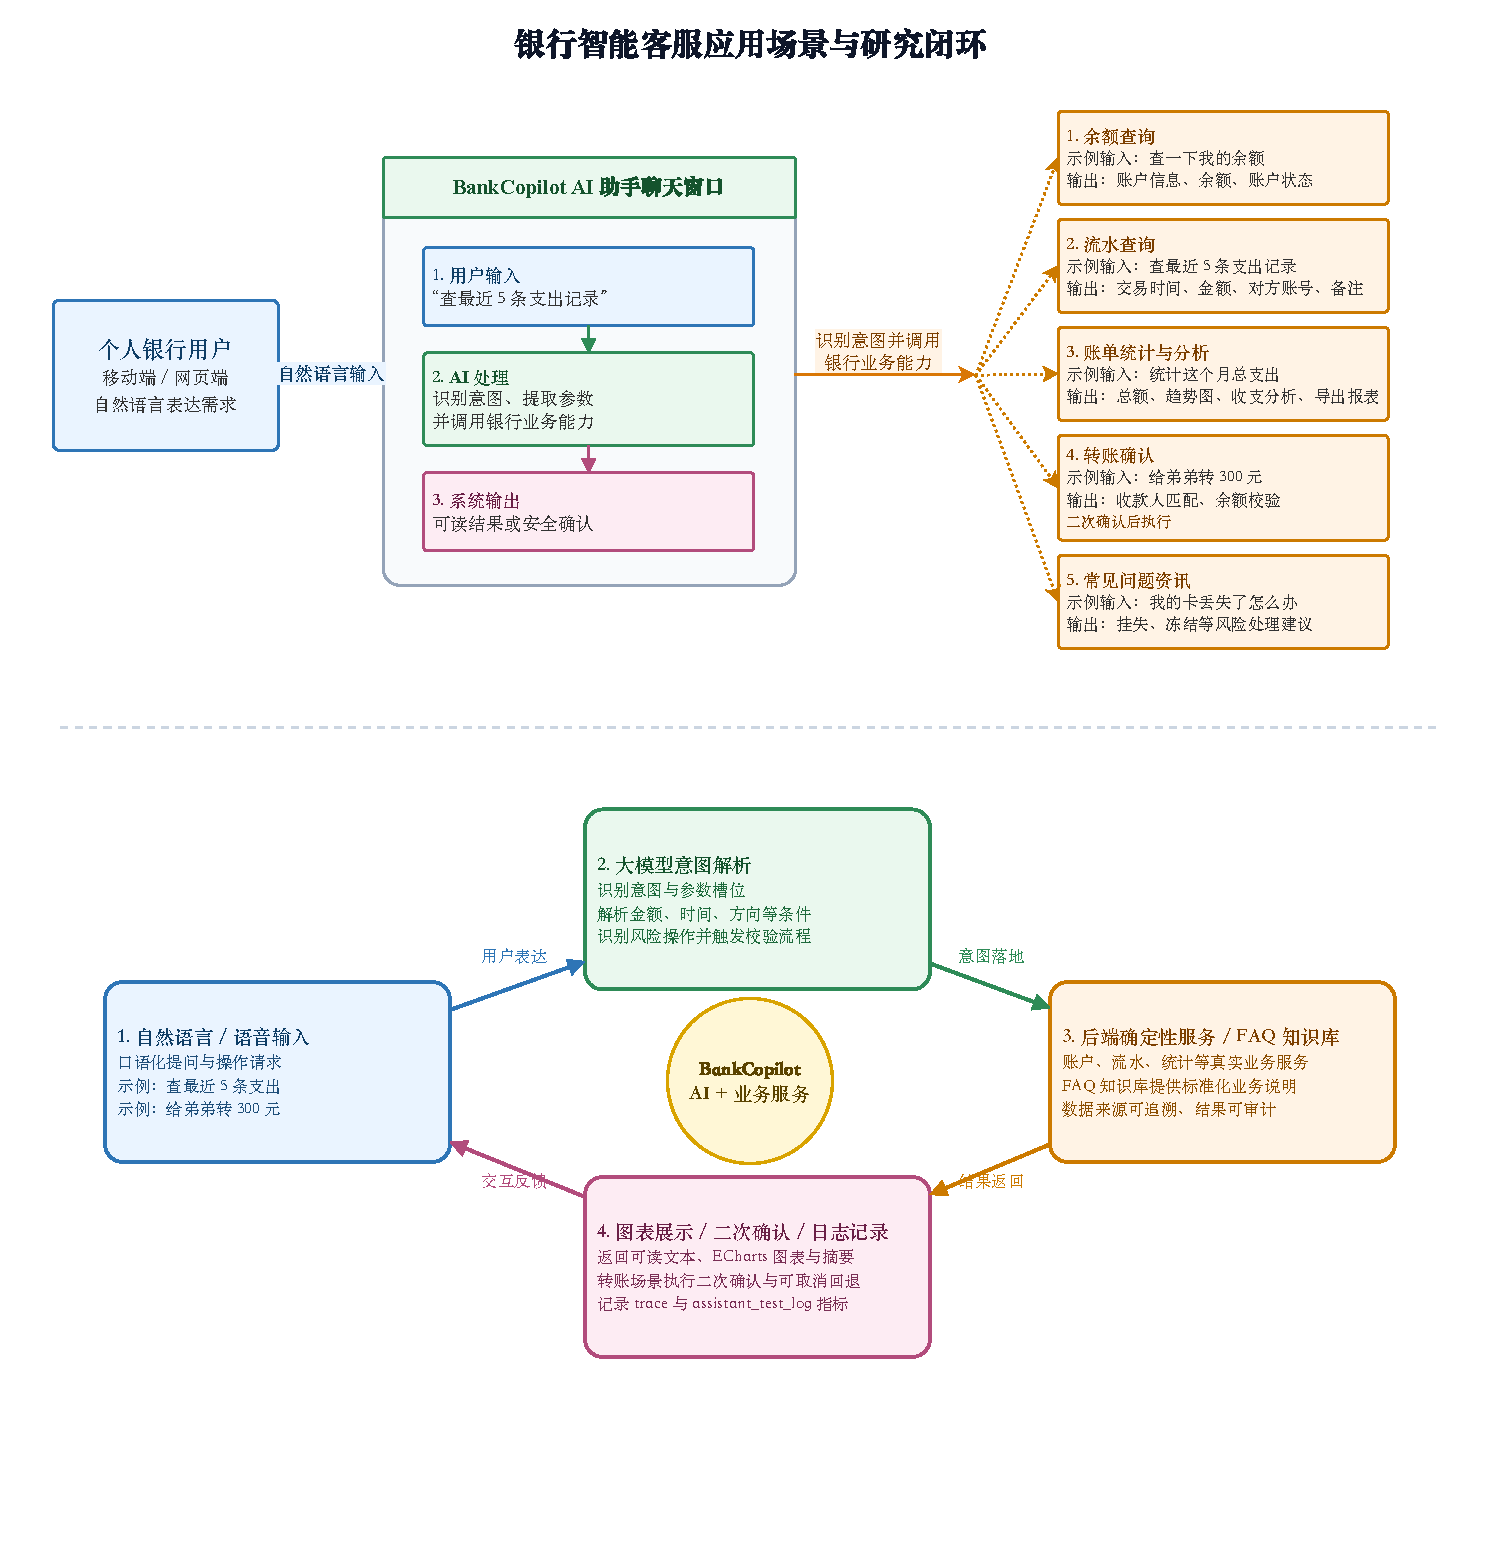
\includegraphics[width=0.92\linewidth]{image/fig-bank-ai-service-scenario-simsun.pdf}
    \caption{银行智能客服应用场景与研究闭环示意图}
\end{figure}

\section{课题目标、研究内容与创新点}

本课题的总体目标是设计并实现一个面向银行业务的智能客服机器人原型。课题重点研究自然语言交互、业务意图解析、对话状态管理、银行业务服务集成和前端交互优化等内容。系统以文本自然语言交互为主要方式，并补充语音转文字输入能力，围绕用户在个人银行业务中的高频需求提供智能化辅助。

结合任务书要求和项目源码实现，本文的主要研究内容包括以下几个方面。

第一，设计智能客服机器人的功能体系和交互流程，明确 AI 助手支持的业务边界。第二，选择适合项目的自然语言处理方案，通过通义千问大模型完成用户输入到结构化意图的转换。第三，设计对话管理机制，实现转账确认和流水查询补全等多轮交互。第四，将 AI 助手与后端账户、流水、统计和转账服务集成，实现真实业务数据驱动的智能回复。第五，优化前端交互展示，提供语音输入、流式响应、处理过程追踪、图表展示、快捷操作和报表导出等能力。

\begin{table}[H]
    \centering
    \caption{课题研究内容与系统实现对应关系}
    \label{tab:research-content}
    \begin{tabular}{|p{0.22\linewidth}|p{0.68\linewidth}|}
        \hline
        研究内容 & 本文实现方式 \\
        \hline
        自然语言理解 & 通过 QwenClient 调用通义千问，将用户输入解析为 intent 字段、时间范围、金额、收款人等结构化字段。 \\
        \hline
        对话管理 & 通过 pendingMap 和 pendingTxnQueryMap 维护待确认转账和待补全流水查询状态。 \\
        \hline
        业务系统集成 & 调用 AccountService、TransactionService、StatisticsService 和 PayeeService 完成真实业务处理。 \\
        \hline
        交互优化 & 前端 AssistantPanel 实现语音输入、SSE 流式响应、AI 过程展示、图表展示、快捷确认与导出功能。 \\
        \hline
        安全控制 & 转账前校验账户、余额和收款人信息，并要求用户二次确认。 \\
        \hline
    \end{tabular}
\end{table}

上述研究内容共同构成了系统的 AI 能力闭环。自然语言理解负责把用户原始输入转换为可执行的业务意图，对话管理负责处理缺失信息和高风险操作确认，业务系统集成负责保证返回数据来自真实数据库，交互优化负责将处理过程和业务结果以更清晰的形式展示给用户。本文后续章节围绕这一闭环展开论述，避免把 AI 功能写成脱离系统实现的概念性描述。

\begin{table}[H]
    \centering
    \caption{本文创新点与后文章节对应关系}
    \label{tab:innovation-chapter-map}
    \scriptsize
    \setlength{\tabcolsep}{2pt}
    \renewcommand{\arraystretch}{1.15}
    \begin{tabular}{|p{0.17\linewidth}|p{0.21\linewidth}|p{0.25\linewidth}|p{0.25\linewidth}|}
        \hline
        创新点或优化点 & 解决的问题 & 具体实现位置 & 验证位置 \\
        \hline
        自然语言业务入口与语音转文字输入 & 传统银行页面依赖菜单、表单和筛选条件，用户完成查询路径较长。 & 5.4 接口与交互设计；6.1 AI 请求处理总体流程；6.2 AI 语音输入功能实现。 & 7.4 功能测试 T1、T2、T11；7.5 用户体验测试 U1、U2、U5。 \\
        \hline
        大模型与后端确定性服务分工 & 大模型可能编造余额、流水、统计金额或业务结论。 & 3.1 大语言模型与自然语言意图识别；5.1 系统架构设计；5.2 AI 模块设计；6.5--6.8 查询与统计功能实现。 & 7.3 意图识别准确性测试；7.4 功能测试；7.7 测试结论。 \\
        \hline
        FAQ 知识库与查询日志 & 静态客服或纯大模型回答难以保证常见银行问题答案稳定、可维护。 & 5.3 数据库设计中的 faq\_knowledge、faq\_query\_log；6.4 FAQ 知识库问答功能实现。 & 7.4 FAQ 检索统计；附录 A.4、A.5、A.6、A.7。 \\
        \hline
        多轮对话状态管理 & 用户输入缺少月份、确认、取消等上下文时，单轮问答无法正确处理。 & 5.2 AI 模块设计；6.1 AI 请求处理总体流程；6.6 AI 查流水多轮补全；6.9 AI 智能转账。 & 7.4 功能测试 T3、T7、T8、T9。 \\
        \hline
        统计解释、图表展示与简报 & 传统流水表格需要用户自行理解和计算，统计结果不直观。 & 5.4 接口与交互设计；6.7 AI 账单统计与分析；6.8 AI 周报/月报。 & 7.4 功能测试 T4、T5、T6；7.5 用户体验测试 U6；7.6 交互优化设计分析。 \\
        \hline
        转账二次确认、账号脱敏和取消回退 & AI 直接执行资金操作存在误操作风险。 & 4.3 非功能性需求；6.9 AI 智能转账功能实现；表 6.5 安全控制设计。 & 7.4 功能测试 T7、T8、T9；7.5 用户体验测试 U7。 \\
        \hline
        过程展示、统计口径说明和能力边界控制 & 用户难以判断 AI 是否真正调用业务服务，也难以识别模型是否超出能力范围。 & 5.2 AI 模块设计；6.1 响应结构 trace/explain；6.7 统计 explain/exportUrl；7.6 交互优化设计分析。 & 7.4 功能测试 T10；7.6 交互优化设计分析；7.7 测试结论。 \\
        \hline
        匿名测试日志与反馈优化闭环 & 无实际用户反馈缺乏对改进方向 & 5.3 assistant\_test\_log 数据表；7.1--7.5 测试环境、日志说明和用户体验测试；附录 A.7。 & 7.5 用户体验测试与反馈分析；附录 A.8--A.10。 \\
        \hline
    \end{tabular}
\end{table}

表 \ref{tab:innovation-chapter-map} 将本文提出的主要创新点和交互优化措施与后文章节进行对应。可以看出，本文创新并非停留在概念层面，而是分别落实到系统架构、AI 模块、数据库设计、核心功能实现和测试验证中。第五章重点说明整体设计，第六章说明各项功能的具体实现，第七章通过意图识别、功能测试、FAQ 检索统计和匿名用户体验测试验证优化效果。

本文创新性主要体现在四个方面。第一，将智能客服从普通问答窗口扩展为银行业务自然语言入口，用户可以通过文本或语音转文字输入发起余额查询、流水筛选、账单统计、FAQ 咨询和转账确认等操作。第二，提出“大模型理解与表达、后端确定性服务提供业务事实”的分工方式，使 Qwen 大模型主要承担意图解析和分析性表达生成，账户、流水、统计和转账结果由 Spring Boot 后端与 MySQL 数据库提供。第三，面向转账等高风险业务设计可确认、可取消、可追踪的多轮操作流程，将自然语言转账拆分为参数解析、后端校验、待确认、确认执行或取消回退等阶段。第四，建立“功能测试、日志记录、用户反馈、交互优化”的验证闭环，通过 assistant\_test\_log、自动化测试、意图测试、FAQ 检索统计和匿名用户体验测试补充系统效果证据。上述创新属于面向银行业务场景的系统设计和工程集成创新，而不是声称提出新的底层算法。

课题研究范围需要明确边界。系统中的登录、注册、账户验证等能力属于基础设施，不作为本文 AI 核心功能的重点，故不在本课题研究范围内。本文重点分析源码中已实现的语音输入、FAQ 知识库问答、异常情绪安抚、AI 查余额、AI 查流水、AI 账单统计与分析、AI 周报/月报和 AI 智能转账功能等 AI 集成特色功能。对于当前源码没有实现的消费品类识别、商户标签分析等能力，由于实现过于复杂且与 AI 集成不可控，仅在不足与展望中作为后续方向说明。

\section{本文组织结构}

本文共分为九章。第一章介绍课题背景、问题提出、研究目标、研究内容和论文结构。第二章分析银行管理系统智能化发展现状、行业 AI 实践和本文系统的优化问题。第三章介绍系统开发涉及的关键技术，包括大语言模型、Spring Boot、Vue、MyBatis、MySQL、ECharts 和 SSE 流式通信等。第四章对系统需求进行分析，重点说明 AI 智能客服的核心功能需求和非功能性需求。第五章给出系统总体设计，包括系统架构、AI 模块、数据库和接口设计。第六章详细阐述语音输入、FAQ 知识库问答、异常情绪安抚、AI 查余额、AI 查流水、AI 账单统计与分析、AI 周报/月报和 AI 智能转账功能的设计与实现。第七章从后端自动化测试、意图识别准确性测试、核心功能测试、FAQ 知识库检索统计、匿名用户体验测试和反馈优化分析等方面验证系统效果。第八章总结全文工作，并提出不足与展望。第九章为结束语。

\chapter{相关研究与行业实践分析}

\section{传统银行管理系统与核心银行系统}

银行管理系统首先是一个高可靠性的业务信息系统。传统银行系统通常以核心银行系统为基础，围绕账户、客户、交易、存取款、贷款和财务会计等对象组织业务流程。美国堪萨斯城联储关于核心银行系统现代化的研究指出，核心银行系统是银行处理日常交易并更新账户和财务记录的后端信息系统，其基础服务包括账户管理、客户管理、存取款处理、贷款处理和财务会计等内容，扩展服务还可能包括支付处理、客户支持、欺诈与风险管理、合规审计和报表分析等\cite{kcfed2024corebanking}。由此可以看出，传统银行管理系统的核心目标是保证业务流程规范、交易记录准确、账户状态一致和后台服务稳定。

从软件工程角度看，传统银行管理系统更关注确定性。用户提交查询或交易请求后，系统需要根据登录身份、账户状态、交易规则和数据库记录返回明确结果。余额是多少、流水是否存在、转账是否成功，这些结果都应来自业务数据库和后端服务，而不能来自语言模型推测。本文所实现的 BankCopilot 虽然是本科毕业设计中的轻量级原型，但仍遵循这一基本原则：账户余额、交易流水、统计聚合和转账执行均由后端业务服务完成，AI 模块不直接产生业务事实。

但是，传统系统在人机交互方面也存在明显不足。菜单、表单和表格适合稳定业务管理，却不一定适合用户快速表达复杂查询需求。例如用户想知道“这个月支出有没有异常”时，传统页面往往需要用户手动选择时间范围、交易类型和统计方式，再自行理解表格或图表结果。若把智能客服接入传统银行管理系统，系统就可以把自然语言转化为后端查询参数，并把聚合结果组织成更容易理解的说明。这正是本文选择银行智能客服作为课题场景的原因。

\section{银行 AI 应用的行业实践}

随着金融科技和大语言模型的发展，银行业正在从传统信息管理系统向智能化服务系统演进。国际清算银行金融稳定研究所指出，人工智能正在影响金融机构的运营效率、风险管理和客户体验，同时也带来模型风险、数据隐私、生成式 AI 幻觉、治理机制和第三方服务商管理等问题\cite{bis2024regulatingai}。因此，银行 AI 系统不能只关注“能否回答问题”，还要关注回答依据是否可靠、业务边界是否清楚、敏感数据是否受到保护、关键操作是否能够追溯。

在客户服务方面，美国银行推出的虚拟金融助手 Erica 是银行 AI 应用的典型案例。公开资料显示，Erica 自 2018 年推出以来已服务近 5000 万用户，累计完成超过 30 亿次客户交互，并能够向用户提供账户提醒、消费洞察和个性化财务建议等服务\cite{bofa2025erica}。这一案例说明，银行 AI 的一个重要方向是把用户从复杂页面路径中解放出来，通过自然语言、主动提醒和个性化信息组织提高客户服务效率。

在业务流程自动化方面，JPMorgan Chase 的 COiN 合同智能平台体现了 AI 在信贷和合同处理场景中的价值。摩根大通年报披露，该平台能够从 12000 份年度商业信贷协议中提取 150 个相关属性，原本人工审查最多需要 36 万小时，而系统可以在数秒内完成\cite{jpmorgan2016annual}。这类系统的价值不只是节省人工时间，更重要的是减少重复阅读和人工处理带来的遗漏，使复杂业务流程具备更高的自动化程度。

在国内银行实践中，招商银行也在多个业务场景中应用大模型和智能化工具。其公开材料显示，招商银行已将大模型应用于零售服务、普惠金融授信、交易机器人、运营管理、风险管理和反洗钱等场景，相关应用既服务客户，也服务内部员工\cite{cmb2024annual}。这些案例表明，银行 AI 的应用范围已经从单一客服问答扩展到信贷审核、风险管理、运营支持和内部知识服务等综合场景。

上述行业实践对本文具有两点启发。第一，银行 AI 的价值并不等同于聊天能力本身，而在于能否与真实业务系统结合，缩短查询路径、辅助业务判断并提高服务效率。第二，银行 AI 不能脱离治理机制，必须在隐私保护、人工复核、解释说明和操作审计方面设置边界。本文系统虽然规模远小于真实商业银行系统，但在设计思路上借鉴了这些方向，重点研究如何在轻量级 Web 银行业务原型中完成 AI 与传统业务服务的结合。

\section{银行 AI 系统面临的关键问题}

银行场景中的智能化改造具有明显的双重性。一方面，AI 能够提升服务效率和交互体验；另一方面，银行业务涉及资金、身份和信用信息，错误回答和错误操作可能造成严重后果。美国国家标准与技术研究院提出的 AI 风险管理框架强调，可信 AI 应具备有效可靠、安全稳健、透明可问责、可解释、隐私增强和公平等特征\cite{nist2023airmf}。

在信贷和风险管理场景中，AI 的问题更加突出。世界银行信用评分指南指出，信用评分方法已经从传统统计技术发展到机器学习、随机森林、梯度提升和深度神经网络等方法，这些方法能够带来自动化、准确性和客户体验方面的改进，但也可能引发隐私、公平性、可解释性和历史偏差等问题\cite{worldbank2020creditscoring}。

结合本文课题，银行 AI 系统至少需要面对以下问题。第一，业务事实不能由模型编造，余额、流水和转账结果必须来自确定性业务系统。第二，高风险操作不能由模型直接完成，转账等资金操作必须经过参数校验和用户确认。第三，AI 回复需要解释依据，尤其是统计总结、异常提醒和趋势分析，应明确时间范围、指标口径和数据来源。第四，系统需要控制能力边界，不能回答源码中没有实现的功能，也不能虚构消费品类、商户标签或授信结论。第五，智能交互需要和原有页面共存，避免为了引入 AI 而破坏传统业务系统的可维护性。

因此，本文研究的问题可以概括为：如何在保证数据准确、业务可控和风险操作可确认的前提下，将自然语言交互、语音输入、统计解释和主动简报能力引入银行业务管理原型，使系统从“菜单表单式操作”扩展为“自然语言辅助操作”。这一问题既不是单纯训练一个模型，也不是简单增加一个聊天窗口，而是研究 AI 模块与传统后端业务服务之间的职责划分和交互边界。

\section{本文系统与行业系统的差异}

本文系统不能与真实商业银行的大规模 AI 平台直接等同。Bank of America、JPMorgan Chase 和招商银行等机构的 AI 系统通常建立在完整的核心银行系统、数据中台、风控平台、合规审计平台和长期运营数据之上，具有大规模用户、复杂组织流程和严格监管要求。本文系统定位为本科毕业设计中的轻量级 Web 银行智能客服原型，目标不是复现大型银行 AI 平台，而是在可控范围内验证 AI 与传统业务管理系统结合的可行路径。

\begin{table}[H]
    \centering
    \caption{行业银行 AI 系统与本文系统对比}
    \label{tab:industry-system-compare}
    \begin{tabular}{|p{0.16\linewidth}|p{0.26\linewidth}|p{0.25\linewidth}|p{0.23\linewidth}|}
        \hline
        对比维度 & 行业系统特点 & 本文系统定位 & 本文优化重点 \\
        \hline
        业务范围 & 覆盖账户、支付、信贷、风控、合规、运营等完整链路 & 面向个人账户业务的轻量级银行智能客服原型 & 聚焦余额、流水、统计、简报和转账确认等高频场景 \\
        \hline
        客户交互 & 通过虚拟助手、移动银行和主动提醒提供个性化服务 & 在 Web 前端中提供文本与语音输入入口 & 将菜单式操作扩展为自然语言辅助操作 \\
        \hline
        数据处理 & 依托真实生产数据、数据仓库和风控模型 & 使用项目数据库中的账户、收款人和交易流水数据 & 坚持由后端服务提供业务事实，AI 负责理解和表达 \\
        \hline
        风险控制 & 包含反欺诈、反洗钱、信贷评分和合规审计等体系 & 主要完成转账校验、二次确认和能力边界控制 & 将高风险操作设计为“AI 解析 + 后端校验 + 用户确认”流程 \\
        \hline
        AI 治理 & 强调模型评估、审计、隐私保护和人工复核 & 在原型系统中实现过程展示、统计口径说明和安全回退 & 使 AI 输出可解释、可检查，并避免超出已实现能力 \\
        \hline
    \end{tabular}
\end{table}

从表 \ref{tab:industry-system-compare} 可以看出，本文系统的不同点主要体现在“小而精”的系统定位。系统没有追求覆盖所有银行业务，而是选择几类互不重复、能够代表不同 AI 集成方式的功能：查余额体现确定性数据查询，查流水体现条件抽取和多轮补全，账单统计体现聚合数据解释，周报/月报体现主动式信息组织，智能转账体现风险操作的分步确认，语音输入体现交互入口扩展。这些功能共同覆盖了查询、统计、分析、简报和操作确认等典型模式，能够支撑对“AI 如何嵌入传统银行管理系统”的讨论。

因此，本文的价值不在于声称系统达到商业银行平台水平，而在于借鉴行业 AI 应用思路，在本科毕业设计场景下形成一个边界清楚、实现完整、便于演示和验证的原型。通过该原型，可以观察大语言模型在银行业务系统中更适合承担哪些职责，也可以明确哪些职责仍必须由传统后端服务和用户确认机制承担。

\section{课题痛点与本文优化措施}

针对传统银行管理系统交互路径较长、静态 FAQ 难以连接实时业务数据、大模型生成结果不可控以及资金操作风险较高等问题，本文没有把智能客服设计为独立闲聊模块，而是将其作为银行业务系统的自然语言辅助入口。具体优化措施如下。

第一，增加智能交互入口。传统 Web 银行业务系统主要依赖菜单、表单和表格完成操作，用户需要主动寻找功能入口。本文在系统中提供 AI 助手面板，支持文本输入和语音转文字输入。用户可以直接输入“查询最近一周流水”“这个月支出了多少”“生成本周简报”等自然语言请求，系统通过大语言模型解析意图，并由后端服务执行对应业务查询。语音输入不单独改变业务逻辑，而是把用户语音转写为文本后复用原有 AI 请求链路，从而降低用户输入成本。

第二，明确大模型与后端服务的职责边界。本文没有让大模型直接回答余额、流水和转账结果，而是把大模型限定为意图解析器和表达组织器。账户数据、流水数据、统计数据和资金变动均由 Spring Boot 后端服务从数据库中查询或执行。这样可以避免模型幻觉直接影响业务事实，也使每一次查询和操作都能够回到明确的服务方法和数据表。

第三，优化统计解释与主动简报能力。传统流水页面通常只提供明细表格，用户需要自行理解收支情况。本文在账单统计与周报/月报功能中增加时间范围、指标口径、趋势数据、异常提醒和快捷追问等展示内容，使系统能够从“返回数据”进一步发展到“解释数据”。对于用户而言，这种设计减少了阅读表格和手动计算的成本；对于论文研究而言，它体现了 AI 在信息组织和表达优化方面的作用。

第四，优化风险操作流程。转账是银行业务中安全要求较高的操作。本文将智能转账设计为分步流程：首先由 AI 解析收款人、金额和备注等参数；然后后端校验账户、余额、收款人和历史转账信息；最后由前端展示确认按钮，用户确认后才真正执行转账。该流程避免了 AI 一次性直接完成资金操作，也保留了传统业务系统中必要的确认环节。

第五，增加可解释和过程展示机制。本文在 AI 回复中保留 trace、steps、explain、confidence、tool 和 status 等过程字段，前端可展示意图、处理步骤和统计口径。这样用户不只看到最终回答，也能看到系统为何这样回答、调用了哪类能力、统计范围是什么。对于银行智能客服而言，过程可见比单纯回复自然更重要，因为它能帮助用户判断结果是否可信。

第六，建立能力边界和安全回退机制。系统提示词中明确限制模型不得输出未实现能力，对于消费品类、商户标签、复杂风控结论等源码中不存在的数据，系统不把它写成已实现成果。同时，后端对模型输出进行结构化校验，并在模型服务不可用或输出异常时采用规则化后备回复。这种设计使系统在演示和测试中更稳定，也符合银行业务系统对可控性的要求。

第七，设置可验证的优化评价方式。本文不使用行业案例中的效率数据来描述本系统效果，而是通过功能测试和交互分析验证原型是否达到设计目标。评价重点包括：自然语言请求能否被正确解析，余额和流水结果是否与数据库一致，统计口径是否清楚，转账是否经过二次确认，FAQ 问题是否能命中知识库，语音输入是否能进入原有文本链路，异常情绪表达是否触发安抚与人工客服引导，AI 回复是否避免未实现能力。通过这些指标，可以更客观地说明本文优化措施的有效性。

\begin{table}[H]
    \centering
    \caption{优化措施与系统实现位置对应关系}
    \label{tab:optimization-implementation-map}
    \scriptsize
    \setlength{\tabcolsep}{2pt}
    \renewcommand{\arraystretch}{1.15}
    \begin{tabular}{|p{0.18\linewidth}|p{0.28\linewidth}|p{0.22\linewidth}|p{0.22\linewidth}|}
        \hline
        优化措施 & 设计思路 & 具体实现章节 & 测试与评价章节 \\
        \hline
        增加智能交互入口 & 将菜单式操作扩展为自然语言和语音转文字输入。 & 5.4、6.1、6.2 & 7.4 T1、T2、T11；7.5 U1、U2、U5 \\
        \hline
        明确大模型与后端服务职责边界 & 大模型只做意图解析和表达组织，业务事实来自数据库和后端服务。 & 3.1、5.1、5.2、6.5--6.8 & 7.3、7.4、7.7 \\
        \hline
        优化统计解释与主动简报 & 将流水明细扩展为总额、趋势、图表、简报和快捷追问。 & 5.4、6.7、6.8 & 7.4 T4--T6；7.5 U6 \\
        \hline
        优化风险操作流程 & 转账采用“AI 解析 + 后端校验 + 用户确认 + 可取消”的流程。 & 4.3、6.9、表 6.5 & 7.4 T7--T9；7.5 U7 \\
        \hline
        增加可解释和过程展示机制 & 回复中保留 trace、steps、explain、chartData、exportUrl 等字段。 & 5.2、6.1、6.7、附录 A.2 & 7.6 图 7.1、图 7.2 \\
        \hline
        建立 FAQ 知识库与更新机制 & 常见问题从 faq\_knowledge 表返回，检索结果写入 faq\_query\_log。 & 5.3、6.4、附录 A.4、A.5 & 7.4 FAQ 检索统计；附录 A.6、A.7 \\
        \hline
        建立能力边界和安全回退机制 & 对未实现能力进行拦截，避免模型编造消费分类、商户标签等结果。 & 3.2、4.3、6.1、6.7 & 7.4 T10；7.7 \\
        \hline
        设置可验证评价方式 & 通过自动化测试、意图测试、功能测试、FAQ 统计、匿名测试日志验证系统效果。 & 5.3 assistant\_test\_log；7.1--7.5；附录 A.7 & 7.2--7.5；附录 A.8--A.10 \\
        \hline
    \end{tabular}
\end{table}

因此，第二章提出的优化措施在后文并非孤立描述，而是分别在需求分析、总体设计、功能实现和测试验证中形成闭环。第四章侧重说明系统为什么需要这些约束，第五章侧重回答“如何设计”，第六章侧重回答“如何实现”，第七章侧重回答“实现效果如何”。

综合来看，本文的创新点主要体现在四个方面。第一，在传统银行业务管理原型之上引入文本与语音自然语言入口，使系统从表单式操作扩展为自然语言辅助操作，并补充 FAQ 知识库问答、异常情绪安抚与人工客服引导能力。第二，将大语言模型与确定性后端服务分工，使 AI 负责理解和表达，业务服务负责事实和执行。第三，围绕银行业务安全要求设计过程展示、统计解释、知识库来源、二次确认、取消回退和安全回退机制，使智能客服不仅能回答问题，也能以可解释、可控制的方式辅助完成业务。第四，增加 assistant\_test\_log 和匿名反馈测试入口，将功能验证、日志记录和用户反馈结合起来，使原型系统具备更完整的测试与反馈闭环。

\chapter{相关技术与理论基础}

\section{大语言模型与自然语言意图识别}

自然语言意图识别是智能客服系统的入口能力，其目标是从用户的自然语言表达中识别用户想要完成的任务，并抽取执行任务所需的关键槽位信息。传统方法通常采用规则匹配、关键词识别或监督学习分类模型。Transformer 结构和大规模预训练语言模型的发展提升了模型对长文本、上下文和少样本任务的处理能力\cite{vaswani2017attention,brown2020language}，使大语言模型更适合用于将用户输入转换为结构化的意图表示。

本系统通过 QwenClient 封装通义千问兼容 OpenAI Chat Completions 的调用方式\cite{dashscope}。在 AssistantService 中，parseIntentByQwen 方法将用户输入和系统提示词发送给模型，要求模型返回严格 JSON。该 JSON 包含 intent、toAccountNo、payeeAlias、amount、description、txnType、timeRange、metric、groupBy 等字段。后端随后根据 intent 字段分发到不同业务处理方法。

需要强调的是，在银行业务场景下，大语言模型无法直接作为业务事实来源。本系统将大模型限定为意图解析器和分析文本生成器，余额、流水、统计值和转账执行均来自后端业务服务。这种设计能够保留自然语言交互的灵活性，同时降低模型幻觉带来的业务风险。

在银行智能客服场景中，意图识别的目标不是单纯判断用户属于哪一个聊天主题，而是把自然语言输入转换为后端服务能够理解的参数组合。例如“这个月花了多少钱”需要被转换为统计意图、支出方向、按月时间范围和求和指标；“给弟弟转 300 元”需要被转换为转账意图、收款人昵称和金额。意图解析结果越接近后端接口参数，业务链路越短，系统越容易验证和维护。因此本文将模型输出限定为结构化 JSON，并在服务层进行二次校验。

大语言模型还承担分析性表达生成任务。对于统计结果，后端已经计算出总额、趋势和对比数据，直接返回数字给用户并不利于理解，因此，系统会把统计事实整理后交给模型生成自然语言总结，使回复更符合客服场景的表达习惯。需要强调的是，模型生成的分析只能基于后端提供的事实数据，不能扩展出数据库中不存在的交易类型、商户类别或风险结论。

\section{自然语言处理方案选择与比较}

任务书要求本课题研究并选择适用的自然语言处理和机器学习算法。结合银行智能客服场景，本文在系统设计阶段比较了关键词规则匹配、传统文本分类模型、检索式 FAQ 问答、大语言模型意图解析和情感分析等方案。由于本系统的核心目标不是开放式闲聊，而是把用户自然语言请求转换为后端可执行的银行业务意图，因此方案选择重点关注意图识别能力、槽位抽取能力、扩展成本和业务可控性。

\begin{table}[H]
    \centering
    \caption{自然语言处理方案比较}
    \label{tab:nlp-solution-compare}
    \small
    \setlength{\tabcolsep}{3pt}
    \begin{tabular}{|p{0.17\linewidth}|p{0.23\linewidth}|p{0.3\linewidth}|p{0.2\linewidth}|}
        \hline
        方案 & 优点 & 不足 & 本文采用情况 \\
        \hline
        关键词规则匹配 & 实现简单、结果可控、便于定位问题 & 对口语化表达、同义表达和复杂句式适应性较弱，规则数量增加后维护成本较高 & 用于不支持能力拦截和部分后备判断 \\
        \hline
        传统文本分类模型 & 可通过训练集计算准确率、召回率等指标，适合固定意图分类 & 需要标注语料，新增意图或槽位时需要重新训练或补充样本 & 未作为主方案 \\
        \hline
        检索式 FAQ 问答 & 适合常见问题和制度说明，答案稳定 & 难以直接完成余额、流水、统计和转账等实时业务查询 & 作为常见咨询补充方案 \\
        \hline
        大语言模型意图解析 & 对口语表达、复杂句式和多槽位抽取适应性较强，可直接输出结构化 JSON & 存在格式不稳定、幻觉和超出能力边界表达的风险 & 作为本文主方案 \\
        \hline
        情感分析 & 可用于识别明显情绪倾向，辅助人工客服引导或投诉识别 & 若作为复杂情绪分类模型，需要更多标注语料；但投诉、愤怒、焦虑等强表达可通过规则识别 & 未训练复杂情感分析模型，仅采用轻量级关键词规则检测 \\
        \hline
    \end{tabular}
\end{table}

从表 \ref{tab:nlp-solution-compare} 可以看出，传统文本分类模型虽然更便于进行标准化机器学习评估，但它要求预先准备较多标注语料。本课题是本科毕业设计原型，系统意图数量较少，但每类意图都包含多个槽位。例如查流水不仅需要识别 transactions 意图，还需要抽取收入或支出、时间范围、查询条数和是否需要补全月份；智能转账不仅需要识别 transfer 意图，还需要抽取收款人、金额、备注和历史金额复用方式。若采用普通文本分类模型，还需要额外设计槽位抽取规则，整体开发成本较高。

检索式 FAQ 问答适合回答“如何开卡”“密码忘记怎么办”等常见问题，但本文系统的重点仍然是连接真实业务数据。余额、流水和统计结果必须来自数据库，转账必须经过后端校验和用户确认，单纯检索固定答案无法满足这些场景。因此，本文将 FAQ 检索定位为常见咨询补充模块：它不替代余额、流水、统计和转账服务，而是在业务意图为 other 时从数据库知识库表中检索标准答案或相似问题。

综合比较后，本文采用“大语言模型意图解析 + 后端确定性服务 + FAQ 检索 + 规则化后备处理 + 情绪关键词检测”的混合方案。AssistantService 中的 parseIntentByQwen 方法要求通义千问输出严格 JSON，将用户输入解析为 intent、txnType、timeRange、amount、payeeAlias、metric 和 groupBy 等字段；后端再根据 intent 字段分发到余额、流水、统计、转账或 FAQ 知识库处理流程。对于消费分类、商户类型、场景标签等当前系统不支持的能力，后端通过规则拦截强制输出 other，避免模型把未实现能力说成已实现能力。

本文没有单独训练情感分类模型，而是实现了面向客服场景的轻量级异常情绪关键词检测，同时，当关键词规则未命中而请求进入后备回答分支时，系统仍可生成较温和的安抚性回复。系统通过关键词规则识别“我要投诉”“服务太差”“生气”“焦虑”“担心”等较强情绪或投诉表达，触发安抚话术和人工客服引导。这样做的原因是，当前系统的核心业务仍然是账户查询、流水查询、统计分析和转账确认，情绪判断不应参与金额计算和资金操作决策；但在客服交互中，识别明显负面情绪并提示人工渠道能够提升服务完整性。因此，本文将该能力定位为交互优化辅助模块，而不是复杂情感分析模型或核心业务决策模型。

\section{Spring Boot 后端技术}

Spring Boot 是系统后端的主体框架，用于快速构建 RESTful Web 服务\cite{springboot}。项目后端以 Controller、Service、Mapper 分层组织代码。其中 AssistantController 提供 AI 相关接口，AssistantService 完成 AI 请求编排，AccountService、TransactionService、StatisticsService 和 PayeeService 提供账户、流水、统计和收款人相关业务能力。

后端同时使用 Spring MVC 拦截器实现 Token 校验，通过 TokenInterceptor 解析 JWT 并将当前用户 id 保存到 CurrentHolder。AI 接口在调用业务服务前会读取当前用户 id，确保查询和操作均在登录用户上下文中执行。虽然登录鉴权不是本文重点，但它是 AI 查询个人账户数据和执行转账操作的必要基础。

从系统稳定性角度看，Spring Boot 后端承担了业务可信边界的角色。大模型服务可能因为网络、接口限流或返回格式异常而产生不确定性，但后端服务必须保证接口输入、权限边界、金额计算和数据库更新的确定性。AssistantService 在调用模型之后，会根据解析结果进入固定分支，再调用相应业务服务。这样的设计使模型能力被控制在服务编排层，而不会绕过后端已有的校验逻辑。

\section{Vue 与前端交互技术}

前端采用 Vue 3 构建组件化界面\cite{vue}，使用 Element Plus 提供表单、按钮、抽屉、弹窗、表格等基础组件。AI 助手界面主要由 AssistantPanel.vue 实现，该组件同时用于首页主面板和右上角智能客服抽屉。

在 AI 交互方面，前端通过 fetch 调用 /assistant/chat/stream 接口，读取服务端发送事件流，并根据 trace、message、error、done 等事件更新界面。对于统计分析结果，前端根据 chartType 和 chartData 使用 ECharts 渲染柱状图、折线图、饼图和概览图\cite{echarts}。对于转账确认，前端根据 AI 回复内容显示“确认”和“取消”快捷按钮，从而降低用户输入成本。

在输入方式方面，AssistantPanel 还使用浏览器提供的 SpeechRecognition 或 webkitSpeechRecognition 能力实现中文语音识别。该功能不单独训练语音模型，而是利用浏览器语音识别接口将用户语音转写为文本，再填入聊天输入框。后续处理仍然沿用原有 AI 文本请求链路，因此语音输入本质上是对自然语言输入入口的扩展。

前端交互设计直接影响智能客服的可用性与交互性。若系统只在页面底部显示一段长文本，用户很难判断 AI 是否真正调用了业务服务，也难以理解统计结果的口径。因此 AssistantPanel 在展示回复的同时，还展示处理过程、图表、快捷按钮和导出入口。对于答辩展示场景，这些可视化元素也能更直观地呈现系统的 AI 能力，而不是停留在控制台或接口返回层面。

\section{数据持久化与统计分析技术}

系统使用 MySQL 存储用户、账户、收款人和交易流水数据。MyBatis 用于完成 SQL 映射\cite{mybatis}，TransactionMapper.xml 中定义了流水分页查询、总金额统计、笔数统计、最大交易查询、趋势聚合、收入支出对比、按对方账号聚合以及历史转账流水匹配等 SQL。

统计分析功能由 StatisticsServiceImpl 负责，根据前端或 AI 解析出的 StatisticsQueryDTO 选择 sum、count、max、trend 等统计方式。对于支出金额，SQL 中使用 ABS(amount) 将支出负数转为正向统计值，便于用户理解。统计结果再由 AssistantService 组织为事实文本，交给大语言模型生成分析总结，或者在模型不可用时使用规则化后备总结。

数据持久化层为多项 AI 功能提供事实依据。余额查询依赖账户表，流水查询和统计分析依赖交易流水表，智能转账依赖常用收款人表和账户表，历史金额复用依赖历史交易记录。不同功能虽然在前端都表现为聊天输入，但在后端对应的数据读取和更新路径并不相同。论文在设计与实现章节中将分别说明这些路径，体现该系统不是简单拼接模型接口，而是围绕银行业务数据建立完整功能链路。

\begin{figure}[H]
    \centering
    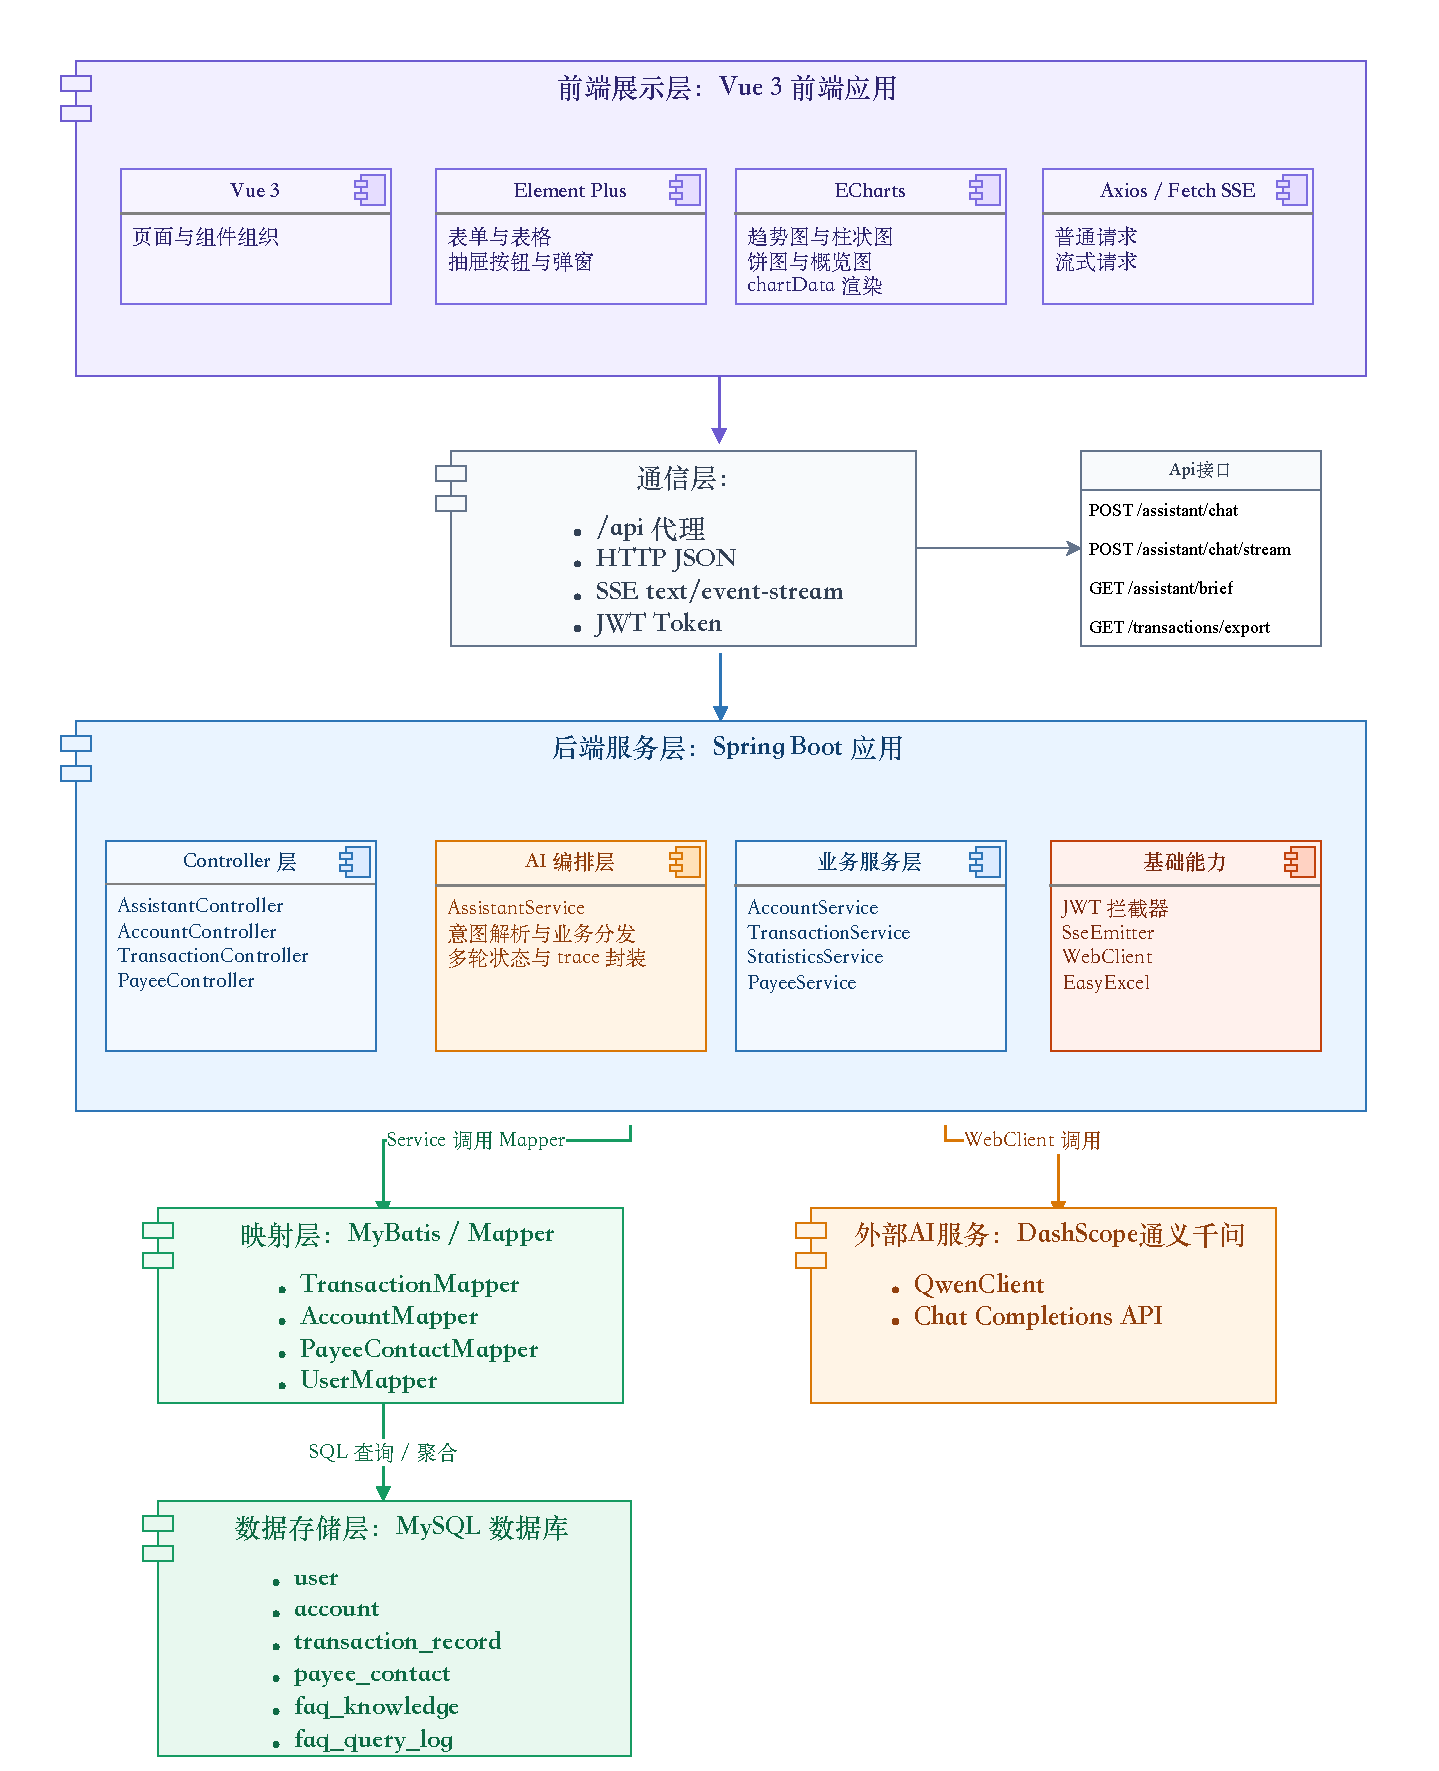
\includegraphics[width=0.92\linewidth]{image/fig-tech-stack.pdf}
    \caption{系统技术栈结构图}
\end{figure}

\chapter{系统需求分析}

\section{系统总体需求}

BankCopilot 面向银行个人用户，目标是通过智能客服机器人降低用户完成常见银行业务的操作复杂度。用户不需要记忆具体菜单和筛选条件，而是可以使用自然语言表达需求。系统应能够识别用户意图，将其映射到后端业务服务，并以文本、图表或导出文件等形式返回结果。

从用户角度看，系统需要支持账户余额查询、交易流水查询、收支统计分析、周报/月报查看和转账确认等能力。从系统角度看，AI 助手需要具备意图识别、槽位抽取、时间解析、多轮状态管理、业务服务调用、结果格式化和前端可视化展示等能力。

总体需求还体现在系统边界的划分上。AI 助手需要为用户提供更自然的入口，但不能替代后端业务规则。用户输入越口语化，系统越需要在后端建立明确的转换规则和校验逻辑。例如，用户可以说“这个月花了多少”，但后端必须把它转换为确定的起止时间、交易方向和统计指标；用户可以说“给弟弟转 300”，但后端必须识别收款人、校验金额、检查余额并等待确认。只有把自然语言表达和确定性业务规则结合起来，系统才能在银行场景中具备可用性。

此外，为满足本科毕业设计展示和答辩评阅的需要，在查看系统时，不仅需要看到 AI 回复文本，还需要看到它调用了什么业务能力、依据了哪些数据、是否存在安全确认环节。因此，本系统在需求层面就需要考虑处理过程展示、统计图表展示和快捷操作按钮。它们不是额外装饰，而是证明系统具有真实业务链路的重要交互证据。

\section{AI 核心功能需求}

\begin{table}[H]
    \centering
    \caption{AI 核心功能需求表}
    \label{tab:ai-requirements}
    \begin{tabular}{|p{0.12\linewidth}|p{0.2\linewidth}|p{0.58\linewidth}|}
        \hline
        功能编号 & 功能名称 & 需求描述 \\
        \hline
        F1 & AI 查余额 & 用户通过自然语言查询账户余额和账户基本信息，系统返回户名、账号、账户类型、状态和余额。 \\
        \hline
        F2 & AI 查流水 & 用户通过自然语言查询交易记录，系统支持收入/支出筛选、时间范围和查询条数解析。 \\
        \hline
        F3 & AI 账单统计与分析 & 用户查询总金额、笔数、最大交易或趋势时，系统基于数据库统计结果生成文本分析和图表数据。 \\
        \hline
        F4 & AI 周报/月报 & 用户打开 AI 面板时，系统展示本周或本月收入、支出、净流入、趋势、对比和异常提醒。 \\
        \hline
        F5 & AI 智能转账 & 用户通过自然语言发起转账，系统解析收款人、金额和备注，校验后等待用户确认再执行。 \\
        \hline
        F6 & AI 语音输入 & 用户点击语音输入按钮后，系统识别中文语音并回填到聊天输入框，后续按普通文本请求继续处理。 \\
        \hline
        F7 & FAQ 知识库问答 & 用户咨询银行卡挂失、转账到账时间、密码找回、验证码、贷款材料等常见问题时，系统从数据库知识库中检索并返回标准答案。 \\
        \hline
        F8 & AI 情绪安抚与人工客服引导 & 当用户表达投诉、焦虑、愤怒或担心等异常情绪时，系统先进行简短安抚，并提示拨打虚拟客服电话联系人工客服。 \\
        \hline
    \end{tabular}
\end{table}

除上述功能外，系统还需要提供 AI 基础设施能力，包括自然语言意图识别、时间范围纠偏、SSE 流式响应、AI 处理过程展示、统计口径解释和 Excel 导出链接生成等。这些能力本身不是用户直接提出的业务目标，但对提升交互体验和系统可解释性具有重要作用。

\section{非功能性需求}

安全性方面，系统必须保证用户只能查询自己的账户和流水数据，资金流动操作必须经过校验和二次确认。AI 转账不能在用户首次输入后直接扣款，必须先生成确认信息，待用户回复“确认”后才能执行。对方账号在聊天回复中应进行脱敏展示。

准确性方面，系统中的账户余额、流水记录和统计金额必须来自数据库查询结果，不得由大模型直接编造。模型输出的统计总结应受到后端事实约束，若模型返回不合适内容，系统需要使用规则化后备总结。

可用性方面，系统需要支持口语化输入，如“查一下我的余额”“看最近 7 天支出趋势”“给弟弟转 300 元”等。对于缺失关键信息的请求，系统应通过多轮对话引导用户补全，而不是直接报错。

交互性方面，AI 助手应尽量减少用户等待感和理解成本。系统通过流式响应展示处理过程，通过图表展示统计结果，通过快捷按钮完成转账确认或简报追问，从而提高交互效率。

可维护性方面，系统应保持前后端职责清晰。前端负责交互展示和用户输入收集，后端负责业务判断和数据访问，大模型调用被封装在独立客户端中。这样做的好处是，当后续需要更换模型、调整提示词或增加统计指标时，可以优先修改 QwenClient、AssistantService 或 StatisticsService，而不需要大范围改动前端页面和数据库结构，清晰的模块划分有利于该系统设计的后续维护与迭代升级。

\begin{figure}[H]
    \centering
    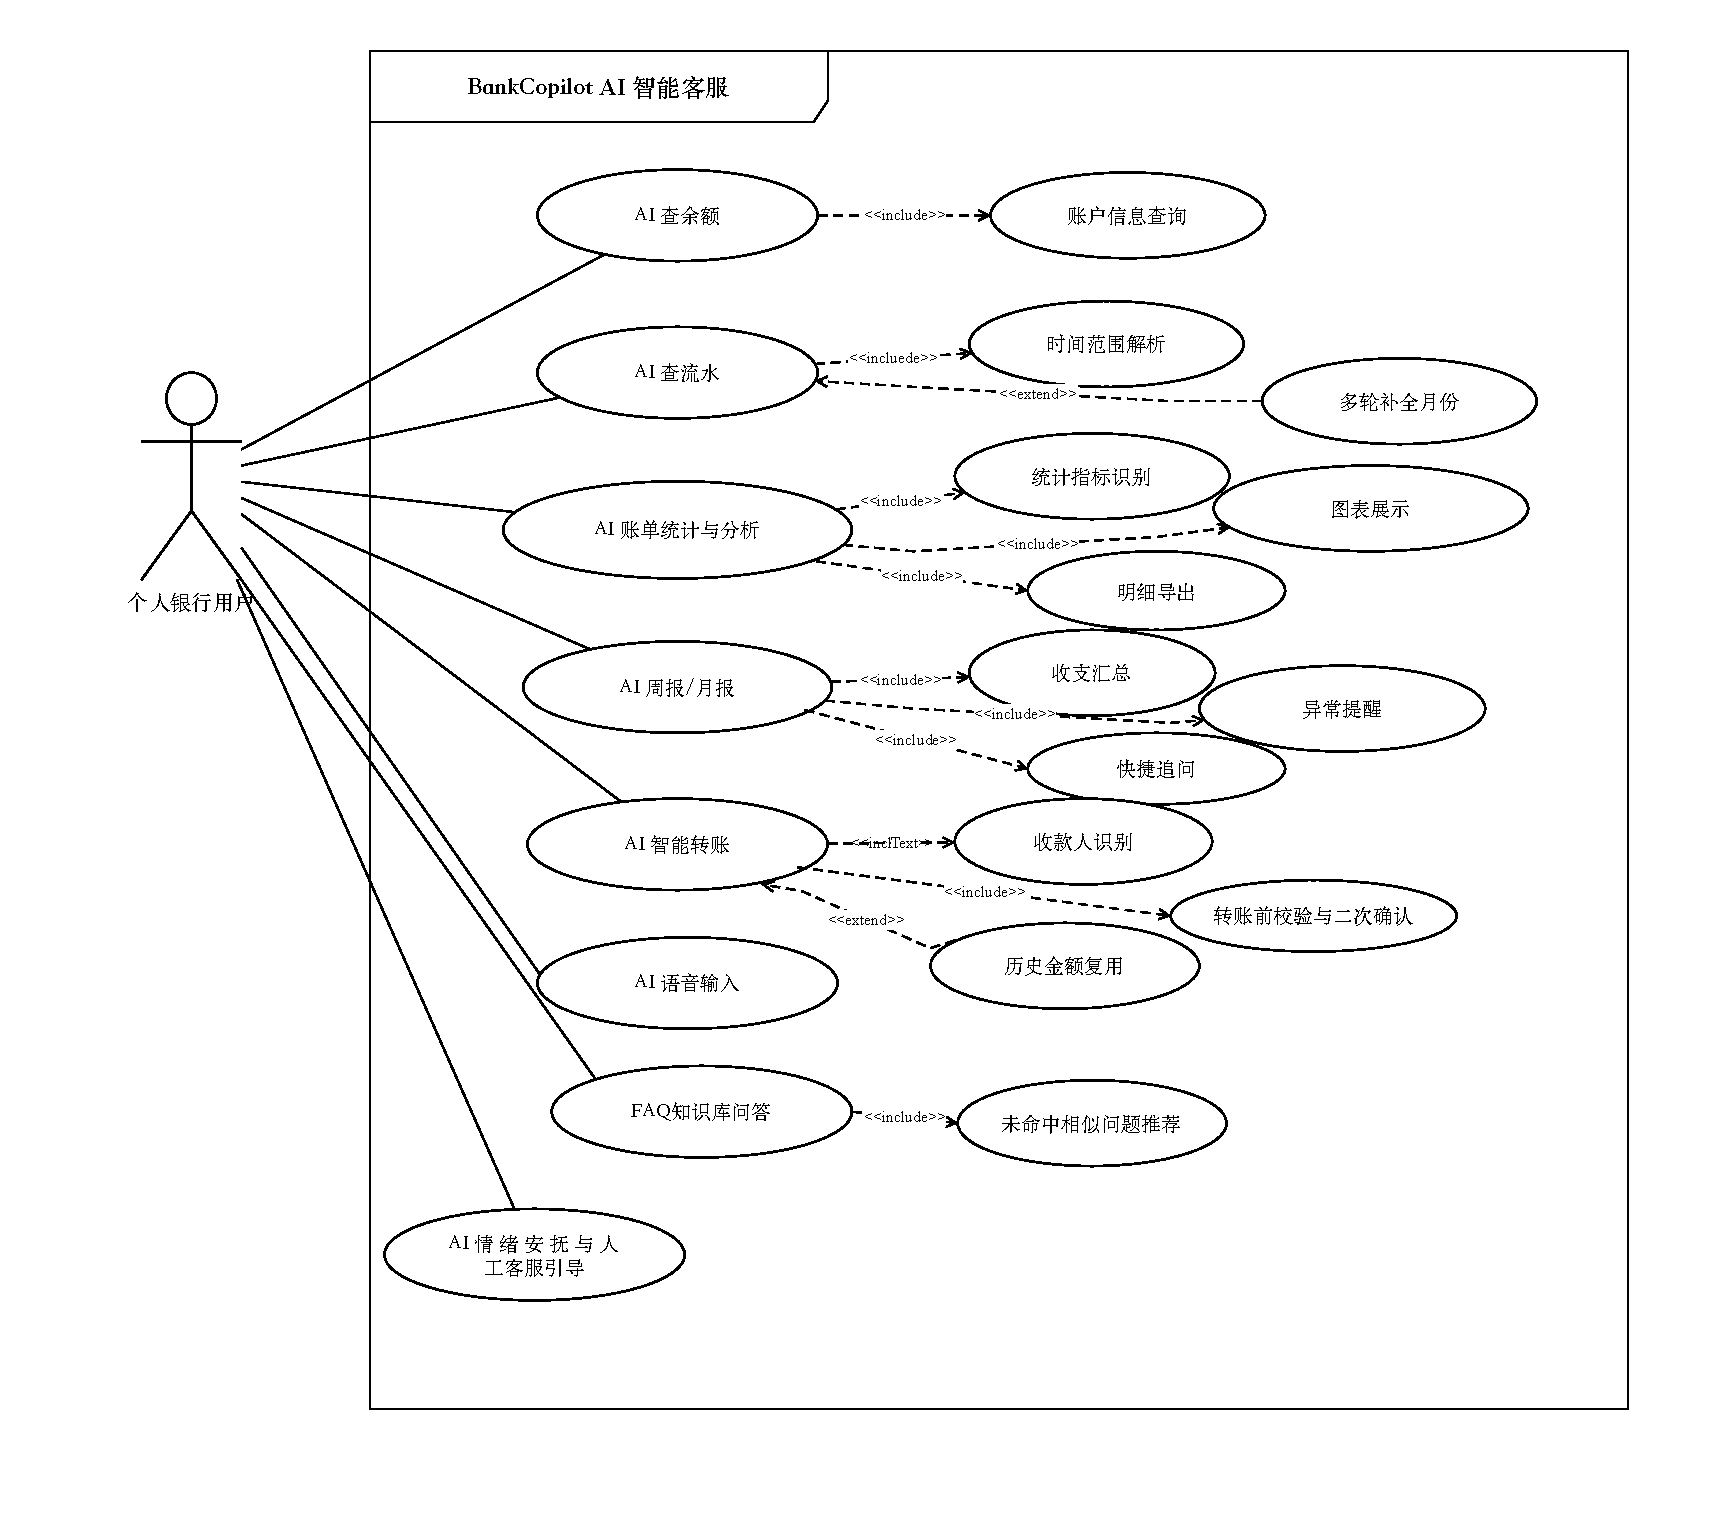
\includegraphics[width=0.92\linewidth]{image/fig-ai-usecase.pdf}
    \caption{AI 智能客服用例图}
\end{figure}

\chapter{系统总体设计}

\section{系统架构设计}

系统采用前后端分离架构。前端由 Vue 3 应用负责页面展示和用户交互，后端由 Spring Boot 应用负责业务处理和数据访问，MySQL 负责数据持久化，DashScope 通义千问负责自然语言意图解析和分析性回复生成。前端通过 /api 代理访问后端接口，后端通过 WebClient 访问大模型服务。系统总体架构如图\ref{fig:system-architecture} 所示。

\begin{figure}[H]
    \centering
    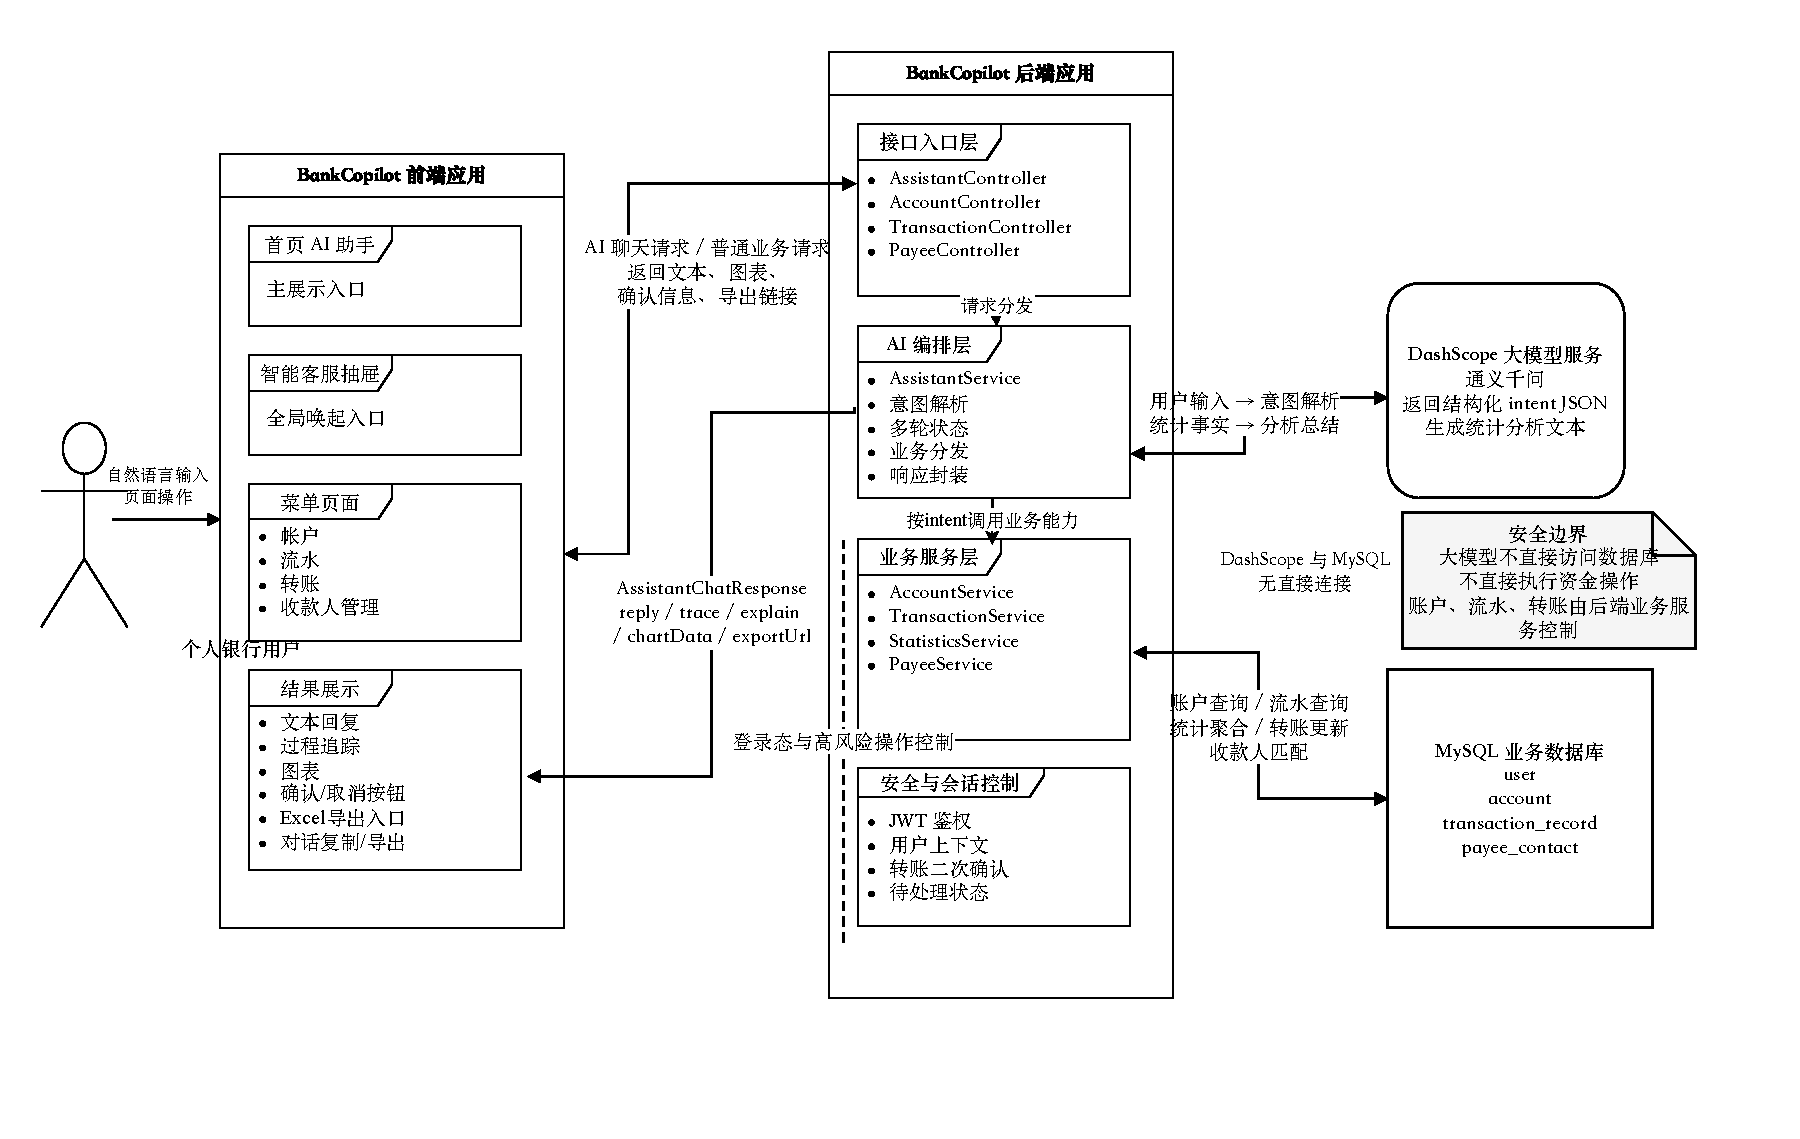
\includegraphics[width=0.86\linewidth]{image/fig-system-architecture.pdf}
    \caption{系统总体架构图}
    \label{fig:system-architecture}
\end{figure}

在该架构中，AI 助手并不是独立于业务系统之外的聊天模块，而是业务系统的一层自然语言交互入口。用户通过前端智能助手输入自然语言请求后，请求先进入后端接口层，再进入 AI 编排层；系统通过 DashScope 完成业务意图解析，并根据 intent 字段分发到账户、流水、统计或收款人服务，查询 MySQL 数据库后将结果封装返回前端。
需要强调的是，大模型无法直接访问数据库，也不执行资金操作，账户、流水和转账均由后端业务服务控制。
因此，系统架构层面的核心设计不是“在页面上增加一个聊天窗口”，而是把 AI 助手嵌入传统业务链路：前端负责收集自然语言输入和展示处理过程，AI 编排层负责把输入转换为可执行任务，业务服务层负责提供事实数据和执行结果。通过这种分层，系统既保留传统银行业务系统的确定性，又为高频查询和咨询提供更短的自然语言入口。

\section{AI 模块设计}

AI 模块由接口层、编排层、模型调用层、业务服务层、知识库服务层和前端展示层组成。接口层对应 AssistantController，提供 /assistant/chat、/assistant/chat/stream 和 /assistant/brief 三类接口。编排层对应 AssistantService，负责处理待确认状态、调用 parseIntentByQwen、根据 intent 字段分发业务流程、封装 trace 和 explain。模型调用层由 QwenClient 实现，统一封装通义千问请求。业务服务层包括 AccountService、TransactionService、StatisticsService 和 PayeeService。知识库服务层由 FaqKnowledgeService 和 FaqKnowledgeMapper 实现，负责常见问题检索和查询日志记录。前端展示层由 AssistantPanel 负责，同时包含语音输入按钮和语音识别状态展示。

这种模块划分的核心思想是“模型不直接接触数据库，业务不依赖模型自由发挥”。如图\ref{fig:ai-request-architecture}，AssistantService 处于 AI 模块的中心位置，它既要理解模型返回的意图字段，又要根据业务规则决定是否继续执行。对于普通查询，服务层可以直接调用账户或流水服务；对于缺少月份的流水查询，服务层会保存待补全状态并追问用户；对于转账请求，服务层会生成待确认对象并等待用户下一轮确认。不同业务路径虽然都从聊天输入开始，但后端处理策略并不相同。

AI 模块还承担结果适配工作。业务服务返回的通常是对象、列表或聚合数据，而用户更希望看到简明文本、图表和下一步操作入口。因此 AssistantService 会把业务结果转换为 AssistantChatResponse，前端再根据 chartType、chartData、trace、explain 和 exportUrl 等字段决定如何展示。该设计使回复内容和展示形式解耦，可以在不破坏原有接口的基础上扩展，增加新的图表类型或统计指标。
由此可见，AI 模块承担的是“业务入口、服务编排和表达适配”三类职责，而不是替代账户、流水、统计和转账服务本身。这种职责边界是本文系统设计创新的基础，也是后续安全控制、可解释展示和测试验证能够成立的前提。

\begin{table}[H]
    \centering
    \caption{AI 模块主要职责}
    \label{tab:ai-module-source}
    \begin{tabular}{|p{0.18\linewidth}|p{0.27\linewidth}|p{0.45\linewidth}|}
        \hline
        模块 & 源码位置 & 主要职责 \\
        \hline
        AI 接口入口 & AssistantController.java & 接收聊天请求、流式聊天请求和简报请求。 \\
        \hline
        AI 编排服务 & AssistantService.java & 意图解析、业务分发、多轮状态、FAQ 后备处理、统计总结。 \\
        \hline
        模型调用 & QwenClient.java & 调用通义千问 Chat Completions 接口。 \\
        \hline
        知识库检索 & FaqKnowledgeService.java & 检索 FAQ 知识库，返回直接命中、相似推荐或未命中结果。 \\
        \hline
        时间处理 & Time.java & 自然语言时间纠偏和时间范围填充。 \\
        \hline
        前端面板 & AssistantPanel.vue & 聊天、语音输入、简报、图表、过程追踪和确认按钮展示。 \\
        \hline
    \end{tabular}
\end{table}

\begin{figure}[H]
    \centering
    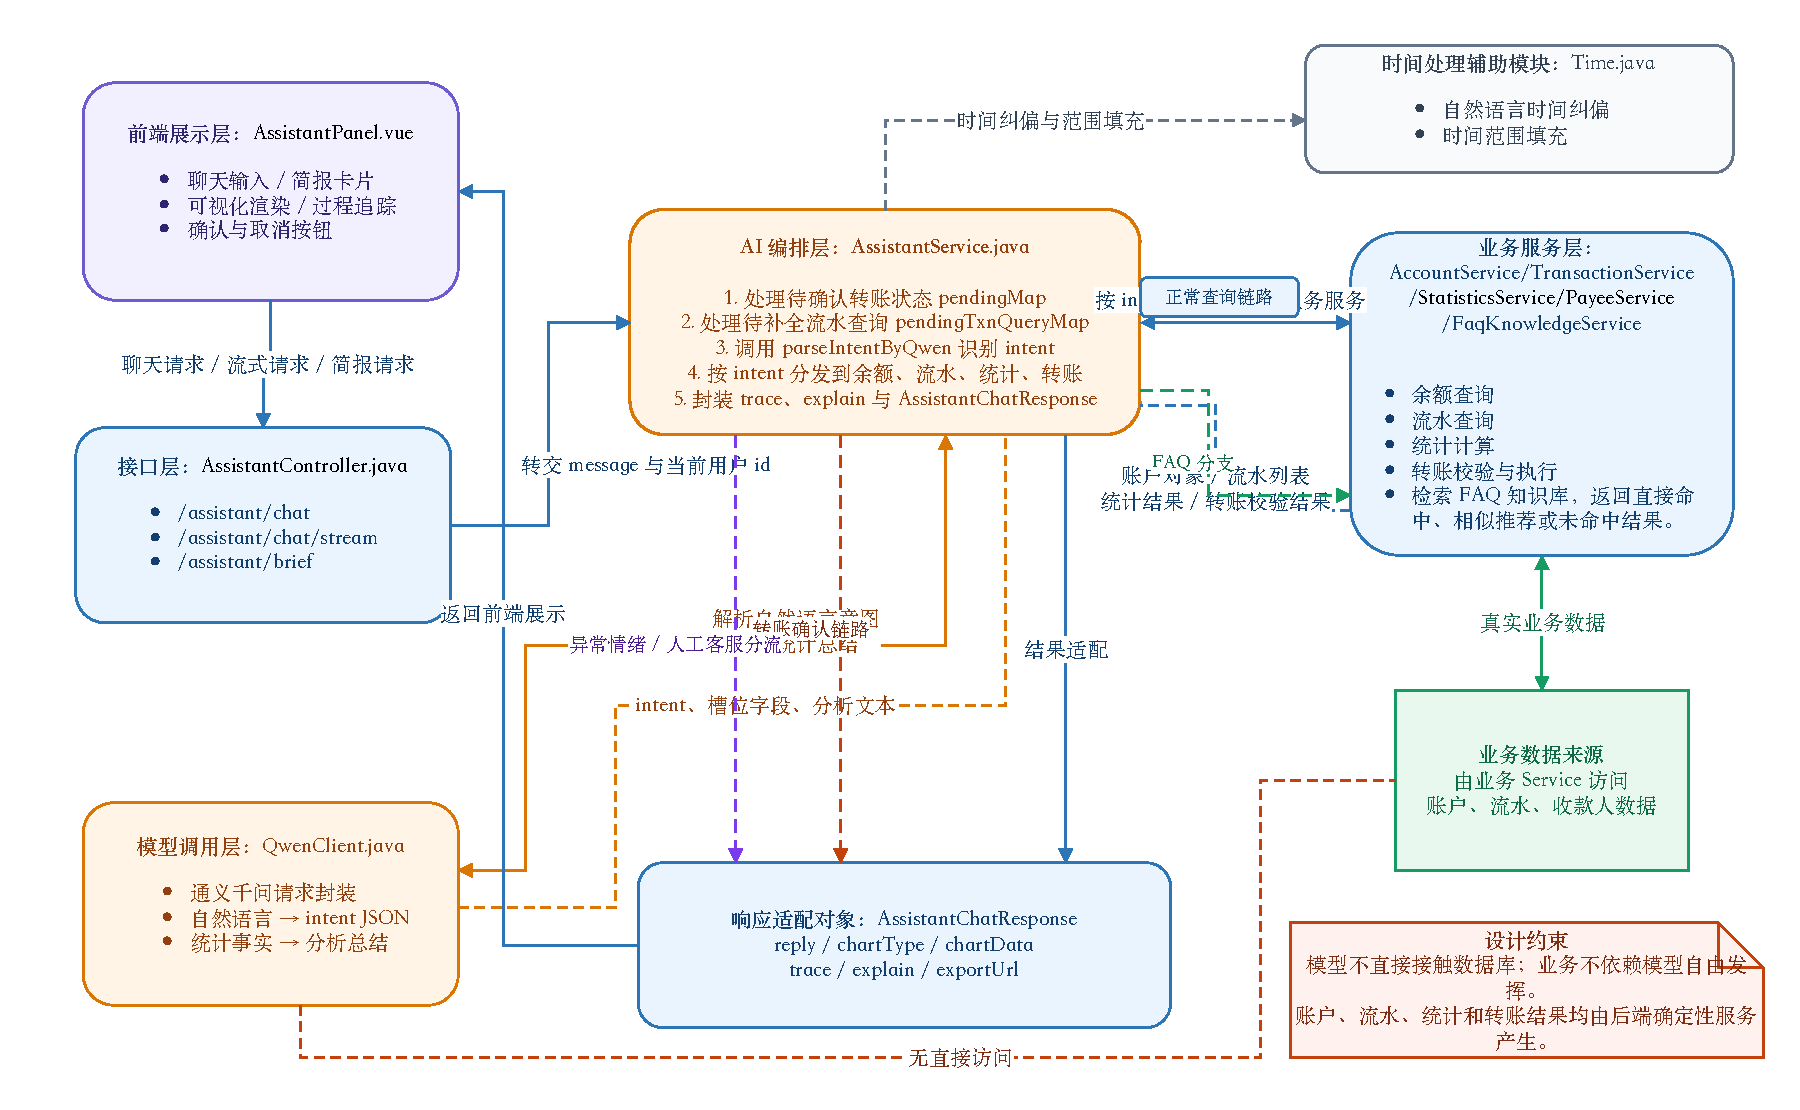
\includegraphics[width=0.92\linewidth]{image/fig-ai-request-architecture.pdf}
    \caption{AI 请求处理架构图}
    \label{fig:ai-request-architecture}
\end{figure}

\section{数据库设计}

系统 AI 功能依赖的核心数据表包括 account、transaction\_record、payee\_contact、user、faq\_knowledge 和 faq\_query\_log。AI 查余额主要读取 account 表和 user 表；AI 查流水和账单统计主要读取 transaction\_record 表；AI 智能转账需要读取 account 表、payee\_contact 表，并在执行后写入 transaction\_record 表；FAQ 知识库问答读取 faq\_knowledge 表，并把检索结果写入 faq\_query\_log 表，便于后续测试统计。为补充测试数据来源，系统还设计 assistant\_test\_log 表记录 AI 助手请求处理耗时、结果状态、意图、工具调用和回复长度等指标。

\begin{table}[H]
    \centering
    \caption{AI 功能相关数据表说明}
    \label{tab:ai-database}
    \begin{tabular}{|p{0.25\linewidth}|p{0.65\linewidth}|}
        \hline
        数据表 & 用途 \\
        \hline
        user & 保存用户基本信息，为账户户名和登录用户上下文提供支持。 \\
        \hline
        account & 保存银行账号、账户类型、余额和状态，是查余额和转账的基础表。 \\
        \hline
        transaction\_record & 保存收入、支出、金额、对方账号、备注和交易时间，是流水查询和统计分析的数据来源。 \\
        \hline
        payee\_contact & 保存用户收款人、银行卡号和昵称，用于 AI 按昵称转账。 \\
        \hline
        faq\_knowledge & 保存 FAQ 分类、标准问题、相似问法、关键词、标准答案和启用状态，用于常见问题知识库检索。 \\
        \hline
        faq\_query\_log & 保存用户原始问题、命中 FAQ、匹配得分和结果类型，用于统计知识库命中率和未命中问题。 \\
        \hline
        assistant\_test\_log & 保存 AI 助手测试和运行指标，包括请求来源、场景、意图、调用工具、处理状态、耗时和结果状态，用于补充第七章测试数据来源。 \\
        \hline
    \end{tabular}
\end{table}

\begin{figure}[H]
    \centering
    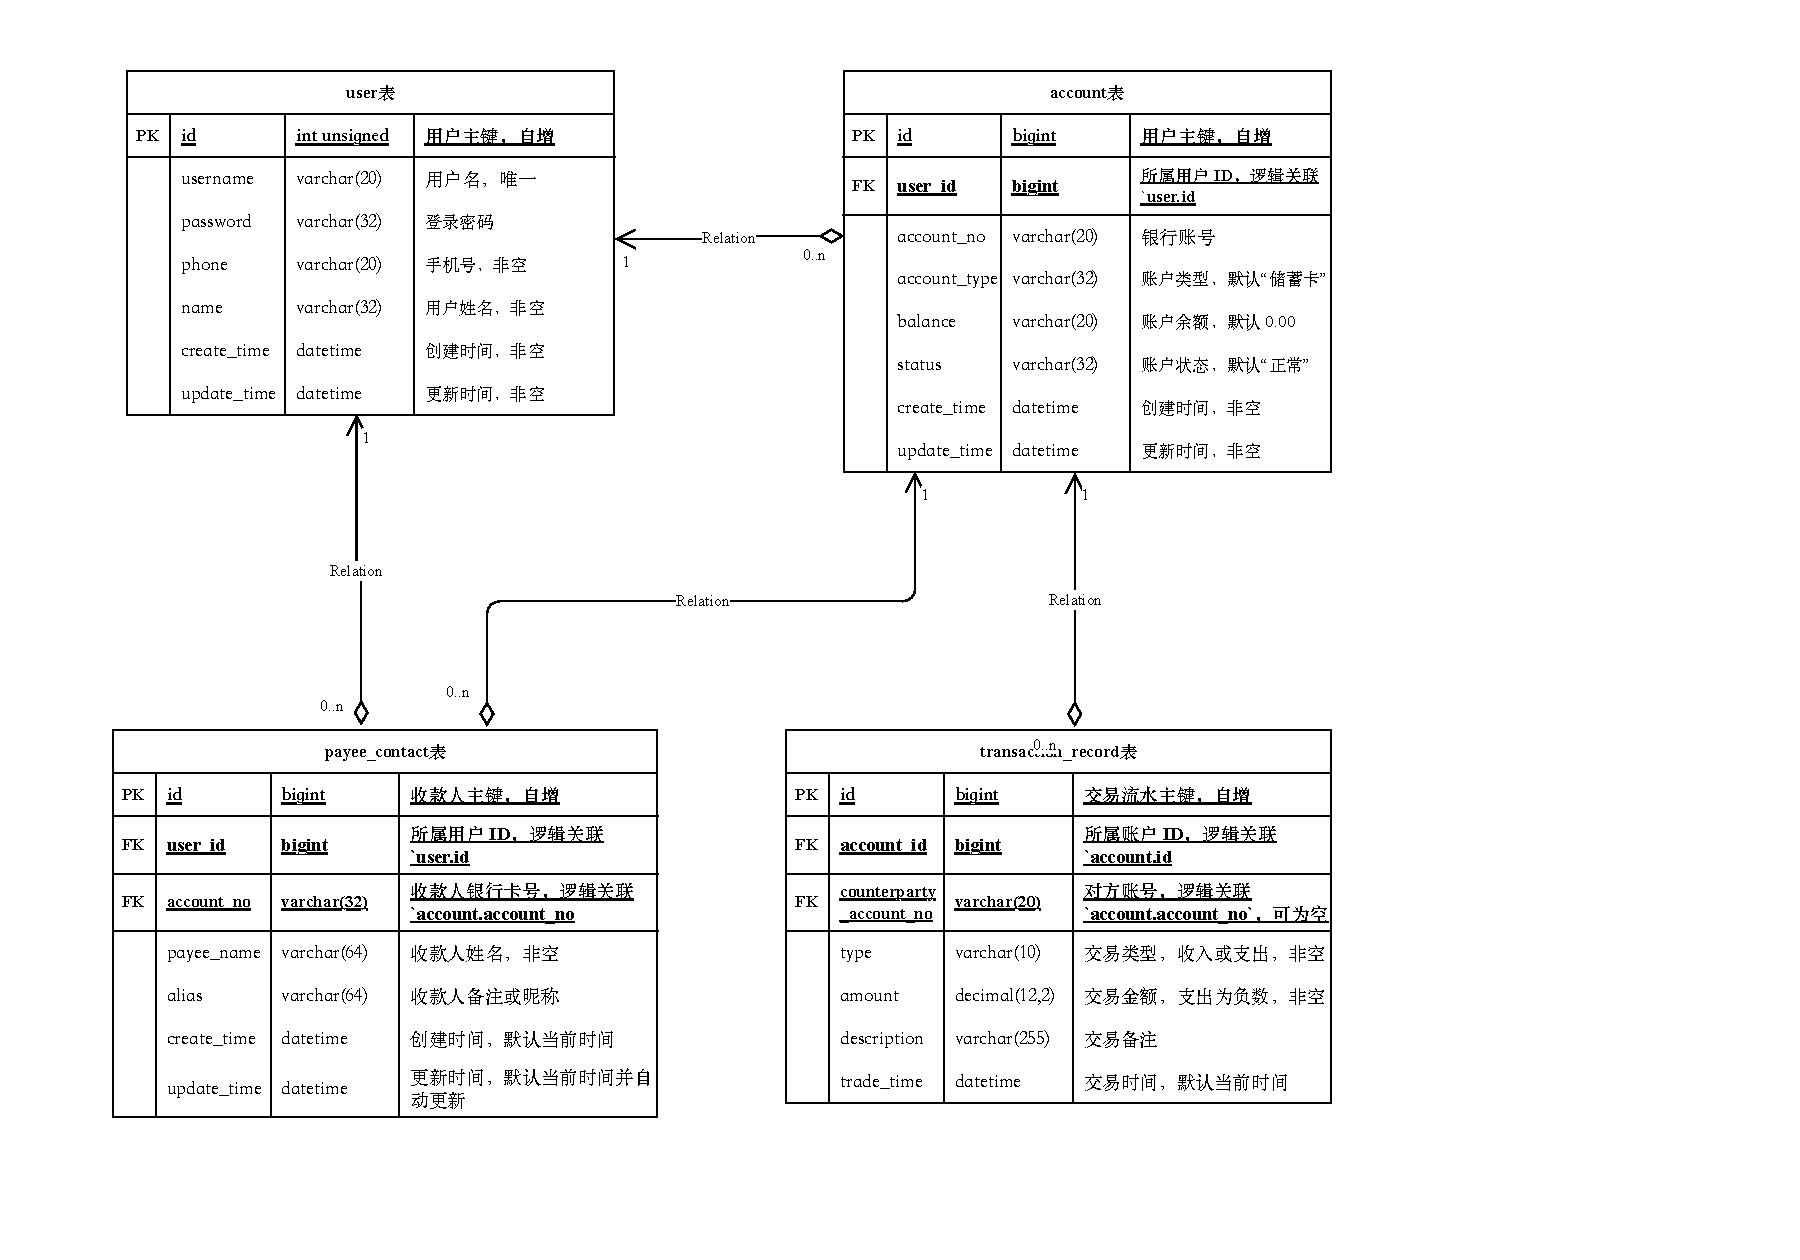
\includegraphics[width=0.92\linewidth]{image/fig-database-er.pdf}
    \caption{数据库 ER 图}
\end{figure}

\section{接口与交互设计}

AI 相关接口主要包括普通聊天接口、流式聊天接口，简报接口以及Excel导出接口。普通聊天接口用于非流式请求或流式失败后的降级处理；流式聊天接口用于提升用户等待体验；简报接口用于获取周报或月报数据；导出接口用于导出明细数据Excel。

\begin{table}[H]
    \centering
    \caption{AI 相关接口设计表}
    \label{tab:ai-api}
    \begin{tabular}{|p{0.3\linewidth}|p{0.14\linewidth}|p{0.46\linewidth}|}
        \hline
        接口 & 方法 & 功能 \\
        \hline
        /assistant/chat & POST & 普通 AI 聊天请求，返回完整 AssistantChatResponse。 \\
        \hline
        /assistant/chat/stream & POST & SSE 流式 AI 聊天请求，返回 trace、message、done 等事件。 \\
        \hline
        /assistant/brief & GET & 获取 AI 周报或月报简报。 \\
        \hline
        /transactions/export & GET & 根据统计口径导出交易流水 Excel。 \\
        \hline
    \end{tabular}
\end{table}

前端交互设计上，AI 面板既可作为首页主体展示，也可通过右上角智能客服抽屉打开。面板顶部展示周报/月报卡片，中间展示聊天记录和图表，底部提供文本输入框、演示脚本按钮、语音输入按钮和发送按钮。当 AI 回复等待转账确认时，前端显示确认和取消快捷按钮。

接口设计遵循前后端分离项目的基本原则。普通聊天接口适合一次性返回结果，便于调试和后备处理；流式聊天接口适合实际交互，可以让前端先显示处理步骤，再显示最终回复；简报接口面向页面初始化场景，用户打开 AI 面板即可看到近期账户概览。语音识别不新增后端接口，识别结果直接进入原有聊天输入框。不同接口服务于不同交互时机，避免把所有逻辑都压在单一接口中，也便于后续测试和维护。

\chapter{AI 智能客服核心功能设计与实现}

本章对应第一章和第二章提出的主要创新点与优化措施，重点说明其在系统中的具体实现方式。其中，6.1 说明 AI 请求处理总体流程和多轮状态优先机制，对应自然语言业务入口、对话管理和过程展示；6.2 说明语音转文字输入，对应交互入口扩展；6.3 和 6.4 分别说明异常情绪安抚、人工客服引导和 FAQ 知识库问答，对应客服分流和知识库建设；6.5 至 6.8 说明余额、流水、统计和周报/月报功能，对应大模型与后端确定性服务分工、统计解释和主动简报；6.9 说明智能转账二次确认、历史金额复用和取消回退，对应风险操作控制。通过这些实现，本文将前文提出的优化措施落实为可演示、可测试的系统功能。

\section{AI 请求处理总体流程}

AssistantService 的 chat 方法是 AI 请求处理的核心入口。该方法首先校验用户输入是否为空，然后优先处理待确认转账和待补全流水查询。如果当前用户存在未完成的多轮状态，则根据用户输入继续处理该状态；若不存在，则先对明显负面情绪或投诉表达进行规则检测，再调用 parseIntentByQwen 解析新请求的意图。解析完成后，系统根据 intent 字段分发到 handleTransfer、handleTransactions、handleBalance、handleStatistics 或 handleFaqOrFallback。其中 handleFaqOrFallback 会先检索 FAQ 知识库，无法命中时再进入原有后备回复。

\begin{figure}[H]
    \centering
    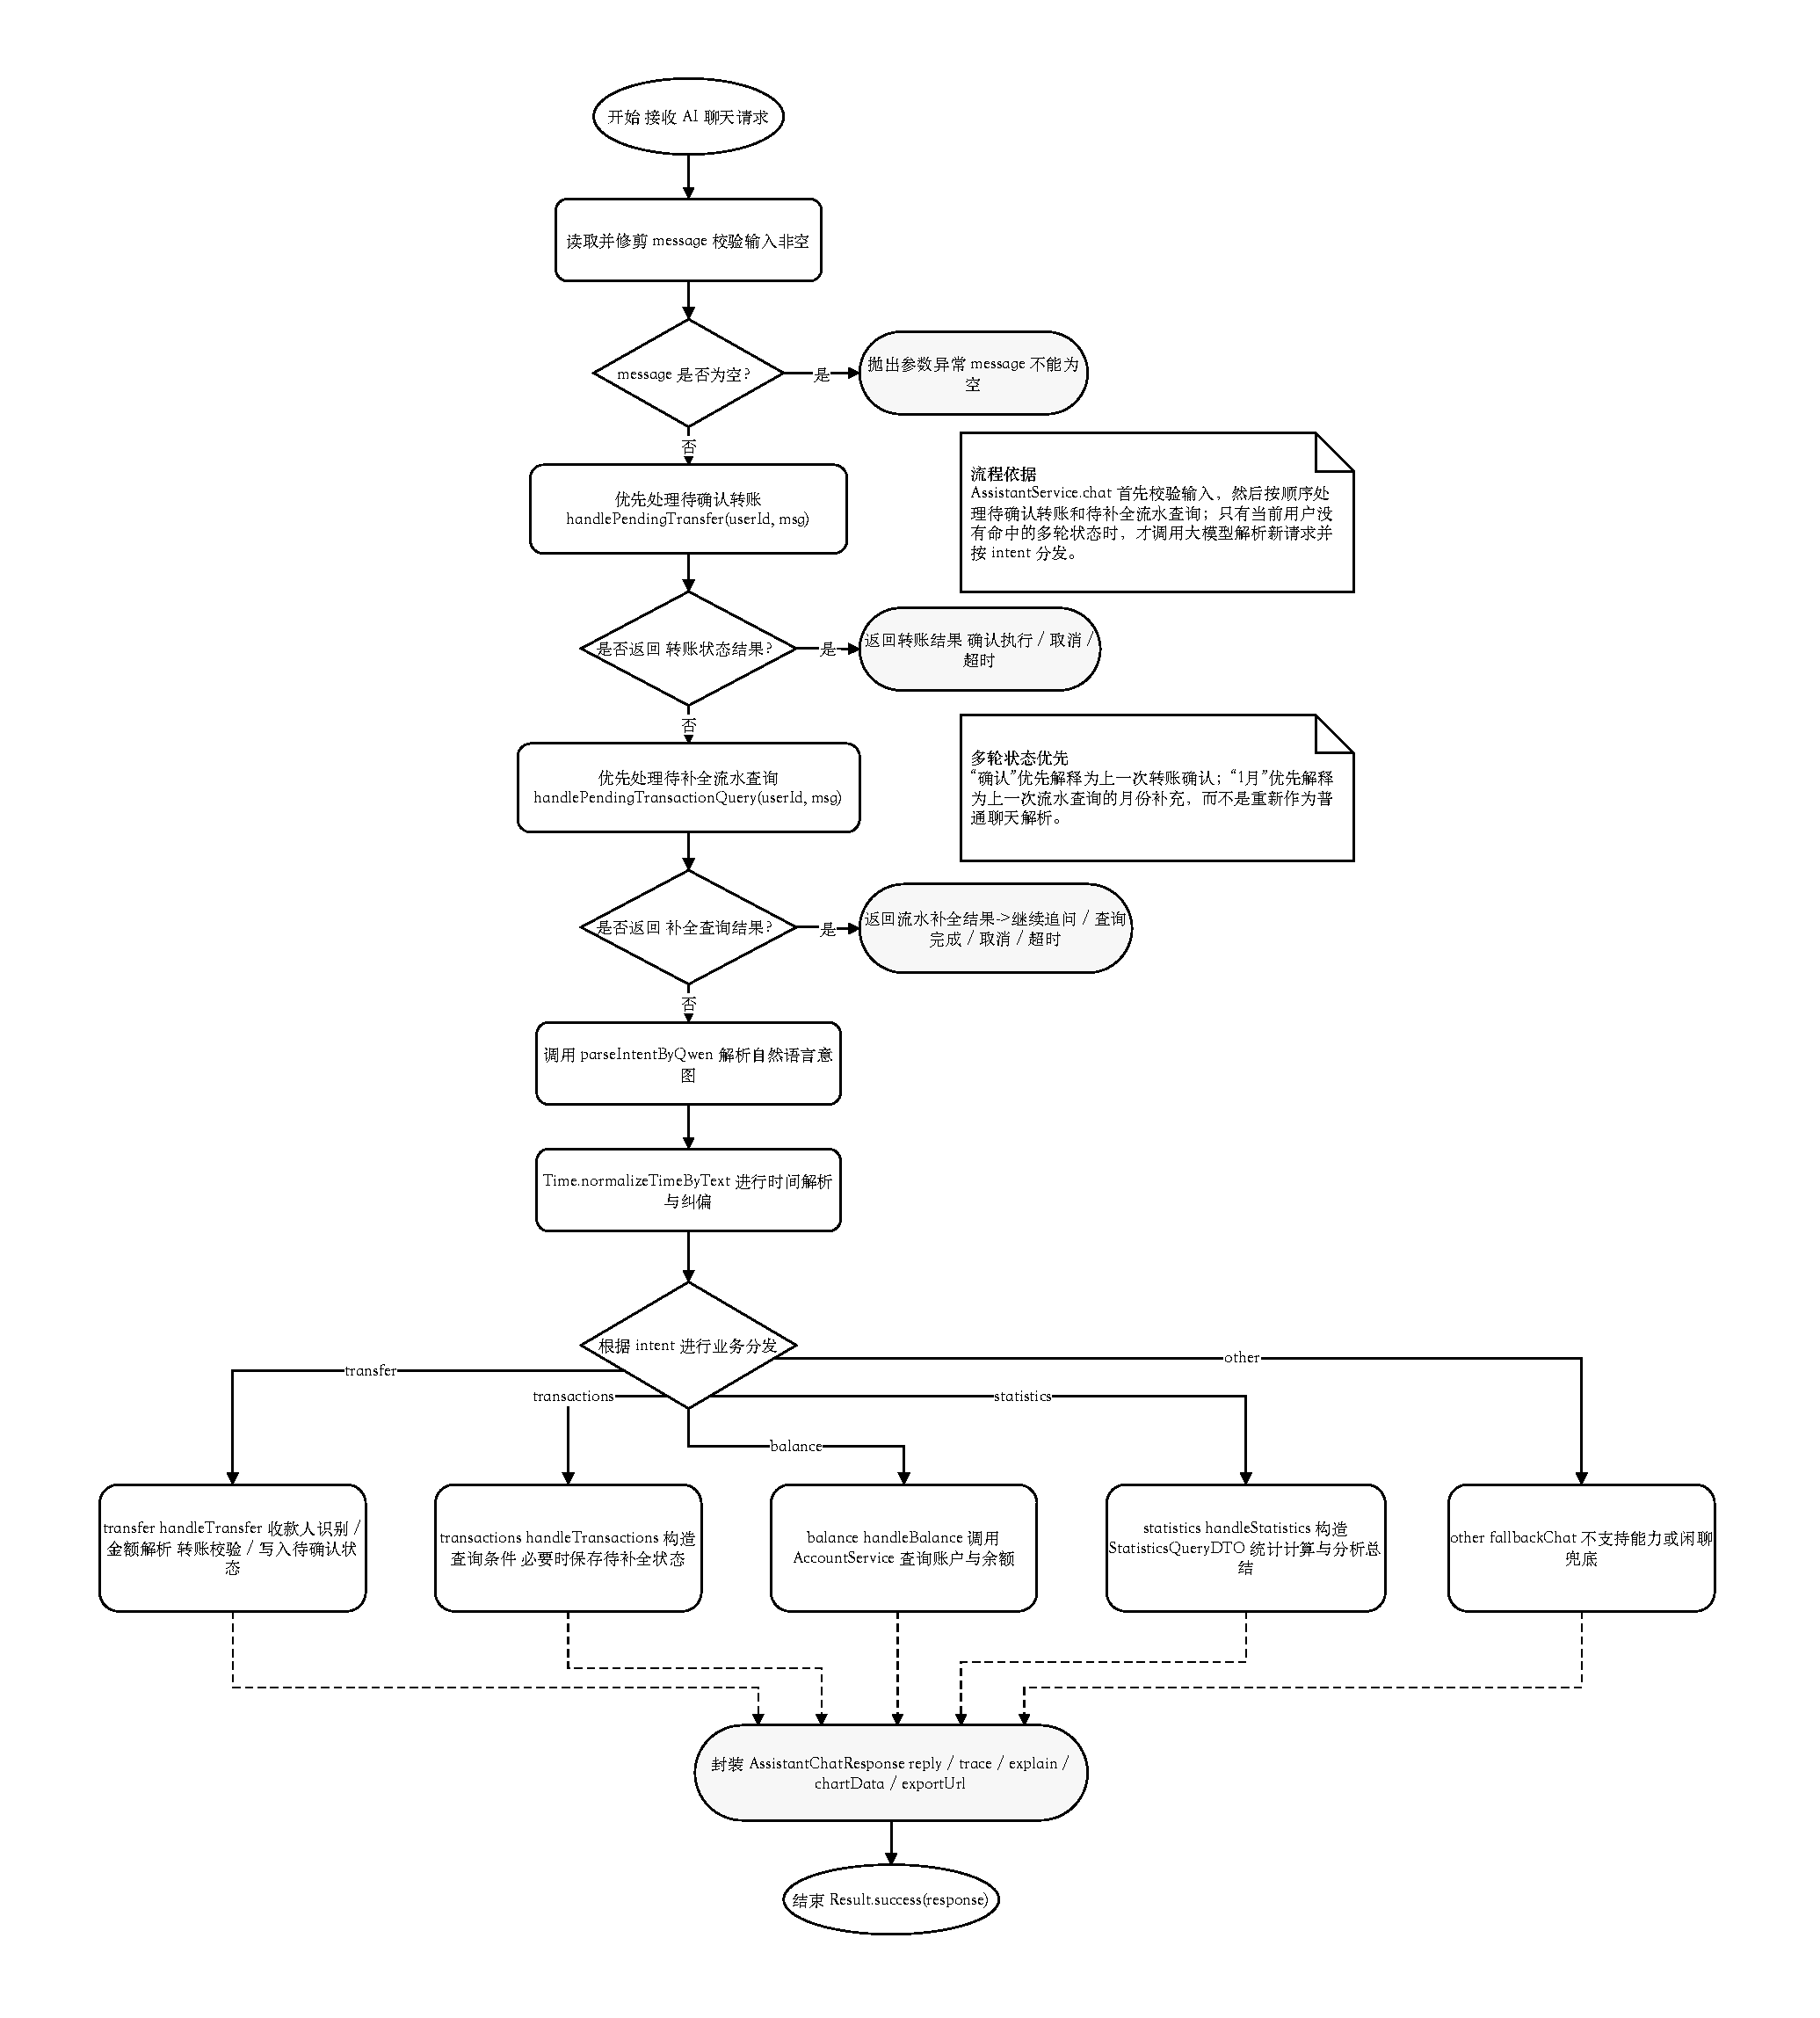
\includegraphics[width=1.22\linewidth]{image/fig-ai-chat-flow.pdf}
    \caption{AI 聊天请求总体流程图}
\end{figure}

该流程体现了“多轮状态优先，新请求解析其次”的设计思路。例如用户发起转账后，系统等待“确认”或“取消”，此时下一条用户输入应优先作为转账确认处理，而不是重新解析为普通聊天请求。类似地，当用户查询“17 号收入记录”但缺少月份时，系统会等待用户补充月份，下一条“1 月”应被视为补全条件。

这种处理顺序符合聊天式业务系统的实现规律。单轮问答只需要根据当前输入返回结果，而银行客服机器人需要处理用户前后两轮输入之间的关系。如果不维护状态，系统就无法判断“确认”到底确认什么，也无法判断“1 月”是在补充哪个查询。

在响应结构上，系统不仅返回 reply，还返回 trace、chartData、exportUrl 和 explain 等字段。reply 面向普通用户，强调可读性；trace 面向可解释性和调试，说明识别意图、调用工具和处理步骤；chartData 面向前端图表展示；exportUrl 面向交易流水导出；explain 面向统计口径说明。通过这些结构化字段，前端可以把一次 AI 回复拆分为文本、图表、过程和操作入口，使系统更像一个完整的智能业务助手，而不是简单聊天窗口。

\section{AI 语音输入功能实现}

语音输入功能主要在前端中实现，调用浏览器语音识别能力完成中文语音转写，系统面向中文短句输入，允许在识别过程中把临时结果及时显示到输入框中。

用户点击“语音输入”按钮后，toggleVoiceInput 方法会启动语音识别，并将 voiceListening 设置为 true。识别过程中，onresult 事件会读取 event.results 中的转写文本，并通过 mergeSpeechText 方法与原输入框内容合并，最终写入 chatInput。用户可以在识别后继续手动修改文本，也可以直接点击发送按钮。后续流程与普通文本输入完全一致，仍然由 /assistant/chat/stream 接口发送到后端，再由 AssistantService 进行意图解析、业务分发和结果封装。

该功能的设计重点是满足对语音识别交互的要求，并降低用户在移动或演示场景下的输入成本，同时，语音识别不同于输入文字的确定性，可能存在语句不通畅，字词缺失错误，语句冗长且表达意思不准确等问题，通过这些可以测试AI在面对真实交流场景下的应对和识别处理效果。由于语音识别只负责把语音转换为文本，不直接调用账户、流水、统计或转账服务，因此它不会改变原有业务安全边界。浏览器不支持语音识别、麦克风未授权或没有识别到语音内容时，前端会给出提示，用户仍可回到文本输入方式完成同一业务操作。

\section{AI 情绪安抚与人工客服引导功能实现}

情绪安抚与人工客服引导功能主要在后端 AssistantService 中实现。系统在处理转账确认和流水查询补全之后、调用大模型进行普通意图解析之前，先调用 handleEmotionSupport 方法对用户输入进行轻量级情绪检测。该检测不依赖单独训练的情感分类模型，而是通过关键词规则识别投诉、愤怒、焦虑和担心等明显表达。例如，当输入中包含“我要投诉”“投诉你们”“服务太差”“乱扣”“扣错”等词时，系统将其归为 complaint；当输入中包含“生气”“气死”“愤怒”“崩溃”等词时，系统将其归为 angry；当输入中包含“很着急”“焦虑”“担心”“害怕”等词时，系统将其归为 anxious。

当检测到异常情绪后，系统不会继续让大模型自由生成安抚内容，而是返回规则化回复。回复内容包括三部分：首先对用户当前情绪进行简短理解和安抚；其次提醒用户涉及账户和资金问题时不要重复提交操作，并说明系统仍可继续帮助查询余额、流水、统计或转账状态；最后提示用户拨打虚拟客服电话 010-1234-5678 联系人工客服。该号码用于毕业设计演示，不对应真实银行热线。

同时，由于关键词规则无法覆盖所有表达，当请求进入后备回答分支时，系统仍可生成较温和的安抚性回复。

该功能的设计边界需要明确。情绪安抚模块不参与账户余额计算、流水查询、统计聚合和转账执行，也不改变用户资金操作结果。它只是在用户出现明显负面情绪或投诉意图时提供更符合客服场景的回应，并把可能需要人工处理的问题引导到人工客服渠道。这样既回应了任务书中关于情感分析类能力和交互优化的要求，又避免把关键词检测误写为复杂情感分析模型，或误用为银行业务决策依据。

\section{FAQ 知识库问答功能实现}

FAQ 知识库问答功能用于处理不属于余额、流水、统计和转账执行的常见咨询问题。系统新增 faq\_knowledge 表保存问题分类、标准问题、相似问法、关键词、标准答案、启用状态和优先级等字段，并新增 faq\_query\_log 表记录用户原始问题、命中 FAQ、匹配得分和结果类型。这样既能满足“建立知识库存储常见问题和答案”的要求，也能为后续测试统计提供数据来源。

在处理流程上，AssistantService 对业务意图分发后，若 intent 字段为 other，则进入 handleFaqOrFallback 方法。该方法首先调用 FaqKnowledgeService.search，对用户问题和知识库中的标准问题、相似问法、关键词进行匹配。若匹配得分达到高置信度阈值，系统直接返回知识库中的标准答案；若得分处于中等区间，系统返回 2 到 3 个相似问题供用户继续选择；若知识库未命中，则再进入原有 fallbackChat 后备回复。

该设计避免让大模型自由编造银行业务规则。银行卡挂失、转账到账时间、验证码收不到、密码找回、贷款材料等问题的答案均来自 faq\_knowledge 表，而不是由模型临时生成。faq\_query\_log 表还可以统计 hit、recommend 和 no\_answer 三类结果，用于第七章分析知识库命中率、推荐命中率和未收录问题，为实验测试补充更具体的数据。

在知识库更新方面，当前系统通过数据库表维护 FAQ 内容，faq\_knowledge 表中的 status、priority 和 update\_time 字段可用于控制答案启用状态、返回优先级和更新时间。当用户问题未直接命中知识库时，系统会将原始问题、匹配结果和 result\_type 写入 faq\_query\_log 表。后续维护时，管理人员可以根据 no\_answer 和 recommend 记录补充标准问题、相似问法、关键词和标准答案，并对新增或修改内容进行审核后再启用。通过这种“查询日志反馈 + 人工维护审核 + 数据库字段控制”的方式，系统能够在原型范围内回应知识库内容及时更新的要求。

\section{AI 查余额功能实现}

AI 查余额对应 balance 意图。当用户输入“查一下我的余额”“我的账户信息”等表达时，parseIntentByQwen 会将 intent 字段解析为 balance。AssistantService 随后调用 handleBalance 方法，通过 AccountServiceImpl.getAccountInfo 查询当前登录用户的账户信息。

handleBalance 返回的内容包括户名、账号、账户类型、账户状态和余额。该功能实现虽较为直接，但它体现了系统设计中的关键原则：AI 只识别用户想查余额，余额数据本身必须来自数据库账户表，而不是来自模型生成。

余额查询功能虽然业务逻辑相对简单，但在本论文中具有基础性意义。该功能证明 AI 助手已经能够从自然语言入口进入真实后端服务，而不是只返回固定话术。同时还为后续流水查询、统计分析和转账功能提供了账户上下文基础。若余额查询无法保证数据准确，后续涉及金额分析和资金操作的功能就缺少可信前提。因此本文将其作为核心功能之一进行说明。

\begin{table}[H]
    \centering
    \caption{AI 查余额功能实现说明}
    \label{tab:balance}
    \begin{tabular}{|p{0.22\linewidth}|p{0.18\linewidth}|p{0.2\linewidth}|p{0.3\linewidth}|}
        \hline
        输入示例 & 解析意图 & 调用方法 & 返回内容 \\
        \hline
        查一下我的余额 & balance & handleBalance & 户名、账号、账户类型、状态、余额。 \\
        \hline
        我的账户信息 & balance & handleBalance & 账户基本信息和余额。 \\
        \hline
    \end{tabular}
\end{table}

\section{AI 查流水功能实现}

AI 查流水对应 transactions 意图。用户可以使用自然语言指定交易类型、时间范围和条数限制。例如“查最近 3 条支出记录”会被解析为 txnType=支出、limit=3、timeRange=latest；“查今天的流水”会被解析为 timeRange=day；“查前几天的支出记录”会经过 Time.normalizeTimeByText 纠偏为 recent\_days。

handleTransactions 方法会根据解析结果构造 TransactionQueryDTO，并调用 Time.fillTimeRange 填充 startTime 和 endTime。随后系统调用 TransactionServiceImpl.getTransactions 进行查询，底层 SQL 由 TransactionMapper.xml 中的 selectTransactions 完成。查询结果由 convertTransactionResultToChat 格式化为自然语言列表，并对对方账号进行脱敏处理。

对于缺少月份的日期查询，系统设计了多轮补全机制。当 needMonth 为 true 且存在 day 但 month 为空时，系统将当前查询保存在 pendingTxnQueryMap 中，并提示用户补充月份。用户回复“1 月”后，下一轮请求会优先进入 handlePendingTransactionQuery，而不是被当作新的普通问题重新解析。该方法会读取待补全状态、解析月份、构造 TransactionQueryDTO，并继续调用流水查询服务完成查询。

流水查询比余额查询更能体现自然语言到结构化条件的转换过程。用户表达中可能包含交易方向、相对时间、绝对日期、条数限制等多种信息，后端需要把它们映射为 TransactionQueryDTO 中的字段。由于交易流水是账单统计和历史金额复用的基础数据，查询条件的准确性直接影响后续功能结果。本文在实现中采用模型解析和规则纠偏结合的方式：模型负责理解用户表达，Time 工具负责修正时间范围，Mapper 层负责执行确定 SQL 查询。

图\ref{fig:transaction-multiturn} 以时序图形式展示了缺少月份时的两轮交互过程。第一轮中，用户提出“查17号收入记录”，系统识别为 transactions 意图并发现 month 为空，于是保存 PendingTransactionQuery 并追问月份；第二轮中，用户回复“1月”，AssistantService 优先命中 pendingTxnQueryMap，补齐日期范围后调用 TransactionService 和 TransactionMapper 完成流水查询。

\begin{figure}[H]
    \centering
    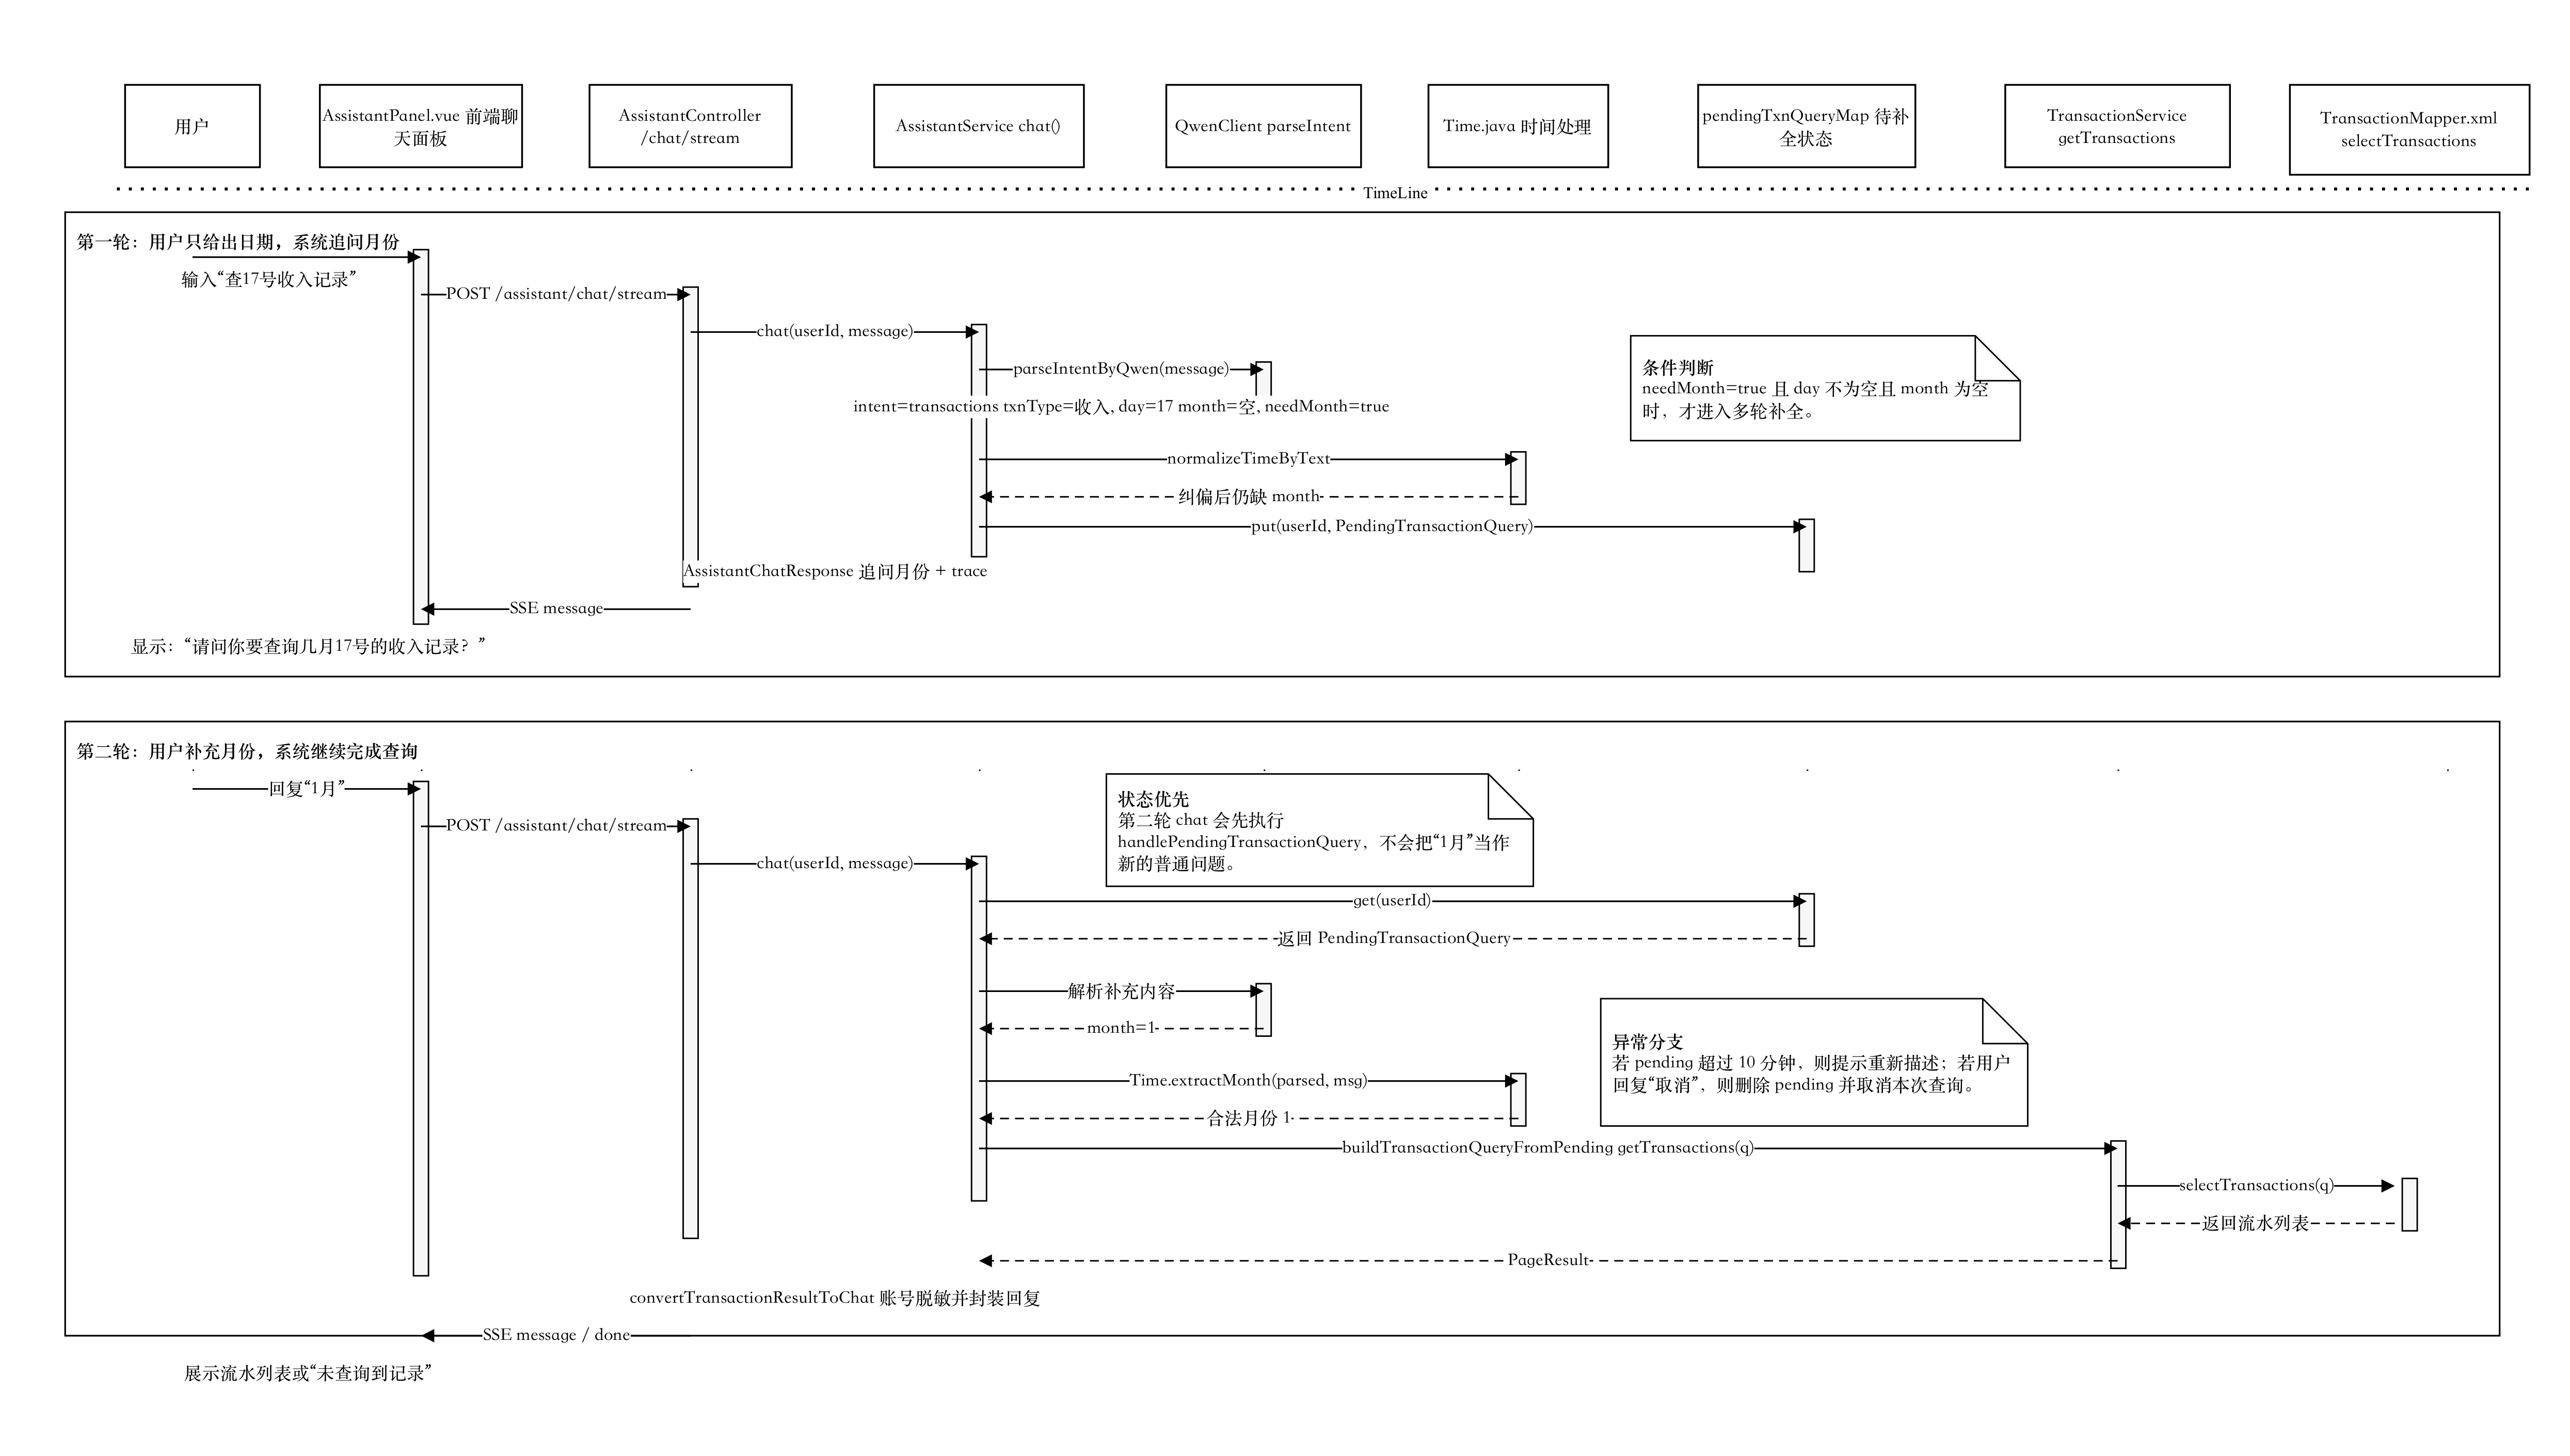
\includegraphics[width=\linewidth]{image/fig-transaction-multiturn.png}
    \caption{AI 查流水多轮补全时序图}
    \label{fig:transaction-multiturn}
\end{figure}

\begin{table}[H]
    \centering
    \caption{AI 查流水测试输入与处理方式}
    \label{tab:transaction-query}
    \begin{tabular}{|p{0.25\linewidth}|p{0.38\linewidth}|p{0.27\linewidth}|}
        \hline
        用户输入 & 关键解析字段 & 系统行为 \\
        \hline
        查最近 3 条支出记录 & txnType=支出, limit=3, timeRange=latest & 查询最近 3 条支出流水。 \\
        \hline
        查今天的流水 & timeRange=day & 查询当天全部流水。 \\
        \hline
        查前几天的支出记录 & txnType=支出, timeRange=recent\_days, rangeValue=3 & 查询近 3 天支出流水。 \\
        \hline
        查 17 号收入记录 & txnType=收入, day=17, needMonth=true & 追问月份并进入待补全状态。 \\
        \hline
    \end{tabular}
\end{table}

\section{AI 账单统计与分析功能实现}

AI 账单统计与分析对应 statistics 意图。系统支持 sum、count、max 和 trend 四类统计指标，分别用于统计总金额、流水笔数、最大一笔交易和趋势数据。用户输入“统计这个月总支出”时，系统会构造 txnType=支出、metric=sum、timeRange=month 的 StatisticsQueryDTO；用户输入“看最近 7 天支出趋势”时，系统会构造 txnType=支出、metric=trend、timeRange=recent\_days、groupBy=day 的查询对象。

\begin{table}[H]
    \centering
    \caption{统计指标与实现方法对应关系}
    \label{tab:statistics-metric}
    \begin{tabular}{|p{0.16\linewidth}|p{0.22\linewidth}|p{0.26\linewidth}|p{0.26\linewidth}|}
        \hline
        统计指标 & 含义 & 底层方法 & 前端展示 \\
        \hline
        sum & 总金额统计 & sumAmount & 数字结果或收支概览图。 \\
        \hline
        count & 笔数统计 & countByStatistics & 数字结果。 \\
        \hline
        max & 最大一笔统计 & maxTransaction & 数字结果。 \\
        \hline
        trend & 趋势统计 & statisticsTrend & 柱状图或折线图。 \\
        \hline
    \end{tabular}
\end{table}

StatisticsServiceImpl 根据 metric 调用不同 Mapper 方法。sumAmount 用于总额统计，countByStatistics 用于笔数统计，maxTransaction 用于最大一笔交易，statisticsTrend 用于趋势聚合。当用户查询整体收支概览时，系统还会通过 sumIncomeAndExpense、statisticsByCounterparty 生成收支对比和按对方账号聚合的图表数据。因此，账单统计与分析本质上是对交易流水查询能力的进一步聚合和解释：流水查询返回明细记录，统计分析则在同一数据基础上完成汇总、趋势和概览。

统计分析文本的生成采用“事实构造 + 模型总结 + 规则化后备总结”的设计。AssistantService 会将统计标题、统计类型、统计指标、时间范围、统计值、趋势明细、主要对方账号和异常信号等内容整理成 facts，然后请求通义千问生成自然语言分析总结。若模型输出为空、过于模板化或包含不支持的标签、消费类别等内容，系统会返回规则化后备总结。与上一节多轮查流水不同，统计分析功能的重点不是多个参与对象之间的消息时序，而是自然语言条件如何被转换为统计 DTO，并经过确定性 SQL 聚合、事实整理和模型表达生成完整分析结果。

图\ref{fig:statistics-analysis-flow} 展示了 AI 账单统计与分析的整体处理流程。系统先解析 statistics 意图并构造 StatisticsQueryDTO，再由 StatisticsServiceImpl 和 TransactionMapper.xml 完成总额、笔数、最大值或趋势等确定性统计。统计结果被封装为 StatisticsResultVO 后，AssistantService 进一步整理 facts 并调用大模型生成分析总结；当模型输出不符合约束时，系统使用规则化后备总结，最后将 reply、chartData、explain 和 exportUrl 等字段返回前端展示。

\begin{figure}[H]
    \centering
    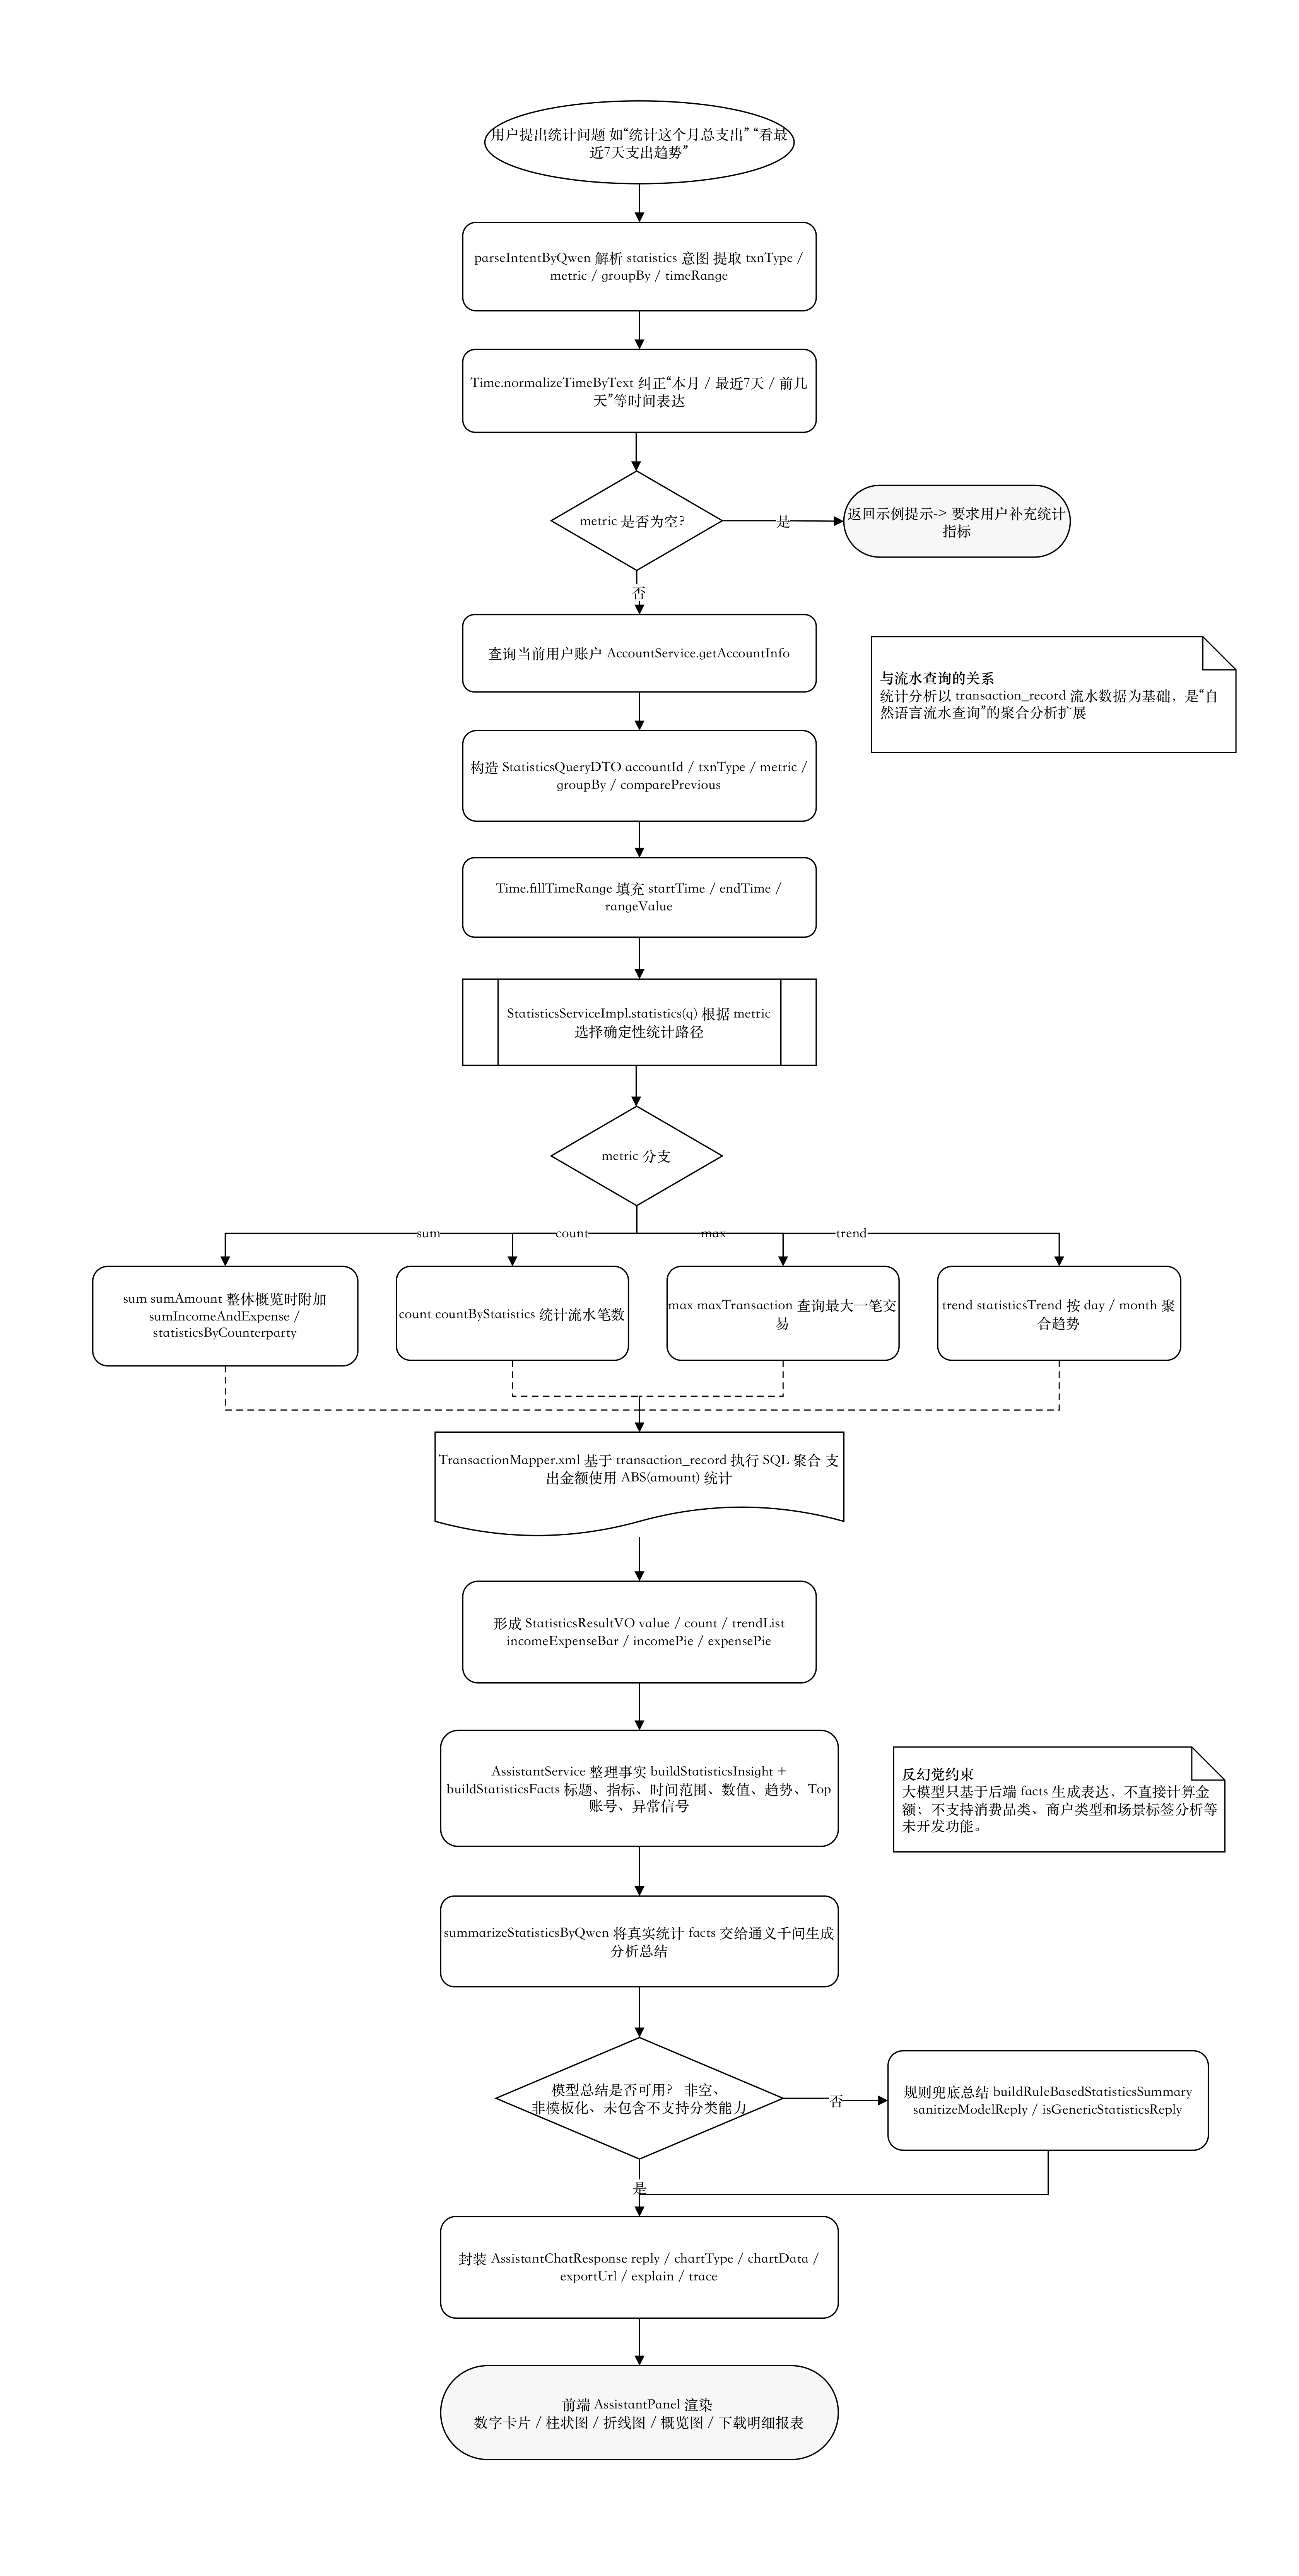
\includegraphics[width=0.88\linewidth]{image/fig-statistics-analysis-flow.png}
    \caption{AI 账单统计与分析流程图}
    \label{fig:statistics-analysis-flow}
\end{figure}

前端根据 AssistantChatResponse 中的 chartType 和 chartData 渲染图表。chartType 为 number 时显示数字卡片，为 bar 或 line 时显示趋势图，为 overview 时显示收支对比柱状图和收入、支出按对方账号聚合的饼图。系统还会生成 exportUrl，用户可以下载当前统计口径下的交易流水 Excel 文件。

\begin{figure}[H]
    \centering
    \IfFileExists{image/fig-ai-statistics-chart-ui.png}{
        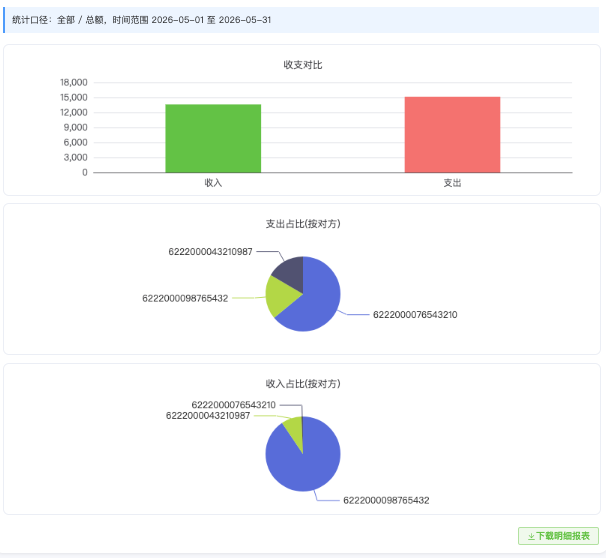
\includegraphics[width=0.92\linewidth]{image/fig-ai-statistics-chart-ui.png}
    }{
        \fbox{\parbox[c][0.34\linewidth][c]{0.86\linewidth}{\centering 待补充截图：image/fig-ai-statistics-chart-ui.png}}
    }
    \caption{AI 账单统计与图表展示界面图}
    \label{fig:ai-statistics-chart-ui}
\end{figure}

\section{AI 周报/月报功能实现}

AI 周报/月报由 /assistant/brief 接口提供，主要用于用户打开 AI 面板时自动展示财务概览。该功能不依赖用户主动提问，而是根据 period 参数生成 week 或 month 简报。

getBrief 方法会先查询当前用户账户，然后构造收入总额、支出总额和支出趋势三个统计查询。系统计算总收入、总支出和净流入，并进一步生成与上周或上月的对比数据。对于异常提醒，系统使用近 4 周平均支出和近 30 天支出金额 P90 阈值作为参考，检测当前周期支出是否明显偏高或是否存在超大单笔支出。

前端 AssistantPanel 在 mounted 阶段调用 fetchAssistantBriefApi 加载简报，并在面板顶部展示 headline、highlights、suggestions、anomalies、comparison、quickActions 和 chartData。用户可以在周报和月报之间切换，也可以点击快捷追问按钮继续向 AI 发起查询。

\begin{figure}[H]
    \centering
    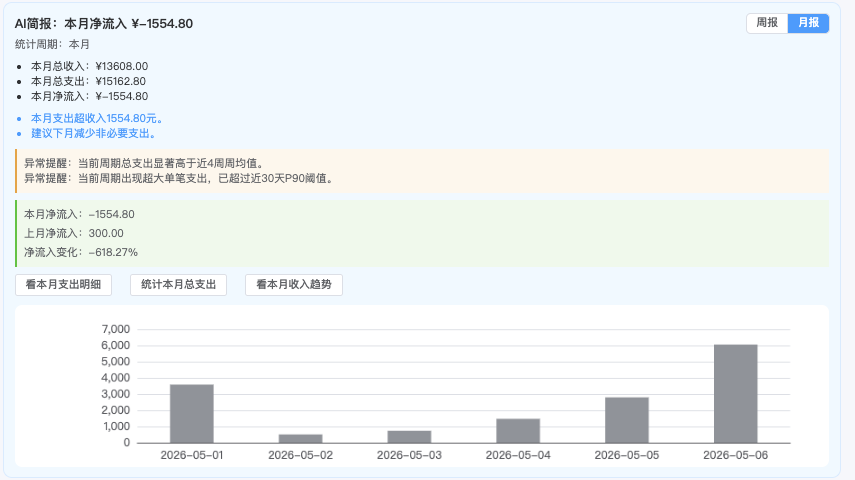
\includegraphics[width=0.92\linewidth]{image/fig-ai-brief-card.png}
    \caption{AI 月报卡片界面图}
\end{figure}

\begin{table}[H]
    \centering
    \caption{AI 周报/月报返回字段说明}
    \label{tab:brief-fields}
    \begin{tabular}{|p{0.25\linewidth}|p{0.65\linewidth}|}
        \hline
        简报字段 & 含义 \\
        \hline
        headline & 简报标题，例如“AI 简报：本月净流入”。 \\
        \hline
        highlights & 本周或本月总收入、总支出、净流入。 \\
        \hline
        comparison & 当前周期与上一周期的收入、支出、净流入对比。 \\
        \hline
        anomalies & 异常支出提醒。 \\
        \hline
        suggestions & AI 生成的简短建议。 \\
        \hline
        quickActions & 可直接点击发送的追问指令。 \\
        \hline
        chartData & 支出趋势图数据。 \\
        \hline
    \end{tabular}
\end{table}

\section{AI 智能转账功能实现}

AI 智能转账对应 transfer 意图，是系统中安全要求最高的 AI 功能。用户可以直接提供银行卡号，也可以使用收款人昵称。例如“向 6222000012345678 转 100 元”会直接提取 toAccountNo 和 amount；“给弟弟转 300 元，备注午餐费”会提取 payeeAlias=弟弟、amount=300、description=午餐费。

handleTransfer 方法首先解析收款账号、收款人昵称、金额、备注和 repeatMode。如果用户没有提供银行卡号但提供了昵称，系统会通过 PayeeContactMapper.selectByUserIdAndAlias 查询当前用户的收款人列表。若未找到昵称，系统提示用户先新增收款人或直接提供银行卡号；若匹配多个收款人，系统提示用户使用更具体昵称。

转账金额解析完成后，系统并不会立即执行扣款，而是调用 accountService.validateTransfer 或 payeeService.validateTransfer 进行校验。校验内容包括参数完整性、金额是否大于 0、付款账户是否存在、收款账户是否存在、账户是否冻结、是否给自己转账以及余额是否充足。校验通过后，系统将转账信息写入 PendingTransfer，并向用户返回脱敏后的确认信息。用户回复“确认”或点击“确认”按钮后，handlePendingTransfer 才会调用真实转账服务执行扣款、收款和流水写入；用户回复“取消”或点击“取消”按钮则删除待确认状态。

 AI 智能转账涉及两轮用户交互和资金操作确认，如图\ref{fig:ai-transfer-flow} 所示，第一轮中用户通过自然语言发起转账，AssistantService 调用 QwenClient 解析 transfer 意图，并根据银行卡号或收款人昵称完成收款人匹配；随后系统调用转账校验服务检查账户状态、余额和自转账等风险条件。校验通过后，系统只生成确认信息并保存 PendingTransfer，不执行资金变动。第二轮中，用户回复“确认”或点击“确认”按钮时系统才调用真实转账服务更新账户余额并写入交易流水；用户回复“取消”或点击“取消”按钮或待确认状态超时则清理 pendingMap，资金操作不会发生。

\begin{figure}[H]
    \centering
    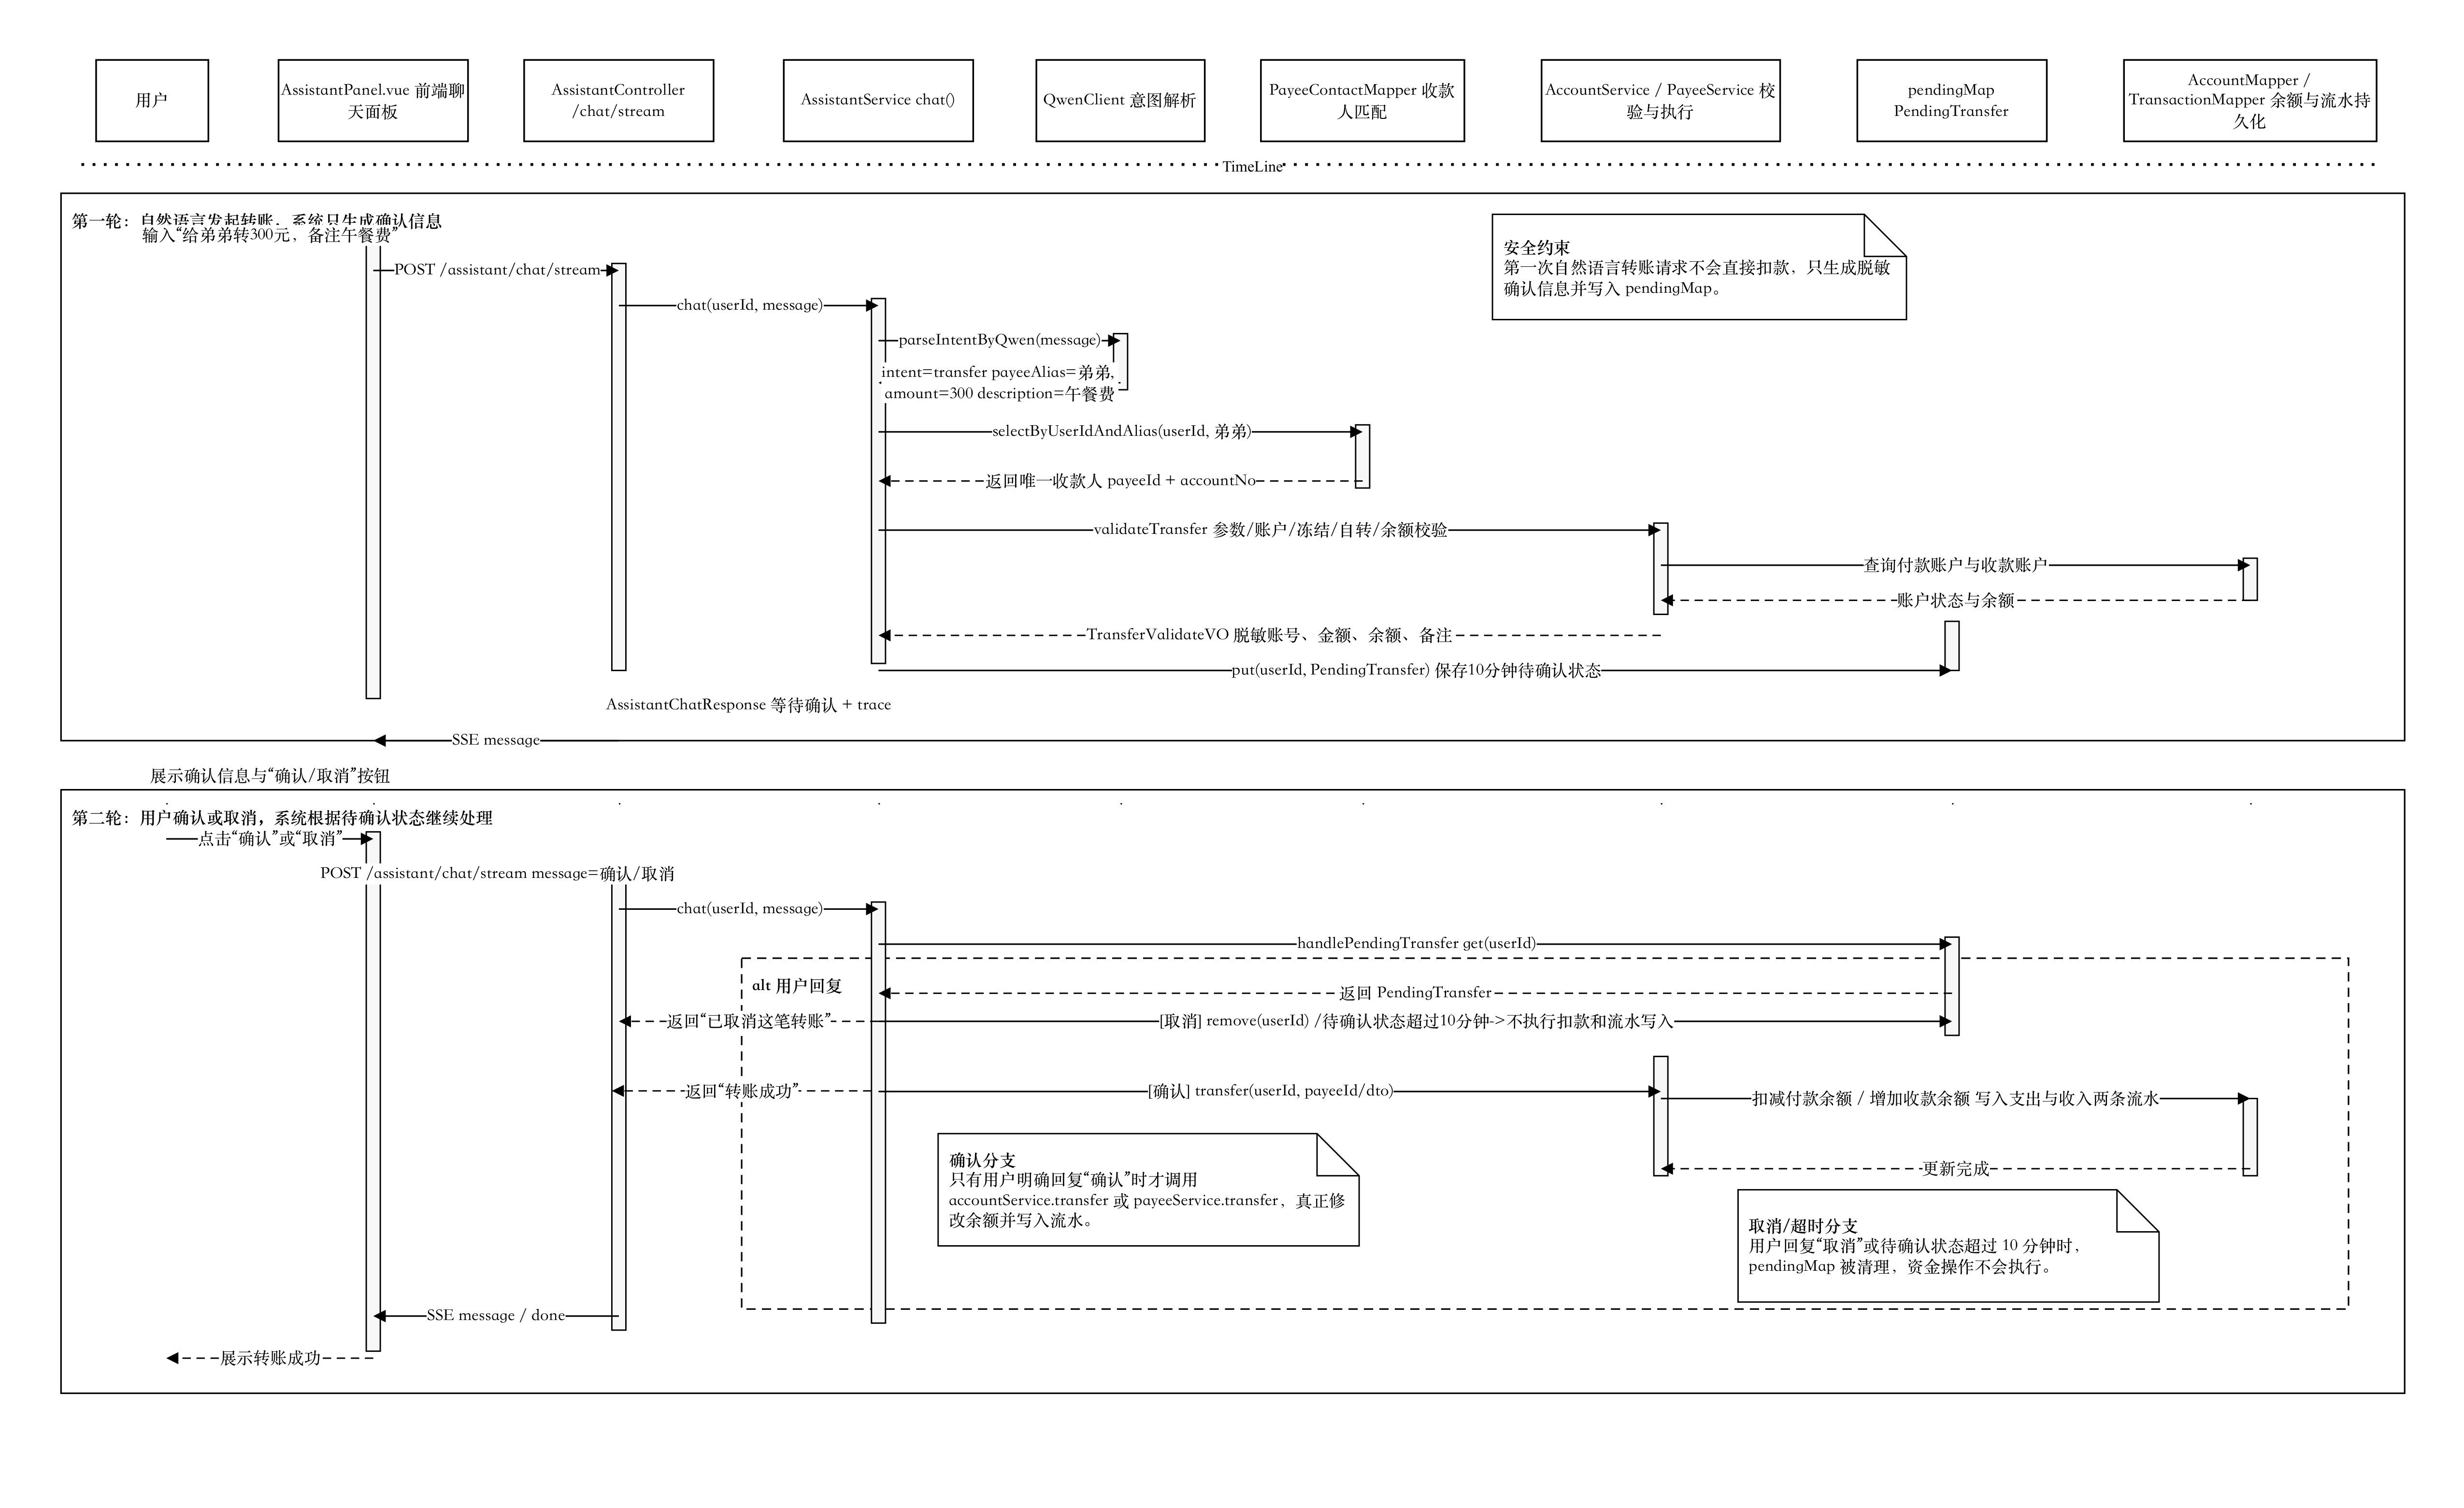
\includegraphics[width=\linewidth]{image/fig-ai-transfer-flow.png}
    \caption{AI 智能转账二次确认时序图}
    \label{fig:ai-transfer-flow}
\end{figure}

\begin{figure}[H]
    \centering
    \IfFileExists{image/fig-ai-transfer-confirm-ui.png}{
        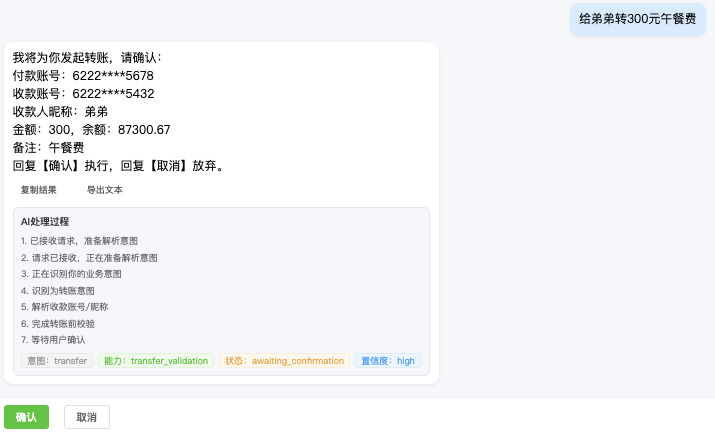
\includegraphics[width=0.92\linewidth]{image/fig-ai-transfer-confirm-ui.png}
    }{
        \fbox{\parbox[c][0.34\linewidth][c]{0.86\linewidth}{\centering 待补充截图：image/fig-ai-transfer-confirm-ui.png}}
    }
    \caption{AI 智能转账二次确认界面图}
    \label{fig:ai-transfer-confirm-ui}
\end{figure}

系统同时实现了历史金额复用能力。当用户输入给弟弟转晚餐费并说明和前天一样时，模型会将 repeatMode 解析为 time\_same，后端根据 Time 工具确定参考时间范围，并通过 selectLatestExpenseByCounterpartyAndDescription 查询该时间范围内同收款人且备注匹配的历史支出流水。若找到记录，系统复用历史金额和备注生成确认信息；若未找到，则提示用户补充转账金额。该能力只解决用户未明确给出金额时的金额补全问题，并不会绕过转账校验和二次确认。

图\ref{fig:reference-transfer-flow} 展示了历史金额复用转账的处理流程。系统首先判断当前 transfer 请求是否属于 amount 为空且包含时间参考的复用场景，然后解析收款人、备注关键词和参考时间范围。查询历史流水时，系统优先查找同收款人、同备注关键词的支出记录；若未找到，再回退查询同收款人的最近支出流水。只有找到真实历史流水时，系统才复用其金额和备注，否则要求用户补充金额。

\begin{figure}[H]
    \centering
    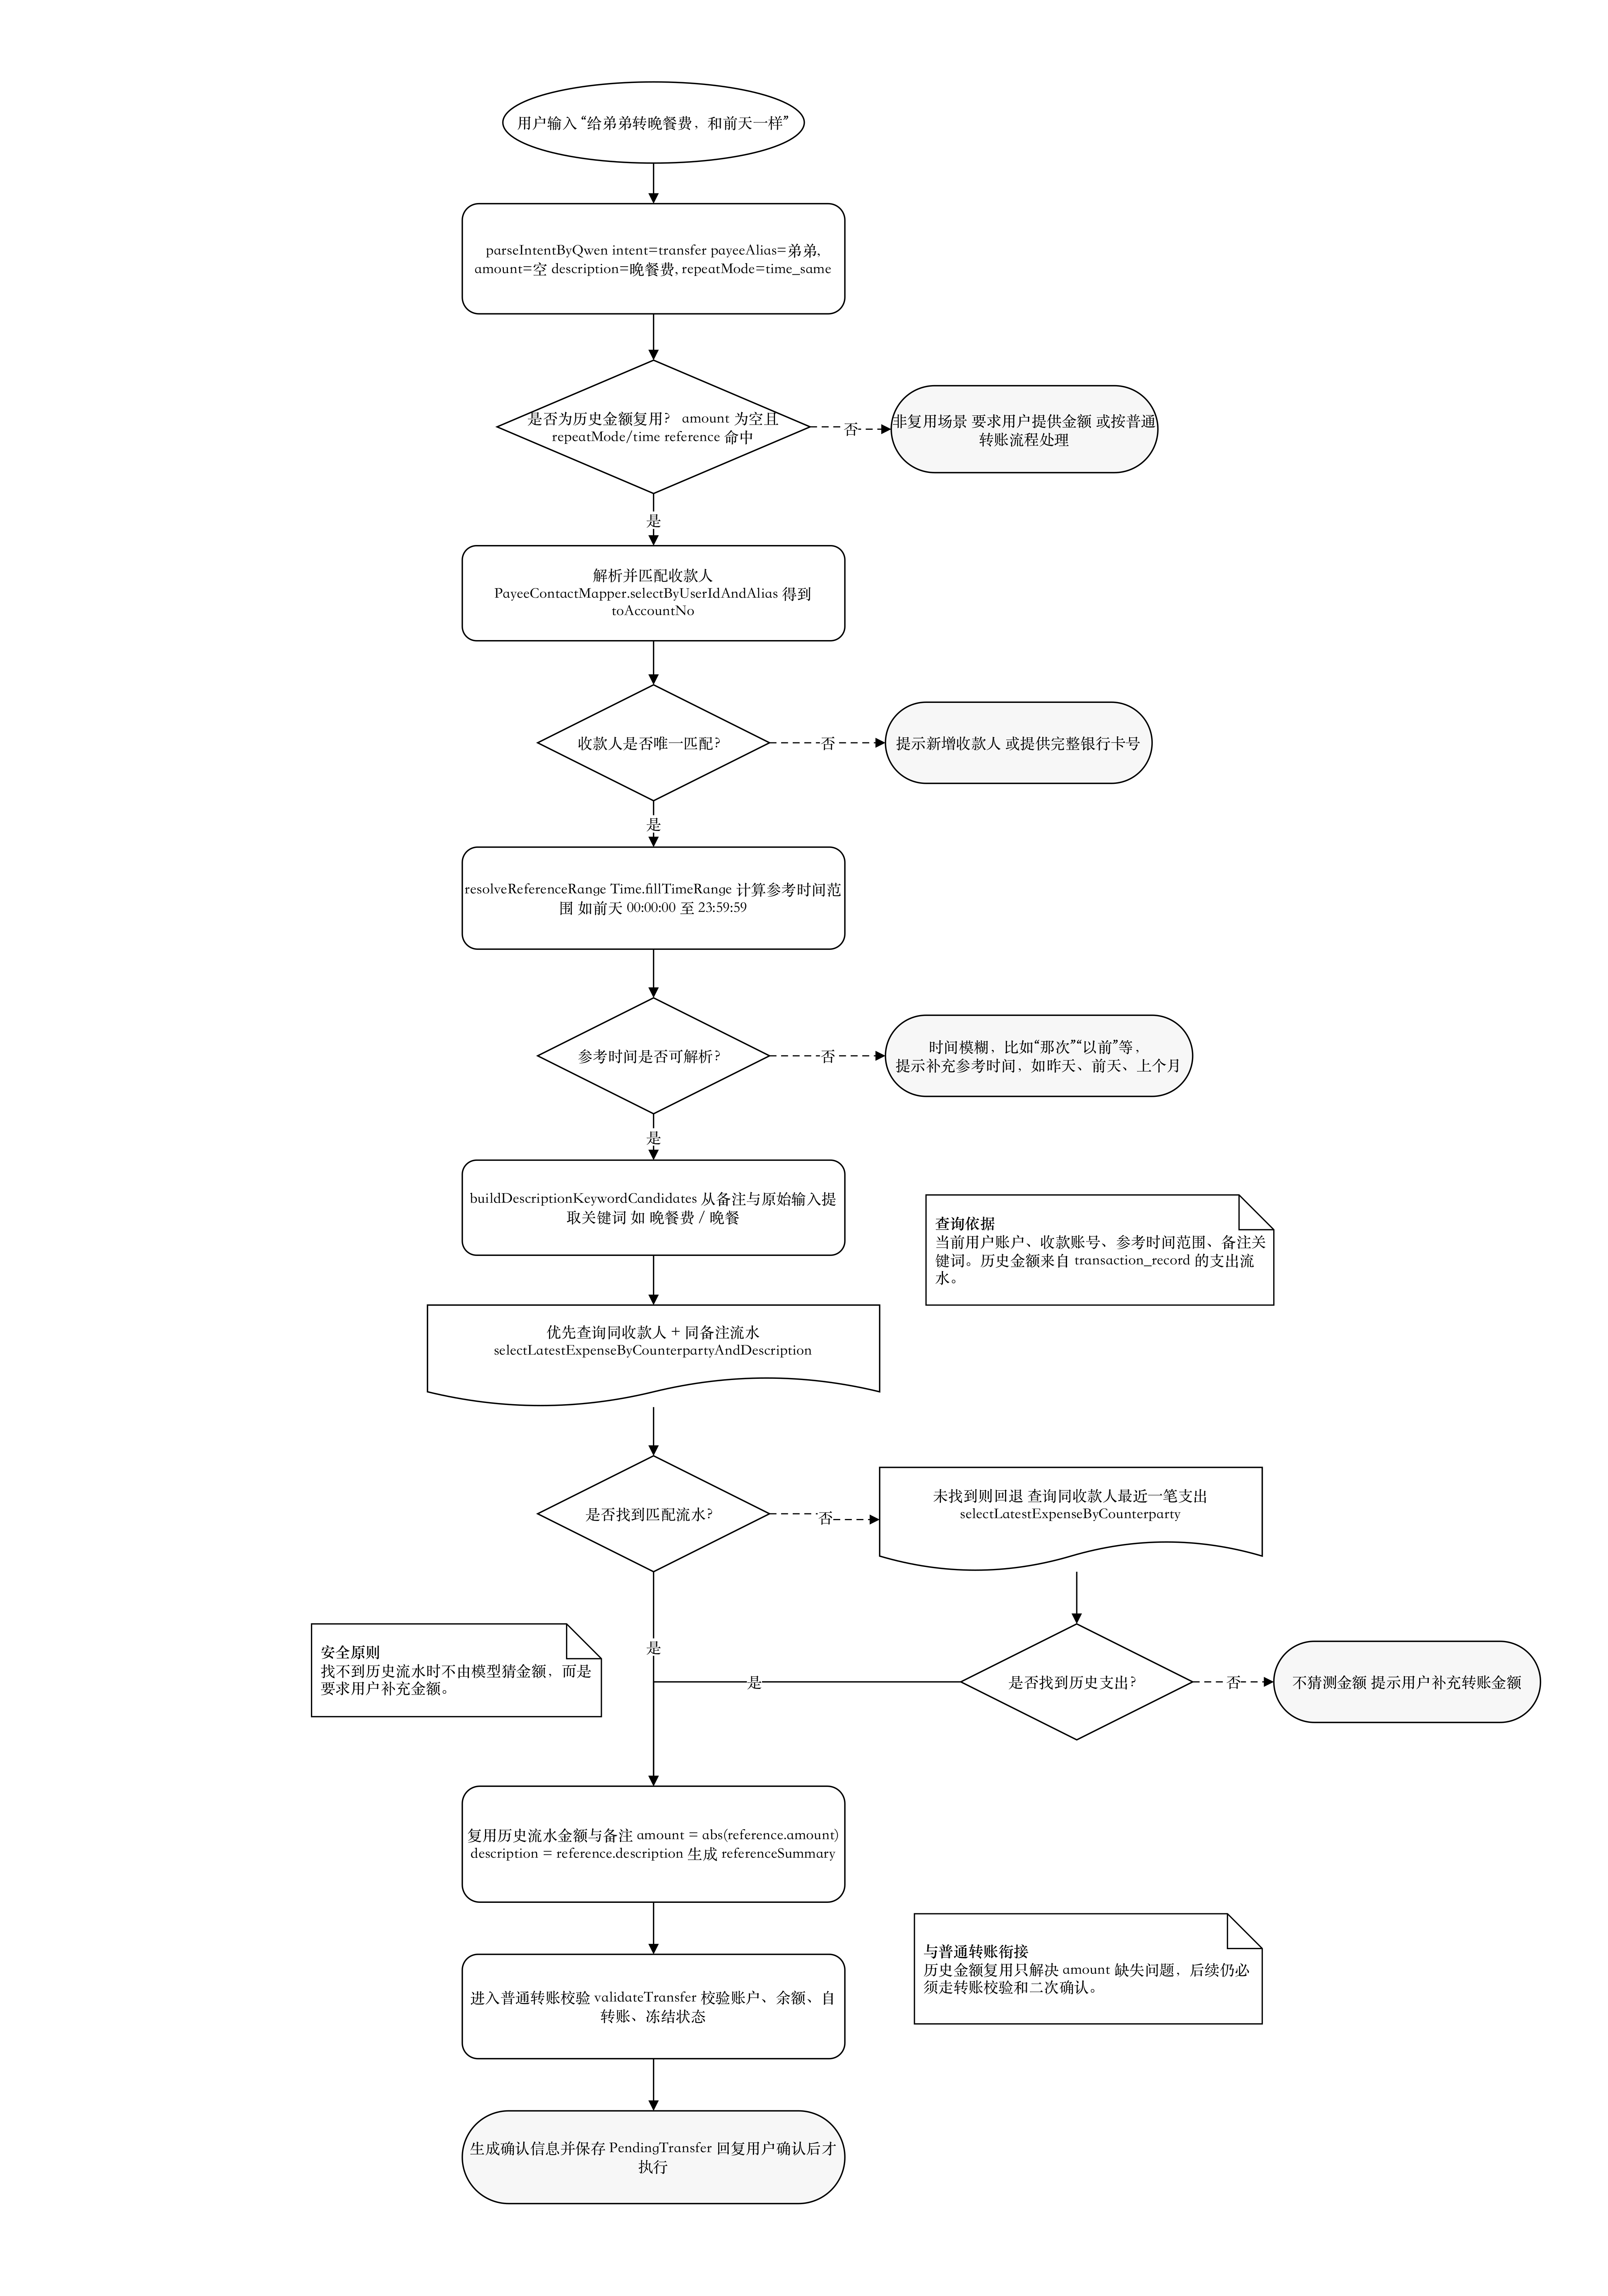
\includegraphics[width=1.00\linewidth]{image/fig-reference-transfer-flow.png}
    \caption{历史金额复用转账流程图}
    \label{fig:reference-transfer-flow}
\end{figure}

\begin{table}[H]
    \centering
    \caption{AI 智能转账安全控制设计}
    \label{tab:transfer-security}
    \begin{tabular}{|p{0.25\linewidth}|p{0.68\linewidth}|}
        \hline
        安全控制点 & 实现方式 \\
        \hline
        收款人确认 & 按银行卡号或收款人昵称解析，昵称不存在或重复时提示用户补充。 \\
        \hline
        账户校验 & 校验付款账户、收款账户是否存在及状态是否正常。 \\
        \hline
        余额校验 & 转账前检查付款账户余额是否充足。 \\
        \hline
        防止自转账 & 付款账号与收款账号相同时抛出业务异常。 \\
        \hline
        二次确认 & AI 首次回复只生成确认信息，用户回复确认后才执行。 \\
        \hline
        账号脱敏 & 确认信息中付款账号和收款账号均以脱敏形式展示。 \\
        \hline
    \end{tabular}
\end{table}

\chapter{系统测试与交互优化分析}

本章对应“可验证评价方式”和“测试与反馈闭环”创新点，重点回答系统实现效果是否能够被数据和测试过程支撑。7.1 说明测试环境、数据来源、能力边界和指标定义；7.2 通过后端自动化测试验证核心服务分支；7.3 验证大模型意图解析和服务分流效果；7.4 通过功能测试、FAQ 检索统计和边界用例验证核心功能；7.5 通过匿名反馈测试日志分析用户体验；7.6 和 7.7 将测试结果回扣到交互优化、效率提升、能力边界和后续改进方向。

\section{测试环境与测试方法}

系统测试以本地开发环境为基础，后端服务运行在 8081 端口，前端通过 Vite 开发服务器代理 /api 请求到后端。数据库使用 MySQL，测试数据来自 sql 目录中的 user、account、payee\_contact 和 transaction\_record 脚本，数据库中数据信息均不涉及真实信息。测试方法以功能测试和交互流程测试为主，重点验证 AI 助手是否能够正确识别用户输入、调用对应业务服务、返回符合预期的文本、图表和确认流程。

本项目测试数据由系统初始化脚本中的虚拟账户、虚拟交易流水、FAQ 初始化数据以及校外企业导师提供的测试建议共同构成。测试过程不使用真实银行客户信息，涉及的账号、姓名、手机号、余额、交易流水和问答内容均为模拟或脱敏数据。交互优化分析重点从功能可用性、任务完成情况和体验反馈角度展开。

测试范围围绕本文定义的 AI 核心功能展开，不将登录、注册、普通页面跳转等基础管理能力作为主要评价对象。测试时首先保证后端服务、数据库和前端代理能够正常启动，然后在 AI 面板中输入典型自然语言指令，观察后端控制台、浏览器界面和接口返回结果是否一致。对于语音输入功能，重点检查识别结果是否能够回填到聊天输入框并继续发送；对于查询类功能，重点检查返回金额、记录条数、交易方向和时间范围是否与数据库样本相符；对于统计类功能，重点检查统计口径、聚合结果、图表数据和导出链接是否完整；对于转账类功能，重点检查系统是否先生成确认信息，是否在用户明确确认前避免直接修改账户余额。

为保证测试结论与源代码一致，本文没有设计超出项目能力范围的测试项。例如，当前系统并未实现商户品类识别和消费场景标签，因此测试只验证系统能否正确拒绝或说明该类请求，而不把这类功能写成已经完成的能力。对于大模型输出具有一定随机性的情况，测试判断以结构化字段和业务服务调用结果为主，而不是要求每次自然语言回复完全相同。这样可以避免把模型措辞差异误判为功能失败，也能更准确地反映系统的真实可用性。

\subsection{测试指标定义与计算方法}

为避免测试结果仅停留在人工描述和表格罗列层面，本文在测试阶段对后端自动化测试、意图识别与服务分流测试、FAQ 知识库检索测试和用户体验测试分别设置量化指标。设某类测试样本集合为
\[
D=\{d_1,d_2,\ldots,d_n\},
\]
其中 \(n\) 表示样本总数。对于第 \(i\) 个测试样本，若系统输出结果与人工期望结果一致，则记为
\[
I_i=
\begin{cases}
1, & \text{系统输出符合预期};\\
0, & \text{系统输出不符合预期}.
\end{cases}
\]
因此，某类测试任务的通过率定义为
\[
P=\frac{\sum_{i=1}^{n} I_i}{n}\times 100\%.
\]
该指标用于功能测试、能力边界测试以及意图识别与服务分流测试中，用于衡量系统在给定测试样本集合上的正确处理比例。

对于后端自动化测试，设测试用例总数为 \(N\)，通过用例数为 \(N_p\)，失败用例数为 \(N_f\)，跳过用例数为 \(N_s\)，则通过率、失败率和跳过率分别定义为
\[
P_{pass}=\frac{N_p}{N}\times 100\%,
\]
\[
P_{fail}=\frac{N_f}{N}\times 100\%,
\]
\[
P_{skip}=\frac{N_s}{N}\times 100\%.
\]
设第 \(k\) 个测试类的执行耗时为 \(t_k\)，测试类数量为 \(m\)，则自动化测试总耗时和平均耗时分别定义为
\[
T_{total}=\sum_{k=1}^{m}t_k,
\]
\[
\bar{T}=\frac{1}{m}\sum_{k=1}^{m}t_k.
\]

对于意图识别与服务分流测试，设第 \(i\) 条测试语句的人工期望分支为 \(y_i\)，系统实际分流结果为 \(\hat{y}_i\)。若二者一致，则认为该样本通过。整体分流准确率定义为
\[
Acc=\frac{1}{n}\sum_{i=1}^{n}\mathbf{1}(\hat{y}_i=y_i)\times 100\%,
\]
其中 \(\mathbf{1}(\cdot)\) 为指示函数，当括号内条件成立时取 1，否则取 0。对于第 \(c\) 类场景，设该类样本数为 \(n_c\)，通过数为 \(p_c\)，则该类场景通过率为
\[
Acc_c=\frac{p_c}{n_c}\times 100\%.
\]

对于 FAQ 知识库检索测试，系统检索结果分为直接命中、相似推荐和未命中三类。设 FAQ 测试问题总数为 \(N_{faq}\)，直接命中数量为 \(N_{hit}\)，相似推荐数量为 \(N_{rec}\)，未命中数量为 \(N_{no}\)，则直接命中率、相似推荐率和未命中率分别为
\[
R_{hit}=\frac{N_{hit}}{N_{faq}}\times 100\%,
\]
\[
R_{rec}=\frac{N_{rec}}{N_{faq}}\times 100\%,
\]
\[
R_{no}=\frac{N_{no}}{N_{faq}}\times 100\%.
\]
对于银行业务相关问题，本文将直接命中和相似推荐均视为有效处理，相关问题覆盖率定义为
\[
R_{cover}=\frac{N_{hit}^{bank}+N_{rec}^{bank}}{N_{bank}}\times 100\%,
\]
其中 \(N_{bank}\) 表示银行业务相关 FAQ 测试样本数量。对于无关问题，若系统进入未命中分支而不是直接编造银行业务答案，则视为有效拦截，无关问题拦截率定义为
\[
R_{reject}=\frac{N_{no}^{irrelevant}}{N_{irrelevant}}\times 100\%.
\]

对于用户体验测试，设第 \(j\) 个任务包含 \(n_j\) 条测试记录。第 \(i\) 条记录的完成状态为 \(c_{ij}\)，完成记为 1，未完成记为 0，则任务完成率定义为
\[
C_j=\frac{\sum_{i=1}^{n_j}c_{ij}}{n_j}\times 100\%.
\]
设第 \(i\) 条记录的响应耗时为 \(d_{ij}\)，单位为毫秒，则第 \(j\) 个任务的平均响应耗时为
\[
\bar{T}_j=\frac{1}{n_j}\sum_{i=1}^{n_j}\frac{d_{ij}}{1000}.
\]
设第 \(i\) 条记录的操作步数为 \(s_{ij}\)，则第 \(j\) 个任务的平均操作步数为
\[
\bar{S}_j=\frac{1}{n_j}\sum_{i=1}^{n_j}s_{ij}.
\]
对于理解度、满意度、安全感和语言表达四项主观评分，评分范围均为 1--5 分。设第 \(i\) 条记录在第 \(q\) 个评分维度上的分值为 \(r_{ijq}\)，则第 \(j\) 个任务在该维度上的平均评分为
\[
\bar{R}_{jq}=\frac{1}{n_j}\sum_{i=1}^{n_j}r_{ijq}.
\]
分值越高，表示测试者对该任务的理解程度、满意程度、安全感或语言表达认可程度越高。

\section{后端自动化测试与指标记录}

为弥补单纯人工体验测试样本量较小、数据来源不够稳定的问题，本文补充了 JUnit 5 和 Mockito 自动化测试。测试不直接连接真实大模型服务和真实银行数据库，而是通过 Mock 对象构造固定返回值，从而重点验证业务分支、参数解析、知识库检索和日志记录逻辑。这样可以在每次代码修改后重复执行相同用例，避免只依赖一次性人工操作截图或主观反馈。

自动化测试覆盖范围如表 \ref{tab:backend-auto-test-scope} 所示。测试重点不是证明系统已经具备生产级稳定性，而是验证论文中描述的核心后端逻辑确实存在，并能够在可控输入下得到预期输出。

\begin{table}[H]
    \centering
    \caption{后端自动化测试覆盖范围}
    \label{tab:backend-auto-test-scope}
    \small
    \setlength{\tabcolsep}{3pt}
    \begin{tabular}{|p{0.18\linewidth}|p{0.22\linewidth}|p{0.37\linewidth}|p{0.08\linewidth}|p{0.07\linewidth}|}
        \hline
        测试对象 & 测试类简称 & 覆盖内容 & 用例数 & 结果 \\
        \hline
        应用入口 & 应用启动测试 & 应用主类可构造，避免基础类加载失败。 & 1 & 通过 \\
        \hline
        时间解析 & 时间工具测试 & 本月范围、最近天数范围、昨天等自然语言时间归一化。 & 3 & 通过 \\
        \hline
        统计服务 & 统计服务测试 & 支出合计、趋势列表、空结果处理。 & 3 & 通过 \\
        \hline
        转账校验 & 账户服务测试 & 正常转账校验、余额不足、向本人转账拦截。 & 3 & 通过 \\
        \hline
        FAQ 检索 & 知识库测试 & 直接命中、相似推荐、未命中、查询日志写入。 & 4 & 通过 \\
        \hline
        AI 编排流程 & 助手服务测试 & 情绪安抚、余额查询、FAQ 问答、转账取消、多轮补全。 & 5 & 通过 \\
        \hline
        指标日志 & 日志服务测试 & trace 信息提取、日志表不可用时不影响主流程。 & 2 & 通过 \\
        \hline
        合计 & -- & 覆盖 AI 助手主要后端分支。 & 21 & 通过 \\
        \hline
    \end{tabular}
\end{table}

测试命令为 mvn test，测试报告由 Maven Surefire 插件生成。2026 年 4 月 30 日在本地环境执行结果如表 \ref{tab:backend-auto-test-result} 所示。表中“用例耗时”为 Surefire 报告中各测试类 time 字段的合计或单项值，Maven 构建总耗时还包含依赖解析、编译和测试框架启动时间。

\begin{table}[H]
    \centering
    \caption{后端自动化测试执行结果}
    \label{tab:backend-auto-test-result}
    \small
    \setlength{\tabcolsep}{4pt}
    \begin{tabular}{|p{0.42\linewidth}|p{0.12\linewidth}|p{0.12\linewidth}|p{0.12\linewidth}|p{0.12\linewidth}|}
        \hline
        测试类简称 & 用例数 & 失败数 & 跳过数 & 耗时/s \\
        \hline
        应用启动测试 & 1 & 0 & 0 & 0.084 \\
        \hline
        时间工具测试 & 3 & 0 & 0 & 0.304 \\
        \hline
        统计服务测试 & 3 & 0 & 0 & 1.693 \\
        \hline
        账户服务测试 & 3 & 0 & 0 & 0.101 \\
        \hline
        日志服务测试 & 2 & 0 & 0 & 0.523 \\
        \hline
        知识库测试 & 4 & 0 & 0 & 0.086 \\
        \hline
        助手服务测试 & 5 & 0 & 0 & 0.733 \\
        \hline
        合计 & 21 & 0 & 0 & 3.524 \\
        \hline
    \end{tabular}
\end{table}

根据上述自动化测试指标定义，本次后端自动化测试共执行 21 个用例，其中通过 21 个，失败和跳过均为 0。因此自动化测试通过率为
\[
P_{pass}=\frac{21}{21}\times 100\%=100.0\%,
\]
失败率和跳过率均为
\[
P_{fail}=P_{skip}=0.
\]
各测试类耗时相加得到总耗时
\[
T_{total}=0.084+0.304+1.693+0.101+0.523+0.086+0.733=3.524s.
\]

\begin{figure}[H]
    \centering
    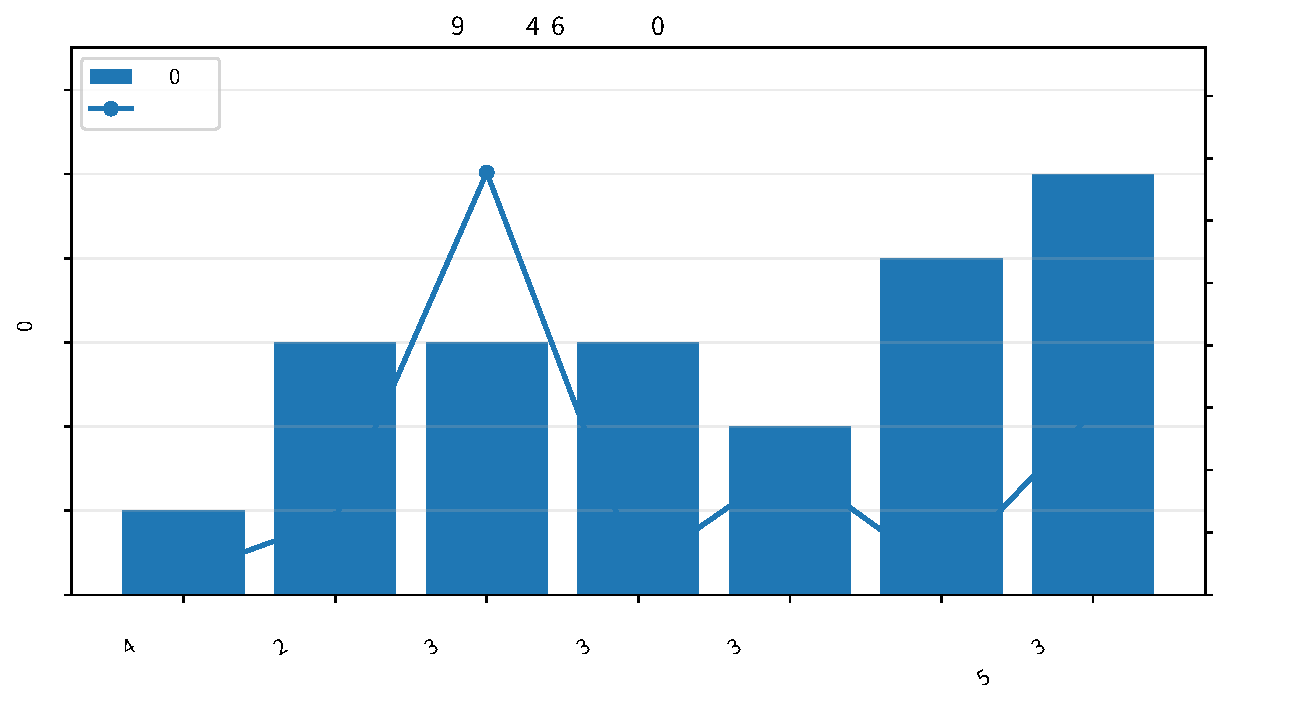
\includegraphics[width=0.9\linewidth]{image/fig_7_3_backend_test_cases_time.pdf}
    \caption{后端自动化测试用例数与耗时对比}
    \label{fig:backend-test-cases-time}
\end{figure}

从图 \ref{fig:backend-test-cases-time}可以看出，助手服务测试和知识库测试覆盖用例数相对较多，统计服务测试耗时最高。各测试类均未出现失败和跳过情况，说明后端核心分支能够在可控输入下稳定通过。

除测试报告外，后端还增加了assistant\_test\_log 指标日志表，用于记录 AI 助手请求的运行结果。主要字段中，duration\_ms 可用于统计接口处理耗时，success、result\_code 和 biz\_code 可用于统计成功率和异常类型，intent 可用于记录系统实际识别出的业务意图，trace\_tool 和 trace\_status 可用于分析系统实际调用的是余额查询、流水查询、统计服务、FAQ 检索还是转账确认流程。为支撑匿名反馈测试模块，表中还扩展 test\_session\_id、participant\_code、task\_code、task\_name、completed、operation\_steps、understanding\_score、satisfaction\_score、safety\_score、language\_score 和 user\_feedback 等可用性测试字段，这些字段只有在进入匿名测试反馈环节才会记录，其中 task\_code 和 task\_name 来自前端匿名反馈测试入口中的 U1--U8 任务选择，operation\_steps 只记录前端可以观察到的关键动作，如选择任务、填入示例、启动语音输入、发送消息以及转账确认或取消，不记录无法准确观测的键盘输入字符数。四类评分字段采用 1--5 的整数值，并随每条测试任务聊天记录写入，而不是只在测试结束时记录一次总体评分。

该日志表的作用是把用户体验测试中的“完成时间、是否成功、调用路径是否正确”等观察项转化为后端可记录字段。人工测试仍然用于观察用户是否理解回复、是否愿意继续使用等具体反馈的问题；自动化测试和日志表则用于补充客观证据，说明测试数据可以从可重复执行的测试报告和后端运行记录中得到，而不是仅依赖主观描述。

\section{意图识别准确性测试}

为了验证本文所选择的“大语言模型意图解析 + FAQ 检索 + 规则化后备处理 + 情绪关键词检测”方案是否能够满足任务书中“选择适用的技术和算法”的要求，本文对 AssistantService 的意图识别和分流链路进行了测试。需要说明的是，AssistantService 中的大模型解析方法 parseIntentByQwen 只要求模型输出 balance、transactions、statistics、transfer 和 other 五类基础意图类型；FAQ 咨询、异常情绪安抚和待确认状态处理并不是模型直接输出的新意图类型，而是在服务编排层继续分流得到的处理结果。

从源码流程看，用户请求进入 AssistantService 后，系统先处理待确认转账和待补全流水查询，再通过 handleEmotionSupport 对明显投诉、愤怒或焦虑表达进行关键词检测；如果上述规则未命中，系统才调用 parseIntentByQwen 进行基础意图解析。对于 FAQ 咨询、未实现能力和非银行业务问题，模型层统一输出 other，随后由 handleFaqOrFallback 进入 FAQ 知识库检索或后备回复。因此，本节测试不仅记录模型层意图字段是否正确，也记录最终 trace 中的工具调用和状态是否符合预期。

测试样本覆盖余额查询、流水查询、账单统计、转账发起、FAQ 咨询、异常情绪安抚、不支持能力拦截和多轮状态处理八类场景，每类选取 10 条中文自然语言表达，共 80 条。样本既包含直接表达，如“查一下我的余额”“统计这个月总支出”，也包含口语化表达，如“我现在账户里还有多少钱”“最近几天的交易明细给我看看”“给弟弟转晚餐费，和昨天一样”。FAQ 咨询样本包括“卡丢了怎么挂失”“跨行转账要多久”等常见问题；情绪后备处理样本包括“我很生气，我要投诉”“我有点担心这笔钱”等表达；不支持能力样本包括“按消费场景标签统计一下”“按商户类型分析消费”等超出当前系统能力边界的问题。

\begin{table}[H]
    \centering
    \caption{AI 助手意图与分流测试结果}
    \label{tab:intent-recognition-test}
    \scriptsize
    \setlength{\tabcolsep}{2pt}
    \begin{tabular}{|p{0.13\linewidth}|p{0.2\linewidth}|p{0.1\linewidth}|p{0.1\linewidth}|p{0.1\linewidth}|p{0.27\linewidth}|}
        \hline
        场景类型 & 期望处理分支 & 测试语句数 & 通过数 & 通过率 & 典型测试语句 \\
        \hline
        查余额 & balance / account\_info & 10 & 10 & 100.0\% & 查一下我的余额 \\
        \hline
        查流水 & transactions / transaction\_query & 10 & 9 & 90.0\% & 查最近5条支出记录 \\
        \hline
        账单统计 & statistics / statistics\_service & 10 & 9 & 90.0\% & 最近7天我花了多少钱 \\
        \hline
        转账发起 & transfer / transfer\_validation & 10 & 9 & 90.0\% & 给弟弟转300元午餐费 \\
        \hline
        FAQ 咨询 & other 后进入 faq\_knowledge\_base & 10 & 10 & 100.0\% & 卡丢了怎么挂失 \\
        \hline
        情绪安抚 & emotion\_support / rule\_emotion & 10 & 10 & 100.0\% & 我很生气，我要投诉 \\
        \hline
        不支持能力 & other / qwen\_fallback & 10 & 9 & 90.0\% & 按消费场景标签统计一下 \\
        \hline
        多轮与确认状态 & pending 状态续接或取消 & 10 & 10 & 100.0\% & 1月；确认；取消 \\
        \hline
        合计 & -- & 80 & 76 & 95.0\% & 典型样本集合 \\
        \hline
    \end{tabular}
\end{table}

根据意图识别与服务分流准确率公式，本次测试共构造 80 条典型样本，其中 76 条样本的实际分流结果与人工期望一致，因此整体分流准确率为
\[
Acc=\frac{76}{80}\times 100\%=95.0\%.
\]
其中查流水、账单统计、转账发起和不支持能力拦截场景的单类通过率为 90.0\%，余额查询、FAQ 咨询、情绪安抚和多轮确认场景的单类通过率为 100.0\%。

\begin{figure}[H]
    \centering
    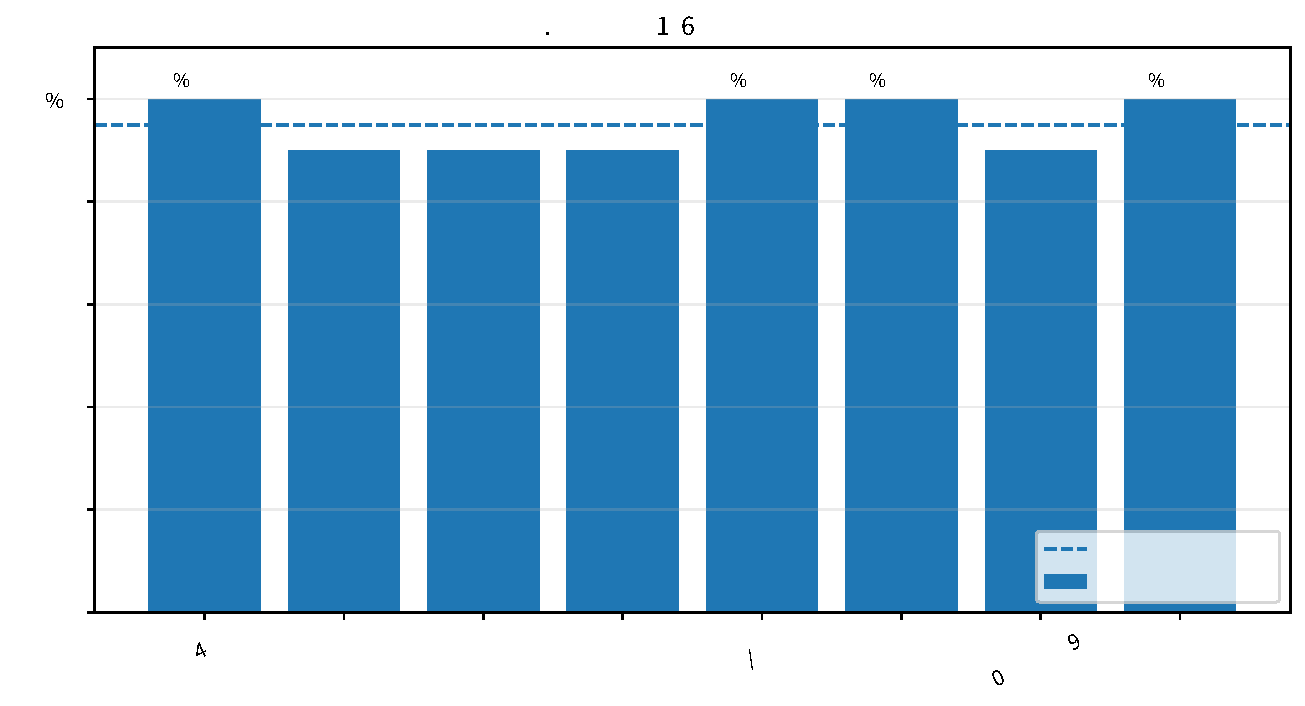
\includegraphics[width=0.88\linewidth]{image/fig_7_4_intent_routing_pass_rate.pdf}
    \caption{AI 助手意图与分流测试通过率}
    \label{fig:intent-routing-pass-rate}
\end{figure}

图 \ref{fig:intent-routing-pass-rate} 展示了不同场景下 AI 助手意图识别与服务分流的通过率。余额查询、FAQ 咨询、情绪安抚以及多轮确认类场景均达到 100.0\%，查流水、账单统计、转账发起和不支持能力拦截场景为 90.0\%。这说明系统在高频和边界明确的场景中表现较稳定，而模糊表达和超出能力边界的请求仍是后续优化重点。结合表 \ref{tab:intent-recognition-test} 可知，本次 80 条典型测试样本中系统通过 76 条，综合通过率为 95.0\%。未通过样例及原因如表 \ref{tab:intent-error-samples} 所示。

\begin{table}[H]
    \centering
    \caption{AI 助手意图与分流误判样例}
    \label{tab:intent-error-samples}
    \scriptsize
    \setlength{\tabcolsep}{2pt}
    \begin{tabular}{|p{0.22\linewidth}|p{0.14\linewidth}|p{0.17\linewidth}|p{0.24\linewidth}|p{0.13\linewidth}|}
        \hline
        测试样例 & 人工期望分支 & 实际模型或分流结果 & 问题原因 & 优化方向 \\
        \hline
        最近几天花钱情况给我看看 & statistics & transactions & “花钱情况”既可理解为支出明细，也可理解为支出汇总，语义边界不够明确。 & 提示词强调“花钱情况、消费情况”优先进入统计。 \\
        \hline
        查一下这个月比较大的几笔收入 & transactions & statistics & “比较大的”触发了最大值统计倾向，但用户实际希望查看多条收入流水。 & 增加“大几笔、几条记录”优先流水查询规则。 \\
        \hline
        给弟弟转晚餐费，和那天一样 & transfer & other & “那天一样”缺少明确日期，历史金额复用所需的参考时间不完整。 & 增加追问日期逻辑和 repeatMode 示例。 \\
        \hline
        按吃饭购物场景统计一下本月支出 & other / qwen\_fallback & statistics & 当前系统没有消费场景标签字段，但模型容易把“统计”关键词识别为已支持统计。 & 扩展不支持能力关键词和后置拦截规则。 \\
        \hline
    \end{tabular}
\end{table}

测试结果说明，在本文设定的银行客服功能边界内，使用大语言模型进行基础意图解析，再配合 FAQ 知识库、关键词规则和状态机后备处理，能够满足原型系统的基本需求。误判主要出现在用户表达较模糊、同时包含多个业务关键词或请求超出系统能力边界的场景。例如，“花钱情况”可能在流水明细和支出统计之间摇摆；“比较大的几笔收入”可能在多条流水和最大值统计之间摇摆；“吃饭购物场景”虽然是用户常见表达，但当前数据库没有对应标签字段，仍需要依靠 containsUnsupportedScope 和后置规则继续拦截。该结果也说明，本文系统不是把所有请求都交给大模型自由处理，而是通过后端编排层将 FAQ、情绪安抚和风险操作确认纳入更可控的分流链路。

需要说明的是，该结果并不表示系统能够对任意开放式自然语言问题都保持同等识别准确率。本次测试样本主要围绕系统已实现功能和答辩演示高频问法构造，样本构成见附录 \ref{app:test-samples}，目的是验证项目源码中已设计的意图解析提示词、JSON 输出约束、FAQ 分流、情绪关键词检测、状态续接和不支持能力拦截是否有效。测试样本由系统已实现功能边界内的典型问法构成，因此该结果不能外推为开放域自然语言理解准确率。对于更大规模真实用户语料，仍需要继续扩大样本数量，并引入准确率、召回率、混淆矩阵和人工复核等更完整的评估方法。

\section{功能测试}

\begin{table}[H]
    \centering
    \caption{AI 核心功能测试用例表}
    \label{tab:test-cases}
    \begin{tabular}{|p{0.1\linewidth}|p{0.28\linewidth}|p{0.42\linewidth}|p{0.1\linewidth}|}
        \hline
        编号 & 测试输入或操作 & 预期结果 & 结论 \\
        \hline
        T1 & 输入“查一下我的余额” & 识别为 balance，返回账户信息和余额。 & 通过 \\
        \hline
        T2 & 输入“查最近 5 条支出记录” & 识别为 transactions，返回支出流水列表。 & 通过 \\
        \hline
        T3 & 输入“查 17 号收入记录”后回复“1 月” & 系统先追问月份，再查询指定日期收入流水。 & 通过 \\
        \hline
        T4 & 输入“统计这个月总支出” & 识别为 statistics，返回支出总额、统计口径和导出链接。 & 通过 \\
        \hline
        T5 & 输入“看最近 7 天支出趋势” & 返回趋势图数据，前端可渲染柱状图或折线图。 & 通过 \\
        \hline
        T6 & 打开 AI 面板 & 自动加载周报或月报卡片。 & 通过 \\
        \hline
        T7 & 输入“给弟弟转 300 元，备注午餐费” & 按昵称匹配收款人并返回转账确认信息。 & 通过 \\
        \hline
        T8 & 在待确认转账状态下输入“取消” & 取消转账并清除待确认状态。 & 通过 \\
        \hline
        T9 & 输入“给弟弟转晚餐费，和昨天一样” & 识别为 transfer，按昵称匹配收款人，并根据历史流水复用金额和备注，生成待确认转账信息。 & 通过 \\
        \hline
        T10 & 提出消费分类或商户类型分析请求 & 系统说明当前不支持该类能力。 & 通过 \\
        \hline
        T11 & 点击语音输入按钮并说出“查一下我的余额” & 浏览器完成语音转写，输入框出现识别文本，发送后进入余额查询流程。 & 通过 \\
        \hline
        T12 & 输入“我很生气，我要投诉” & 系统识别异常情绪或投诉表达，先进行安抚，并提示拨打虚拟客服电话 010-1234-5678 联系人工客服。 & 通过 \\
        \hline
        T13 & 输入“卡丢了怎么挂失” & 系统进入 FAQ 知识库检索，命中银行卡挂失问题并返回标准答案。 & 通过 \\
        \hline
        T14 & 输入“转账有问题” & 系统未直接确定唯一答案时，返回转账相关的相似问题推荐。 & 通过 \\
        \hline
    \end{tabular}
\end{table}

为进一步验证系统不会把未实现能力或高风险操作包装成正常结果，本文补充了能力边界与安全回退测试，如表 \ref{tab:boundary-test} 所示。该表重点观察系统在无法回答、不能执行或需要用户确认时，是否能够进入明确的拒答、推荐、追问、取消或安抚分支。

\begin{table}[H]
    \centering
    \caption{AI 能力边界与安全回退测试}
    \label{tab:boundary-test}
    \scriptsize
    \setlength{\tabcolsep}{2pt}
    \begin{tabular}{|p{0.21\linewidth}|p{0.31\linewidth}|p{0.3\linewidth}|p{0.08\linewidth}|}
        \hline
        测试输入或场景 & 预期边界行为 & 实现机制 & 结论 \\
        \hline
        按消费场景标签统计本月支出 & 不生成虚假的分类统计结果，提示当前不支持该能力。 & containsUnsupportedScope 拦截消费分类、品类、商户类型和场景标签类请求。 & 通过 \\
        \hline
        今天西安天气怎么样 & 不编造银行业务答案，进入 FAQ 未命中或后备回复。 & FAQ 检索 no\_answer 后进入 fallbackChat，并限制回答范围。 & 通过 \\
        \hline
        卡丢了怎么挂失 & 不由模型自由编写银行规则，优先返回知识库标准答案。 & handleFaqOrFallback 调用 faq\_knowledge 表，并写入 faq\_query\_log。 & 通过 \\
        \hline
        给弟弟转 300 元午餐费 & 不直接扣款，只生成待确认转账信息。 & handleTransfer 完成收款人匹配和校验后写入 pendingMap，等待确认。 & 通过 \\
        \hline
        待确认转账后输入“取消” & 清除待确认状态，不继续执行资金操作。 & handlePendingTransfer 识别取消意图并移除 pendingMap。 & 通过 \\
        \hline
        我很生气，我要投诉 & 不继续普通业务闲聊，先安抚并引导人工客服。 & handleEmotionSupport 在调用模型前进行关键词检测。 & 通过 \\
        \hline
    \end{tabular}
\end{table}

从测试结果看，系统能够覆盖论文设计的语音输入、FAQ 知识库问答、异常情绪安抚和五项核心 AI 业务功能。对于语音输入任务，系统能够把用户语音转换为可编辑文本；对于 FAQ 咨询问题，系统能够从知识库中返回标准答案或相似问题推荐；对于异常情绪或投诉表达，系统能够先安抚用户并提示人工客服渠道；对于常规查询类任务，系统能够通过意图解析进入对应业务流程；对于缺失信息的查询，系统能够通过多轮对话补全；对于转账类任务，系统能够在执行前给出确认信息并等待用户明确操作。

语音输入测试主要验证前端输入入口。用户点击语音输入按钮后，浏览器请求麦克风权限并启动 SpeechRecognition。识别到中文语音后，前端将转写文本回填到 chatInput 中，用户可继续修改或直接发送。该测试说明语音识别已经接入智能客服交互入口，但其后续业务处理仍然遵循文本请求链路，不会绕过后端意图解析和安全校验。

异常情绪安抚测试主要验证客服交互边界。用户输入明显包含投诉、愤怒或焦虑的表达时，后端先触发 handleEmotionSupport 方法，返回安抚话术和人工客服电话，而不是继续进入普通业务意图解析。测试表明，该模块能够对明显负面情绪进行基础识别，并将复杂服务纠纷引导到人工客服渠道。由于该模块不参与账户和转账业务执行，因此不会改变系统的资金安全边界。

FAQ 知识库测试主要验证常见咨询问题是否能够从数据库返回确定答案。用户输入“卡丢了怎么挂失”“跨行转账要多久”“验证码收不到怎么办”等问题时，系统先进入 FAQ 检索流程，命中后返回 faq\_knowledge 表中的标准答案；对于“转账有问题”等较模糊表达，系统返回相似问题推荐；对于明显无关问题，系统记录 no\_answer 后再进入后备回复。通过 faq\_query\_log 表可以统计命中数量、推荐数量和未命中数量，使实验部分不只停留在“通过/不通过”的描述。

为进一步验证 FAQ 知识库模块的实际效果，本文从知识库测试集中选取银行卡业务、转账业务、密码与安全、贷款咨询和无关问题五类样本，每类 10 条，共 50 条问题进行检索测试。测试结果按 faq\_query\_log 中的 result\_type 字段统计，结果如表 \ref{tab:faq-knowledge-stat} 所示。

\begin{table}[H]
    \centering
    \caption{FAQ 知识库检索统计结果}
    \label{tab:faq-knowledge-stat}
    \small
    \setlength{\tabcolsep}{3pt}
    \begin{tabular}{|p{0.16\linewidth}|p{0.12\linewidth}|p{0.12\linewidth}|p{0.12\linewidth}|p{0.12\linewidth}|p{0.26\linewidth}|}
        \hline
        测试类别 & 测试问题数 & 直接命中 & 相似推荐 & 未命中 & 说明 \\
        \hline
        银行卡业务 & 10 & 8 & 2 & 0 & 挂失、补卡、吞卡、交易提醒等。 \\
        \hline
        转账业务 & 10 & 7 & 3 & 0 & 到账时间、失败原因、限额、填错账号等。 \\
        \hline
        密码与安全 & 10 & 8 & 1 & 1 & 密码找回、验证码、诈骗防范、异常交易等。 \\
        \hline
        贷款咨询 & 10 & 7 & 2 & 1 & 贷款材料、进度、提前还款、利率和逾期等。 \\
        \hline
        无关问题 & 10 & 0 & 1 & 9 & 天气、机票、外卖、旅游、论文格式等。 \\
        \hline
        合计 & 50 & 30 & 9 & 11 & 相关问题优先返回答案或推荐，无关问题避免直接编造答案。 \\
        \hline
    \end{tabular}
\end{table}

根据 FAQ 检索指标定义，本次 FAQ 测试共 50 条样本，其中直接命中 30 条，相似推荐 9 条，未命中 11 条，因此直接命中率、相似推荐率和未命中率分别为
\[
R_{hit}=\frac{30}{50}\times 100\%=60.0\%,
\]
\[
R_{rec}=\frac{9}{50}\times 100\%=18.0\%,
\]
\[
R_{no}=\frac{11}{50}\times 100\%=22.0\%.
\]
在 40 条银行业务相关问题中，直接命中 30 条，相似推荐 8 条，因此相关问题覆盖率为
\[
R_{cover}=\frac{30+8}{40}\times 100\%=95.0\%.
\]
在 10 条无关问题中，9 条进入未命中分支，因此无关问题拦截率为
\[
R_{reject}=\frac{9}{10}\times 100\%=90.0\%.
\]

\begin{figure}[H]
    \centering
    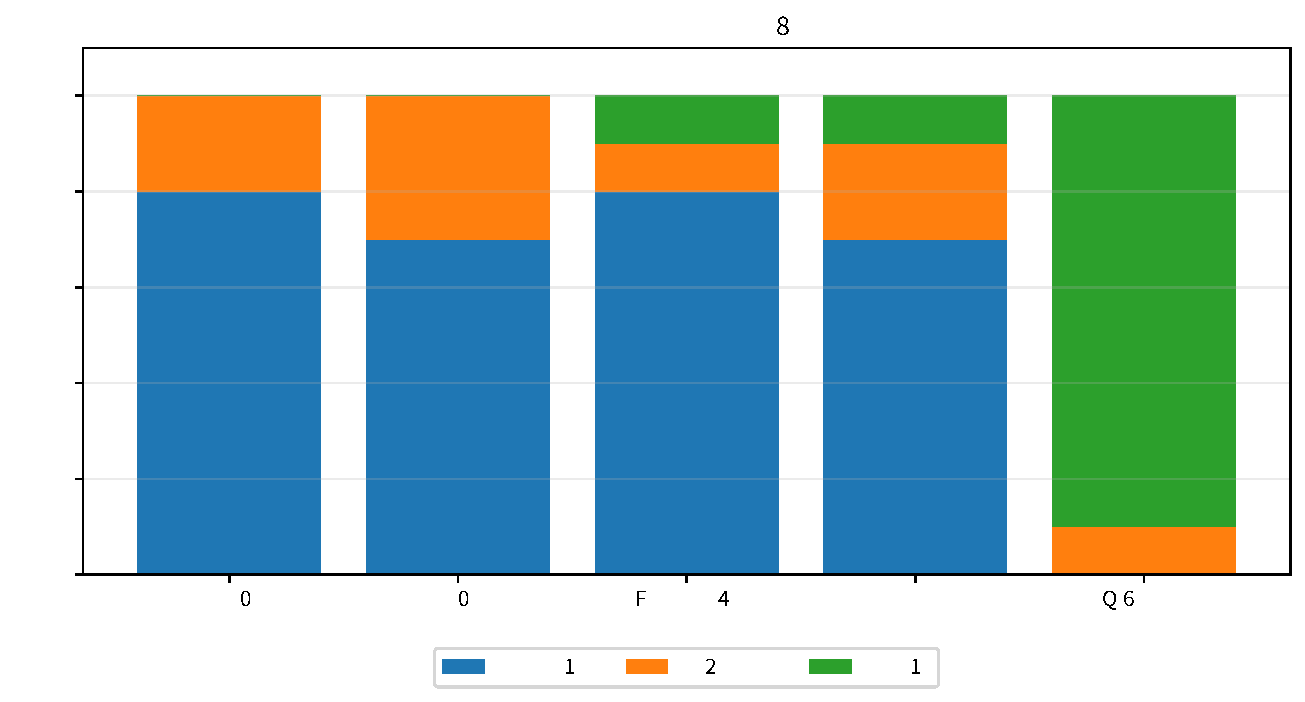
\includegraphics[width=0.88\linewidth]{image/fig_7_5_faq_retrieval_distribution.pdf}
    \caption{FAQ 知识库检索结果分布}
    \label{fig:faq-retrieval-distribution}
\end{figure}

从图 \ref{fig:faq-retrieval-distribution} 可以看出，银行卡业务、转账业务、密码与安全、贷款咨询等银行相关问题主要进入直接命中或相似推荐分支，而无关问题大部分进入未命中分支。该结果说明 FAQ 知识库既能补充常见咨询问答，也能在一定程度上避免系统对非银行问题直接编造答案。结合表 \ref{tab:faq-knowledge-stat} 可知，在 40 条银行业务相关 FAQ 样本中，系统直接命中 30 条，相似推荐 8 条，未命中 2 条；在 10 条无关问题中，9 条进入 no\_answer。

余额查询测试主要验证账户数据读取链路。用户输入余额查询请求后，后端将其解析为 balance 意图，并调用账户相关服务读取当前用户账户信息。测试中需要关注两点：一是回复内容不能脱离数据库真实余额自行生成；二是当账户不存在或数据异常时，系统应返回明确提示，而不是给出含糊的正常结果。该测试说明余额查询功能已经具备作为智能客服基础能力的条件。

流水查询测试主要验证自然语言条件到查询参数的映射。系统需要从“最近 5 条支出记录”“17 号收入记录”等表达中识别交易方向、数量限制和日期信息。对于日期不完整的表达，系统不会直接猜测月份，而是进入多轮补全流程，要求用户进一步说明。该处理方式比直接推断更稳妥，能够降低查询范围错误导致的用户误解。测试结果表明，系统可以在常见流水查询表达下生成可执行条件，并正确返回流水列表。

账单统计与分析测试主要验证数据库聚合和图表数据生成。系统接收到“统计这个月总支出”“最近 7 天支出趋势”等请求后，会构造 StatisticsQueryDTO，并由后端统计服务完成聚合计算。大模型不直接计算金额，而是在后端已经形成事实数据的基础上生成说明性文本。测试中，如果统计结果为空，系统也需要说明当前范围内没有相关记录。该设计符合银行业务对数据真实可靠的要求。

周报/月报测试主要验证系统主动概览能力。用户打开 AI 面板后，前端会请求简报数据，并将收入、支出、净流入、趋势和快捷追问组织为卡片。该能力的价值在于用户不必主动输入复杂问题，也能快速了解近期账户变化。测试时重点检查简报统计周期是否正确、卡片数据是否完整、快捷追问是否能够继续进入 AI 聊天流程。

智能转账测试是安全性要求最高的部分。系统需要识别收款人、金额和备注，并根据常用收款人信息匹配真实收款账号。对于 T7 这类已经给出明确金额的请求，系统以用户显式输入的金额为准，完成收款人匹配、金额解析、备注解析和转账前校验后，只生成待确认信息，不直接执行扣款。对于 T8 场景，系统能够识别取消意图，清除 pendingMap 中保存的待确认转账状态，保证用户取消后不会继续保留旧的资金操作请求。对于 T9 这类未提供明确金额但带有时间参考的请求，系统才会进入历史金额复用逻辑：先根据收款人昵称确定收款账号，再结合备注关键词和参考时间范围查询历史支出流水；若查到匹配记录，则复用历史金额生成确认信息，若未查到记录，则要求用户补充金额。测试结果表明，智能转账功能在自然语言解析、常用收款人匹配、历史金额复用、确认执行和取消回退等分支上均能保持“确认前不执行”的安全原则。

\section{用户体验测试与反馈分析}

除功能测试外，本文还通过系统中的匿名反馈测试模块进行了小规模用户体验测试，用于响应任务书中对“进行用户体验测试，收集用户反馈，并根据反馈优化机器人的交互设计，以提高用户满意度”的要求。测试者在本地运行环境中进入 AI 面板的匿名反馈入口，选择匿名角色后按任务卡片完成 U1--U8 八类任务，并在每个任务后填写理解度、满意度、安全感、语言表达四项整数评分和文字反馈。需要说明的是，本节数据来自测试者真实完成本地原型测试后的记录，但系统使用的是虚拟账户、虚拟流水和演示收款人，不接入真实银行账户和真实客户生产数据。

测试对象按照使用背景分为四类，既包括熟悉计算机系统的用户，也包括普通手机银行用户和具有行业经验的指导人员。测试分组如表 \ref{tab:user-experience-group} 所示。

\begin{table}[H]
    \centering
    \caption{用户体验测试对象分组}
    \label{tab:user-experience-group}
    \small
    \setlength{\tabcolsep}{4pt}
    \begin{tabular}{|p{0.32\linewidth}|p{0.12\linewidth}|p{0.46\linewidth}|}
        \hline
        用户群体 & 人数 & 测试目的 \\
        \hline
        计算机专业学生 & 3 & 验证系统功能逻辑、页面反馈和 AI 处理过程是否容易理解。 \\
        \hline
        普通手机银行用户 & 3 & 模拟普通用户使用手机银行客服的场景，观察口语化提问、语音输入和图表理解是否顺畅。 \\
        \hline
        计算机行业开发者 & 2 & 从开发者视角检查接口状态、日志记录、转账确认和异常提示是否合理。 \\
        \hline
        银行业务/企业导师 & 1 & 从银行业务边界、数据安全说明和论文实验设计角度评估系统完整性。 \\
        \hline
    \end{tabular}
\end{table}

测试任务围绕本文系统已经实现的核心功能设计，覆盖查询、统计、FAQ 问答、语音输入、转账确认取消和异常情绪安抚等典型场景。具体任务如表 \ref{tab:user-experience-task} 所示。

\begin{table}[H]
    \centering
    \caption{用户体验测试任务}
    \label{tab:user-experience-task}
    \small
    \setlength{\tabcolsep}{4pt}
    \begin{tabular}{|p{0.12\linewidth}|p{0.34\linewidth}|p{0.44\linewidth}|}
        \hline
        编号 & 测试任务 & 观察重点 \\
        \hline
        U1 & 查询账户余额 & 用户能否用自然语言得到当前虚拟账户余额，回答是否清楚。 \\
        \hline
        U2 & 查询最近 5 条支出流水 & 用户能否理解支出流水列表，系统返回记录条数是否符合预期。 \\
        \hline
        U3 & 咨询银行卡挂失、冻结等安全问题 & FAQ 知识库是否返回银行卡安全处理步骤，用户是否理解处理建议。 \\
        \hline
        U4 & 咨询转账到账时间 & FAQ 是否能回答到账时间，并避免给出绝对化承诺。 \\
        \hline
        U5 & 使用语音输入查询余额 & 浏览器语音识别是否能回填输入框，用户是否需要二次修改文本。 \\
        \hline
        U6 & 查询本月总支出并查看图表 & 用户是否能同时理解文字统计和 ECharts 图表展示。 \\
        \hline
        U7 & 发起转账后点击取消 & 系统是否先展示确认信息，用户是否能明确取消资金操作。 \\
        \hline
        U8 & 投诉或强烈不满表达 & 系统是否触发情绪安抚，并引导用户联系人工客服。 \\
        \hline
    \end{tabular}
\end{table}

匿名反馈测试模块会在 assistant\_test\_log 表中写入三类记录：feedback\_session\_start 表示测试开始，assistant\_chat\_test 表示测试者完成某一任务时的聊天日志，feedback\_session\_end 表示测试结束和总体反馈。前端提交 test\_session\_id、participant\_code、participant\_group、task\_code、task\_name、operation\_steps、四类评分和 user\_feedback；后端根据实际处理结果写入 intent、trace\_tool、trace\_status、success、completed、duration\_ms 等字段。日志字段与原始输入节选见附录 \ref{app:usability-log-details}。

本次统计使用 assistant\_test\_log 表中 source=usability\_live 且 participant\_code 为 P1--P9 的记录。记录时间范围为 2026 年 4 月 21 日 12:40:00 至 2026 年 4 月 29 日 10:13:30，共 99 条日志，其中开始记录 9 条、测试聊天记录 81 条、结束反馈记录 9 条。U7“转账后取消”由“发起转账”和“取消转账”两条聊天日志构成，因此 8 个任务对应 9 条任务交互日志。统计口径为：完成率等于 completed 字段求和除以记录数，平均响应耗时等于 duration\_ms 字段均值除以 1000，平均操作步数取 operation\_steps 字段均值，理解度、满意度、安全感和语言表达分别取对应评分字段均值。评分均采用 1--5 分，分值越高表示体验越好。

用户体验测试结果按照任务完成率、平均响应耗时、平均操作步数和平均评分进行统计。其中，完成率由 completed 字段计算，响应耗时由 duration\_ms 字段换算得到，操作步数由 operation\_steps 字段统计，理解度、满意度、安全感和语言表达由测试者 1--5 分评分求均值得到。

基于上述记录得到的用户体验测试结果如表 \ref{tab:user-experience-summary} 所示。

\begin{table}[H]
    \centering
    \caption{用户体验测试结果汇总表}
    \label{tab:user-experience-summary}
    \scriptsize
    \setlength{\tabcolsep}{2pt}
    \begin{tabular}{|p{0.06\linewidth}|p{0.14\linewidth}|p{0.07\linewidth}|p{0.07\linewidth}|p{0.07\linewidth}|p{0.07\linewidth}|p{0.07\linewidth}|p{0.07\linewidth}|p{0.07\linewidth}|p{0.07\linewidth}|}
        \hline
        编号 & 任务名称 & 记录数 & 完成率 & 响应耗时/s & 步数 & 理解度 & 满意度 & 安全感 & 语言表达 \\
        \hline
        U1 & 查询账户余额 & 9 & 100.0\% & 2.72 & 2.3 & 4.7 & 4.3 & 4.7 & 4.1 \\
        \hline
        U2 & 查询支出流水 & 9 & 100.0\% & 2.66 & 3.3 & 4.0 & 3.7 & 4.0 & 3.7 \\
        \hline
        U3 & 银行卡安全 FAQ & 9 & 100.0\% & 2.56 & 3.0 & 4.2 & 4.0 & 5.0 & 4.0 \\
        \hline
        U4 & 转账到账 FAQ & 9 & 100.0\% & 2.61 & 3.0 & 4.0 & 4.0 & 4.0 & 4.0 \\
        \hline
        U5 & 语音查询余额 & 9 & 100.0\% & 2.74 & 3.9 & 3.7 & 3.7 & 3.7 & 3.7 \\
        \hline
        U6 & 支出统计图表 & 9 & 100.0\% & 6.90 & 3.3 & 3.8 & 3.7 & 4.0 & 3.7 \\
        \hline
        U7 & 转账后取消 & 18 & 100.0\% & 1.48 & 2.2 & 4.6 & 4.2 & 5.0 & 4.1 \\
        \hline
        U8 & 投诉情绪安抚 & 9 & 100.0\% & 0.18 & 3.0 & 4.1 & 4.0 & 5.0 & 4.0 \\
        \hline
    \end{tabular}
\end{table}

以 U6“支出统计图表”任务为例，该任务共有 9 条测试记录，全部完成，因此完成率为
\[
C_{U6}=\frac{9}{9}\times 100\%=100.0\%.
\]
其平均响应耗时为 6.90s，明显高于其他任务，说明统计聚合、图表数据组织和说明文本生成会增加处理时间。以 U7“转账后取消”为例，该任务由发起转账和取消转账两条交互构成，共 18 条记录，全部完成，因此完成率为
\[
C_{U7}=\frac{18}{18}\times 100\%=100.0\%.
\]

\begin{figure}[H]
    \centering
    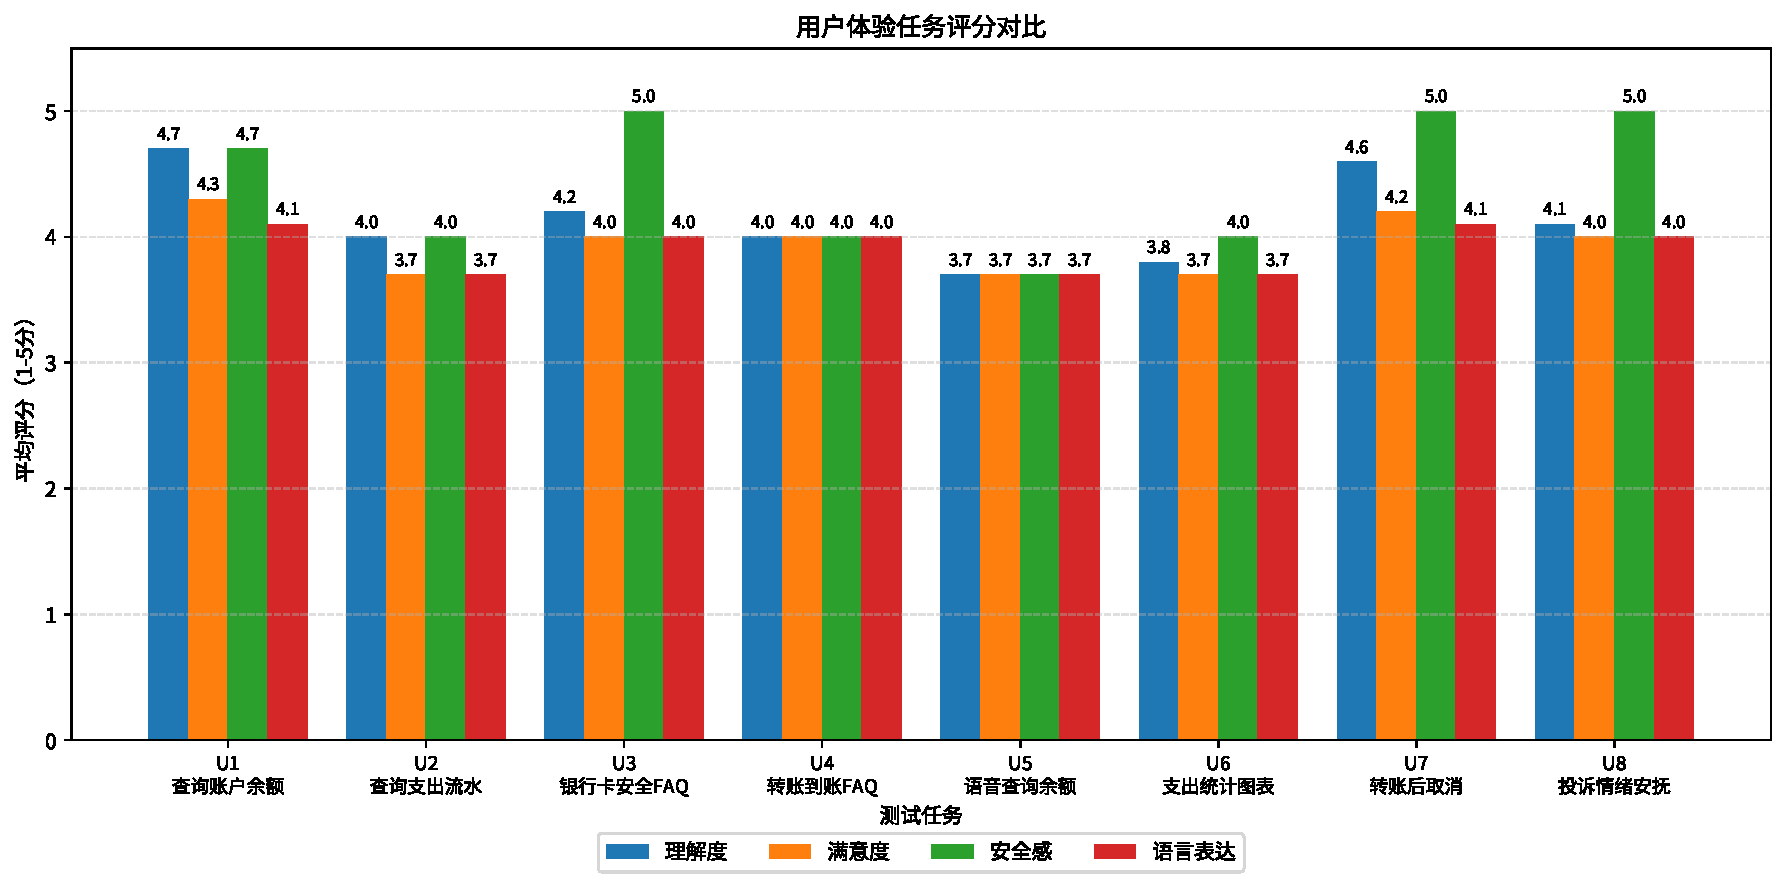
\includegraphics[width=0.92\linewidth]{image/fig_7_10_usability_scores_grouped_bar.pdf}
    \caption{用户体验任务评分对比}
    \label{fig:usability-scores-by-task}
\end{figure}

图 \ref{fig:usability-scores-by-task} 重点对比了不同用户体验任务的理解度、满意度、安全感和语言表达评分。余额查询、转账取消和投诉情绪安抚的评分较高，说明用户对查询类和安全确认类交互较容易理解。语音查询和支出统计图表的评分相对较低，反映出语音环境、权限提示、统计口径说明、图表解释和回复表达仍需要进一步优化。

\begin{figure}[H]
    \centering
    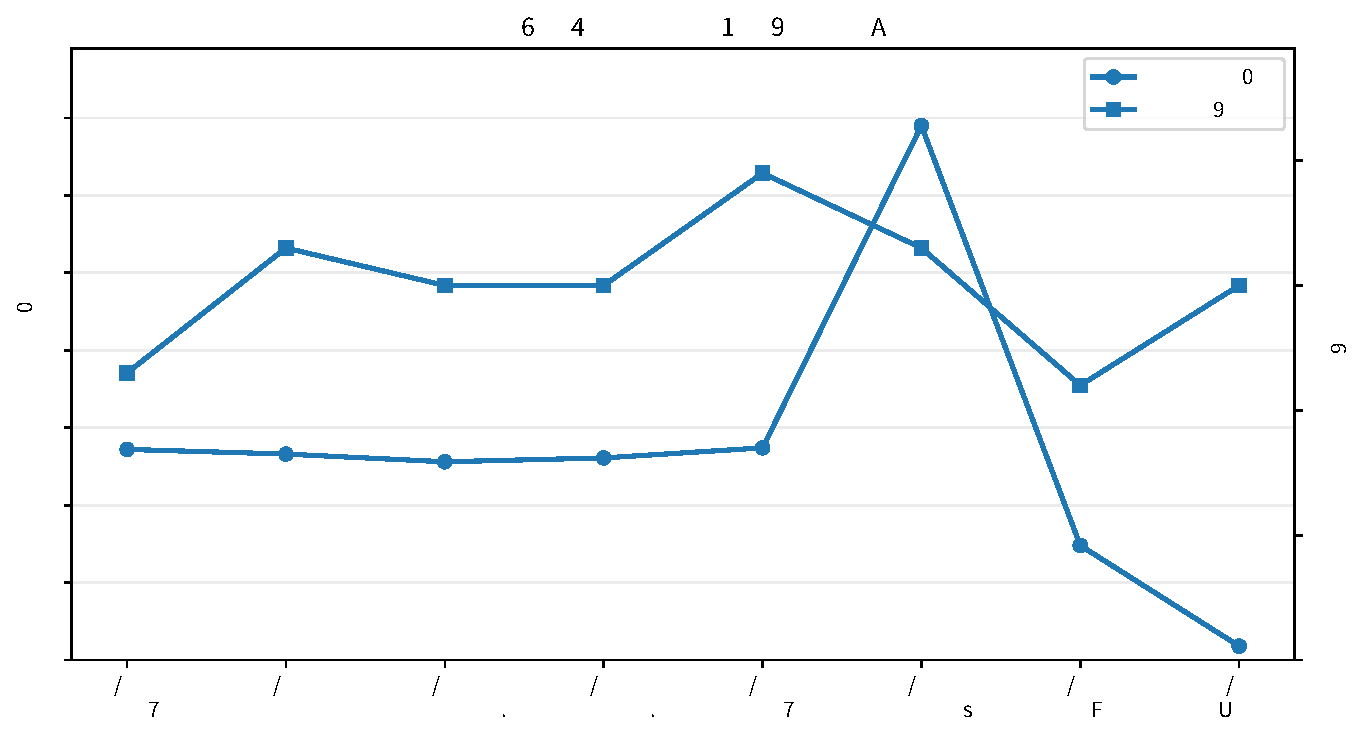
\includegraphics[width=0.92\linewidth]{image/fig_7_7_response_time_steps_trend.pdf}
    \caption{用户体验任务响应耗时与操作步数变化}
    \label{fig:response-time-steps-trend}
\end{figure}

图 \ref{fig:response-time-steps-trend} 展示了不同体验任务的平均响应耗时和平均操作步数变化。U6 支出统计图表的响应耗时明显高于其他任务，主要原因是该任务需要完成统计聚合、图表数据组织和说明文本生成。U7 转账取消和 U8 投诉情绪安抚耗时较低，说明规则分支和待确认状态处理具有较好的响应效率。结合表 \ref{tab:user-experience-summary} 可知，U2 支出流水查询虽能完成，但普通用户反馈中出现“筛选词不太会说”“希望默认突出支出”等意见，说明自然语言提示和结果展示还可以继续简化。

按测试对象类型汇总后的结果如表 \ref{tab:user-experience-role-summary} 所示。不同群体的评分差异与测试观察基本一致：计算机专业学生和开发者更关注状态流转与日志可追溯性，普通手机银行用户更关注是否容易说清需求、是否能看懂图表和语音输入是否稳定，行业导师更关注业务边界和安全说明。

\begin{table}[H]
    \centering
    \caption{不同测试对象的反馈汇总}
    \label{tab:user-experience-role-summary}
    \scriptsize
    \setlength{\tabcolsep}{2pt}
    \begin{tabular}{|p{0.2\linewidth}|p{0.08\linewidth}|p{0.09\linewidth}|p{0.09\linewidth}|p{0.09\linewidth}|p{0.09\linewidth}|p{0.24\linewidth}|}
        \hline
        用户群体 & 人数 & 聊天记录 & 满意度 & 安全感 & 语言 & 主要反馈 \\
        \hline
        计算机专业学生 & 3 & 27 & 4.1 & 4.6 & 4.1 & 流程顺畅，口语输入基本能命中，统计解释可再简化。 \\
        \hline
        普通手机银行用户 & 3 & 27 & 3.7 & 4.3 & 3.6 & 能完成主要操作，但语音权限、噪声和图表理解存在门槛。 \\
        \hline
        计算机行业开发者 & 2 & 18 & 4.0 & 4.6 & 4.0 & 状态流转、日志字段、FAQ 边界和取消链路较清楚。 \\
        \hline
        银行业务/企业导师 & 1 & 9 & 4.2 & 4.6 & 4.0 & 业务边界、风险提示和实验口径基本一致，建议强化口径说明。 \\
        \hline
    \end{tabular}
\end{table}

为了进一步回应“提高客户服务效率，减少人工客服负担”的目标，本文通过实际用户体验的使用反馈，将传统页面操作路径与 AI 助手操作路径进行对照。该对照不用于夸大系统性能数据，而是从页面跳转、筛选设置、人工咨询和确认步骤角度，说明智能客服入口对高频业务的路径压缩作用，结果如表 \ref{tab:efficiency-path-comparison} 所示。

\begin{table}[H]
    \centering
    \caption{传统页面操作与 AI 助手操作路径对照}
    \label{tab:efficiency-path-comparison}
    \scriptsize
    \setlength{\tabcolsep}{2pt}
    \begin{tabular}{|p{0.18\linewidth}|p{0.31\linewidth}|p{0.27\linewidth}|p{0.14\linewidth}|}
        \hline
        任务 & 传统页面操作 & AI 助手操作 & 优化效果 \\
        \hline
        查询最近 5 条支出流水 & 进入流水页，选择支出类型，设置时间或条数条件后查询。 & 输入“查最近 5 条支出记录”或相近口语表达。 & 操作步数减少。 \\
        \hline
        查询本月总支出 & 打开流水页，筛选本月支出记录，再查看图表或人工汇总。 & 输入“统计这个月总支出”，由后端生成统计和图表。 & 查询路径缩短。 \\
        \hline
        银行卡安全咨询 & 查找菜单、帮助文档或转人工客服咨询挂失、冻结等处理流程。 & 输入“卡丢了怎么办”等问题，由 FAQ 知识库返回标准答案或推荐。 & 常见问题直接回答。 \\
        \hline
        转账取消 & 进入转账页，填写收款人与金额信息后返回或取消。 & AI 生成确认信息后点击取消按钮。 & 降低误操作风险。 \\
        \hline
    \end{tabular}
\end{table}

从表 \ref{tab:efficiency-path-comparison} 可以看出，AI 助手并不是替代全部传统页面，而是在用户目标明确、操作路径较长或问题高频重复的场景中提供更短入口。对于流水查询和账单统计，系统将页面筛选条件转换为自然语言意图和后端查询参数；对于银行卡挂失等 FAQ 咨询，系统优先通过知识库回答，减少用户查找菜单或等待人工客服的可能；对于转账取消，系统把高风险操作停留在确认阶段，并提供取消按钮，使用户能够在执行前明确终止操作。因此，本文的效率提升主要体现在查询路径缩短、重复咨询分流和风险操作确认三个方面。

从反馈分析角度看，用户体验测试的价值不只在于得到评分，还在于将用户反馈转化为具体优化措施。结合 assistant\_test\_log 中的任务反馈和结束反馈，本文将主要反馈问题与对应优化措施整理如表 \ref{tab:user-feedback-optimization} 所示。

\begin{table}[H]
    \centering
    \caption{用户反馈问题与对应优化措施}
    \label{tab:user-feedback-optimization}
    \small
    \setlength{\tabcolsep}{4pt}
    \begin{tabular}{|p{0.38\linewidth}|p{0.52\linewidth}|}
        \hline
        用户反馈问题 & 对应优化措施 \\
        \hline
        普通用户不确定该如何描述支出筛选条件 & 在任务卡和快捷追问中增加“查最近 5 条支出”“本月支出汇总”等示例，引导用户使用更明确的表达。 \\
        \hline
        语音输入受浏览器权限、环境噪声和转写误差影响 & 保留语音转写后的文本确认步骤，并在语音失败时允许用户直接改为文字输入。 \\
        \hline
        统计图表需要配合文字解释才能理解 & 在图表上方增加统计口径、时间范围和总额说明，减少用户单独理解图表的成本。 \\
        \hline
        转账流程担心误操作 & 增加确认/取消按钮和账号脱敏展示，在用户明确确认前不执行扣款。 \\
        \hline
        常见业务问题不想查菜单 & 增加 FAQ 知识库问答，并通过 faq\_query\_log 记录未命中和推荐问题，便于后续补充知识库。 \\
        \hline
        投诉或焦虑问题不适合普通回答 & 增加情绪安抚和人工客服引导，避免系统继续输出普通闲聊式回答。 \\
        \hline
    \end{tabular}
\end{table}

匿名用户体验测试进一步观察用户是否能顺利理解和使用这些功能，从而使实验部分能够更完整地支撑本文的系统设计目标。

\section{交互优化设计分析}

第一，系统采用流式响应降低等待感。如\ref{fig:trace-ui}界面图展示，前端调用 /assistant/chat/stream 后，后端先返回 trace 事件，提示“请求已接收”和“正在识别业务意图”，最终再返回 message 事件。相比普通请求一次性返回结果，流式处理能让用户知道系统正在处理请求，减少等待过程中的不确定性。

第二，系统展示 AI 处理过程提升可解释性。如\ref{fig:trace-ui}界面图展示，AssistantChatResponse 中的 trace 字段包含 intent、tool、status、confidence 和 steps。前端将这些信息展示在聊天气泡中，使用户和答辩评阅者能够看到系统识别了什么意图、调用了什么能力以及处理状态。

第三，系统通过图表增强统计结果表达。如\ref{fig:statistics-ui}界面图展示，对于趋势类统计，用户不仅能看到文字总结，还能看到柱状图或折线图。对于收支概览，系统能够展示收支对比和按对方账号聚合的饼图。图表展示降低了用户理解复杂流水数据的成本。

第四，系统提供语音输入减少文字输入成本。用户点击语音输入按钮后可以直接说出查询或转账需求，前端将语音识别结果填入输入框。该设计对演示场景较为直观，也使语音识别要求落到实际交互功能中。

第五，系统提供情绪安抚与人工客服引导。对于明显包含投诉、焦虑或愤怒的输入，系统不直接进入普通闲聊，而是先返回安抚性说明，并提示用户拨打虚拟客服电话 010-1234-5678 联系人工客服。该设计使智能客服在处理业务查询之外，也具备基本的客服分流意识。

第六，系统提供 FAQ 知识库问答。对于银行卡挂失、密码找回、转账到账时间等常见咨询问题，系统优先从数据库知识库返回标准答案；若没有达到直接命中阈值，则根据匹配得分给出相似问题并提示用户进一步提问，同时记录查询日志，便于后续分析用户高频问题和未收录问题。

第七，系统提供快捷操作减少输入成本。简报卡片提供快捷追问按钮，用户可以一键继续查询；转账确认场景中显示“确认”和“取消”按钮，减少用户手动输入。

第八，系统对不支持能力进行边界控制。当前项目并未实现消费品类、商户类型和场景标签分析，因此后端在意图解析后会对这些需求进行拦截，避免大模型给出超出系统能力的结论。这种设计有利于提高银行场景下的可信度。

\begin{figure}[H]
    \centering
    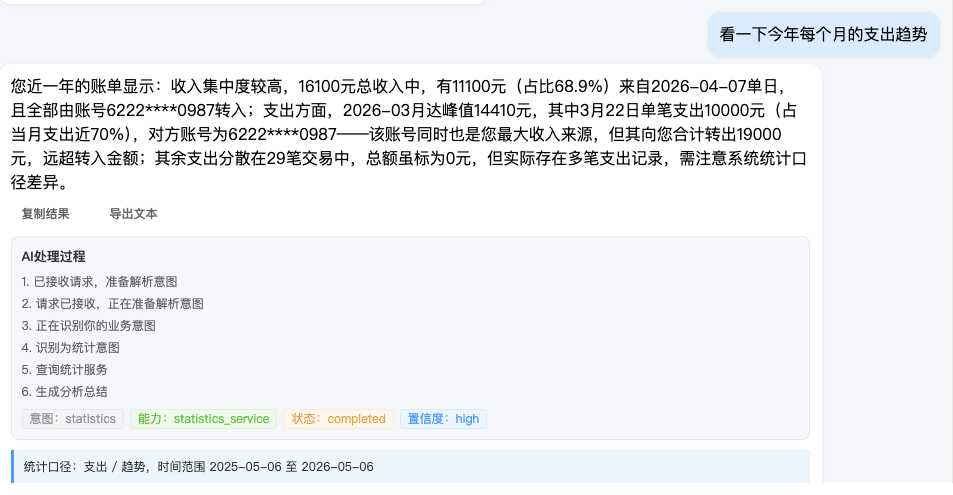
\includegraphics[width=0.95\linewidth]{image/fig-trace-ui.png}
    \caption{AI 处理过程展示界面图}
    \label{fig:trace-ui}
\end{figure}

\begin{figure}[H]
    \centering
    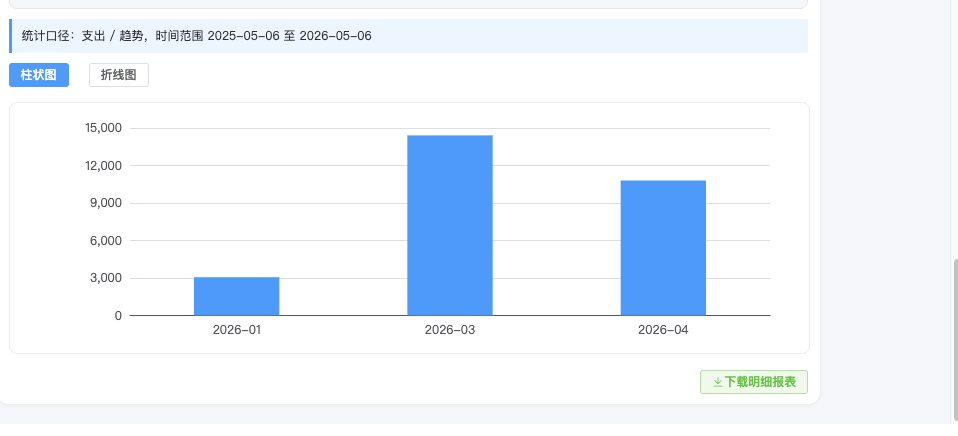
\includegraphics[width=0.95\linewidth]{image/fig-statistics-ui.png}
    \caption{AI 统计图表展示界面图}
    \label{fig:statistics-ui}
\end{figure}

\section{测试结论}

综合功能测试和交互分析，BankCopilot 智能客服机器人能够较好地完成文本输入和语音转文字输入形式的银行业务交互。系统在查询类任务中能够正确调用账户和流水服务，在统计类任务中能够基于数据库聚合结果生成图表和分析，在 FAQ 咨询中能够从知识库返回标准答案或相似问题推荐，在转账类任务中能够通过二次确认保证资金操作安全。虽然目前系统核心功能较少，但其链路完整，涉及场景典型，整体设计体现了智能客服机器人在银行场景中的可行性和实用价值。

从测试结论看，本文系统已经完成了从自然语言输入到业务服务调用、知识库检索、再到结构化结果展示的闭环。其主要优势体现在三个方面：第一，系统没有把银行业务结果和常见问题答案完全交给大模型生成，而是以真实数据库、知识库表和后端服务为依据；第二，系统对查询、统计、FAQ 和转账采用不同交互策略，能够根据业务风险调整流程复杂度；第三，系统在展示层面保留 AI 处理过程和统计口径说明，便于用户理解系统为何给出某一结果。

同时，受项目周期、原型系统定位和企业业务数据保密要求限制，本文测试未接入真实银行生产数据，也未覆盖真实银行系统中的复杂账户状态、异常交易、并发转账和风控规则。测试数据规模较小，FAQ 知识库条目数量有限，自动化测试主要覆盖服务层核心分支，尚不能覆盖真实银行系统中复杂的账户状态、异常交易、并发转账和风控规则。如果将系统扩展到更真实的业务环境，还需要继续补充接口集成测试、压力测试、安全测试和异常恢复测试。本文在结论中将这些问题作为不足进行说明，避免夸大系统当前能力。

\chapter{结论与展望}

\section{主要结论}

本文围绕“智能客服机器人的设计与交互优化”这一课题，完成了 BankCopilot 银行智能客服机器人原型的设计与实现。作为本科计算机专业毕业设计，本系统的定位不是构建完整商业银行系统，而是在一个规模可控的银行管理系统中，验证 AI 能力如何与传统业务管理系统结合。系统整体功能不追求大而全，而是围绕语音输入、FAQ 知识库问答、异常情绪安抚、余额查询、流水查询、账单统计、周报/月报和智能转账等典型场景，形成一个小而完整、边界清晰、能够演示的 AI 业务闭环。

从功能设计看，各项 AI 能力承担的业务角色并不重复。AI 语音输入主要体现自然语言输入方式的扩展，用户可以通过语音说出需求，再由前端转写为文本进入同一聊天链路。FAQ 知识库问答主要处理银行卡挂失、转账到账时间、密码找回等常见咨询，答案来自数据库知识库表。AI 情绪安抚主要体现客服场景中的异常情绪关键词检测和人工客服引导，系统识别明显负面情绪后返回安抚话术和虚拟客服电话。AI 查余额主要体现自然语言到数据库单对象查询的转换，用户用口语化方式提出问题，后端仍然从账户表读取真实余额和账户状态。AI 查流水体现自然语言条件到列表查询条件的转换，系统需要识别交易方向、条数限制和时间范围。AI 账单统计与分析体现数据库聚合能力，系统将流水数据进一步转换为总额、笔数、趋势和对比结果。AI 周报/月报是在统计结果基础上的概览展示，强调主动汇总和快捷追问。AI 智能转账则对应传统管理系统中最典型的流程型操作，需要按照收款人匹配、金额解析、业务校验、待确认、确认执行或取消的步骤逐步完成。

从系统实现看，AI 与传统管理系统结合时，关键不在于让模型直接完成所有业务，而在于明确模型和后端系统的职责边界。大语言模型适合完成自然语言理解、意图识别和结果表达，但账户数据、流水数据、统计结果和转账执行必须由 Spring Boot 后端和 MySQL 数据库提供确定性支持。对于银行业务这类需要准确性和可追溯性的场景，时间范围、统计指标、交易方向、金额、收款人和确认状态等条件都必须被明确约束，不能由模型自由推断。

从论文创新性看，BankCopilot 的创新不在于提出新的大模型算法，而在于围绕银行业务原型完成系统设计和工程集成创新。第一，系统面向银行高频业务构建自然语言辅助操作流程，将余额查询、流水查询、账单统计、FAQ 咨询和转账确认统一接入 AI 助手，使传统页面操作扩展为文本和语音转文字驱动的智能交互。第二，系统设计了大语言模型与确定性业务服务分离的集成方式，大模型只负责意图解析和分析性表达，账户、流水、统计和转账结果均由后端服务和数据库生成，从而降低模型幻觉对业务事实的影响。第三，系统围绕银行业务安全和用户理解成本，引入处理过程展示、统计口径说明、FAQ 日志、异常情绪分流、转账二次确认、取消回退和历史金额复用等机制，使智能客服具备可解释、可控制和可验证的业务辅助能力。

\section{实践价值}

BankCopilot 的实践价值主要体现在智能客服能力与银行业务流程的结合。传统页面更适合结构化操作，但当用户目标明确而路径复杂时，自然语言入口可以减少页面查找和条件设置成本。例如，用户只需要输入“查最近 5 条支出记录”，系统即可完成意图识别、条件转换、流水查询和结果展示。对于账单统计，系统能够把分散流水转化为总额、趋势和概览，使用户更容易理解账户变化。

在安全性方面，本文系统没有因为引入 AI 而弱化业务控制。尤其在转账功能中，系统把自然语言解析结果转化为待确认信息，并在确认前保持状态而不执行资金变动。这种方式既保留了智能交互的便利性，又符合资金类业务需要用户明确授权的原则。对于毕业设计展示而言，该功能能够较直观地体现“智能”并不等同于自动越权执行，而是要在用户授权、业务规则和交互体验之间取得平衡。

在可解释性方面，系统通过 trace 信息展示意图、工具、状态、置信度和处理步骤。该设计使 AI 处理过程从黑盒回复变为可观察链路，便于用户理解系统处理逻辑，也便于教师在评阅时确认系统不是简单静态问答。对于账单分析和统计图表，系统同时给出统计口径说明，避免用户把不同时间范围、不同交易方向或不同聚合方式下的结果混淆。

\section{不足与展望}

受本人开发经验、项目周期和测试条件限制，当前系统仍然存在一些不足。首先，多轮对话状态主要保存在后端内存中，服务重启后会丢失，这种方式适合毕业设计原型展示，但距离长期稳定运行还有差距。其次，系统依赖外部大模型服务，当网络异常或模型接口不可用时，意图解析和分析总结能力会受到影响，虽然已有部分规则化后备处理，但还不够完善。再次，当前交易流水数据字段较简单，系统能够完成余额查询、流水查询、统计分析和转账确认，但还不能深入分析消费品类、商户类型和具体消费场景。

如果后续有机会继续完善该系统，我认为可以从几个较实际的方向改进。第一，可以将待确认转账、待补全查询等会话状态保存到 Redis 或数据库中，提高系统重启后的恢复能力。第二，可以继续补充异常情况处理和测试用例，例如模型返回格式异常、网络请求失败、余额不足、收款人不存在等场景，使系统在演示之外更加稳定。第三，可以在交易流水中增加更丰富的字段，并在此基础上扩展消费分类、预算提醒和更细粒度的账单分析功能。通过这些改进，BankCopilot 可以在现有毕业设计原型的基础上进一步完善，但就本次毕业设计而言，系统已经完成了 AI 与传统银行管理系统结合的主要设计目标。

\chapter{结束语}

本文围绕个人银行业务中的智能客服交互问题，完成了从需求分析、总体设计、核心功能实现到测试分析的完整论述。论文写作过程中始终以本人独自完成的项目源码为依据，只对系统中已经实现并能够演示的功能进行说明，没有将未完成的功能写入系统成果。系统的重点不是构建一个泛化聊天机器人，而是在一个具体的银行管理系统中，验证大语言模型与确定性业务服务结合的实现方式。

从实现结果看，BankCopilot 已经能够处理语音输入、FAQ 知识库问答、异常情绪安抚、余额查询、流水查询、账单统计、周报/月报和智能转账等典型场景。系统通过语音转文字和自然语言意图识别降低用户操作门槛，通过数据库知识库提供常见问题标准答案，通过规则化情绪检测补充客服安抚与人工引导，通过后端业务服务保证数据来源和资金操作的确定性，通过处理过程展示、统计口径说明和转账二次确认增强交互可解释性与可控性。虽然该系统仍然存在测试数据规模有限、风控规则较简单、会话状态未持久化等不足，但作为本科毕业设计原型，已经较完整地展示了 AI 能力嵌入传统管理系统后的基本流程和实现效果。

通过本课题的完成，本人对前后端分离开发、数据库建模、接口设计、自然语言意图识别、流式交互和 LaTeX 论文写作有了更系统的认识。整个开发和论文整理过程也让我认识到，AI 功能落地到具体业务系统时，不能只关注模型回复是否自然，更需要关注数据来源、业务约束、异常处理和用户确认等工程细节。本次毕业设计仍有不足，但基本达到了任务书对系统设计、功能实现和论文撰写的要求。

\chapter*{致谢}

本论文和系统原型的完成离不开指导教师和企业专家导师在选题方向、系统设计和论文写作方面的指导。在项目实现过程中，相关课程学习和开源技术文档为系统架构设计、前后端开发和数据库实现提供了重要帮助。同时，感谢在毕业设计过程中给予建议和支持的指导教师、企业专家导师，辅导员和同学。由于本人能力和时间有限，论文和系统仍存在不足之处，恳请各位批阅老师批评指正。

\bibliographystyle{gbt7714-numerical}
\bibliography{ref}

\begin{appendix}

\chapter{主要接口与数据结构}

\section{AI 聊天请求结构}

AI 聊天请求由 AssistantChatRequest 承载，核心字段为 message。用户自然语言输入会以 JSON 请求体形式发送至 /assistant/chat 或 /assistant/chat/stream 接口。

\begin{table}[H]
    \centering
    \caption{AssistantChatRequest 请求字段}
    \label{tab:assistant-request}
    \begin{tabular}{|p{0.2\linewidth}|p{0.2\linewidth}|p{0.5\linewidth}|}
        \hline
        字段 & 类型 & 说明 \\
        \hline
        message & String & 用户自然语言输入，例如“统计这个月总支出”。 \\
        \hline
    \end{tabular}
\end{table}

\section{AI 聊天响应结构}

\begin{table}[H]
    \centering
    \caption{AssistantChatResponse 响应字段}
    \label{tab:assistant-response}
    \begin{tabular}{|p{0.2\linewidth}|p{0.2\linewidth}|p{0.5\linewidth}|}
        \hline
        字段 & 类型 & 说明 \\
        \hline
        reply & String & AI 回复文本。 \\
        \hline
        chartType & String & 图表类型，如 number、bar、line、overview。 \\
        \hline
        chartData & Object & 图表数据或数字统计结果。 \\
        \hline
        exportUrl & String & 导出交易流水的链接。 \\
        \hline
        trace & TraceInfo & AI 处理过程信息。 \\
        \hline
        explain & Map & 查询或统计口径说明。 \\
        \hline
    \end{tabular}
\end{table}

\section{统计查询结构}

\begin{table}[H]
    \centering
    \caption{StatisticsQueryDTO 字段说明}
    \label{tab:statistics-query}
    \begin{tabular}{|p{0.25\linewidth}|p{0.65\linewidth}|}
        \hline
        字段 & 说明 \\
        \hline
        accountId & 账户 ID。 \\
        \hline
        txnType & 收入或支出。 \\
        \hline
        metric & 统计指标，支持 sum、count、max、trend。 \\
        \hline
        groupBy & 分组方式，支持 none、day、month。 \\
        \hline
        startTime & 统计开始时间。 \\
        \hline
        endTime & 统计结束时间。 \\
        \hline
        rangeValue & 最近 N 天或 N 年的数值。 \\
        \hline
        comparePrevious & 是否对比上一周期。 \\
        \hline
    \end{tabular}
\end{table}


\section{测试样本说明}
\label{app:test-samples}

为避免将少量功能用例误写成开放域测试，本文在附录中补充意图识别和 FAQ 知识库测试样本的构成说明。意图与分流测试样本围绕系统已经实现的基础意图类型和服务编排分支设计，每类 10 条，共 80 条，样本构成如表 \ref{tab:intent-sample-appendix} 所示。

\begin{table}[H]
    \centering
    \caption{意图与分流测试样本构成}
    \label{tab:intent-sample-appendix}
    \small
    \setlength{\tabcolsep}{4pt}
    \begin{tabular}{|p{0.22\linewidth}|p{0.14\linewidth}|p{0.54\linewidth}|}
        \hline
        测试类型 & 样本数量 & 典型样例 \\
        \hline
        balance 基础意图 & 10 & 查一下我的余额；我现在账户里还有多少钱。 \\
        \hline
        transactions 基础意图 & 10 & 查最近 5 条支出记录；17 号收入记录给我看看。 \\
        \hline
        statistics 基础意图 & 10 & 统计这个月总支出；最近 7 天支出趋势。 \\
        \hline
        transfer 基础意图 & 10 & 给弟弟转 300 元午餐费；给弟弟转晚餐费，和昨天一样。 \\
        \hline
        FAQ 咨询分流 & 10 & 卡丢了怎么挂失；跨行转账要多久；验证码收不到怎么办。 \\
        \hline
        情绪关键词后备处理 & 10 & 我很生气，我要投诉；我有点担心这笔钱；服务太差了。 \\
        \hline
        不支持能力拦截 & 10 & 按消费场景标签统计一下；按商户类型分析消费；给我推荐理财产品。 \\
        \hline
        多轮与确认状态 & 10 & 1月；确认；取消；不转了；重新查今年1月收入。 \\
        \hline
    \end{tabular}
\end{table}

FAQ 知识库测试样本来自项目中的 \texttt{sql/faq\_test\_dataset.csv}，覆盖标准 FAQ 相似问法、模糊问法和无关问题三类，共 60 条，样本构成如表 \ref{tab:faq-sample-appendix} 所示。第七章统计表从该数据集中选取 50 条按业务类别重新分组统计。

\begin{table}[H]
    \centering
    \caption{FAQ 知识库测试样本构成}
    \label{tab:faq-sample-appendix}
    \small
    \setlength{\tabcolsep}{4pt}
    \begin{tabular}{|p{0.2\linewidth}|p{0.14\linewidth}|p{0.24\linewidth}|p{0.32\linewidth}|}
        \hline
        样本类型 & 数量 & 期望结果 & 典型样例 \\
        \hline
        标准 FAQ 相似问法 & 40 & hit & 卡丢了怎么挂失；跨行转账要多久；短信验证码不来。 \\
        \hline
        模糊问法 & 10 & recommend & 转账有问题；密码怎么办；贷款怎么办。 \\
        \hline
        无关或未收录问题 & 10 & no\_answer & 今天上海天气怎么样；帮我订一张机票；写一首诗。 \\
        \hline
    \end{tabular}
\end{table}

\section{匿名反馈测试日志明细}
\label{app:usability-log-details}

本附录补充第七章用户体验测试的数据来源说明。匿名反馈测试记录保存在 assistant\_test\_log 表中，source 字段取值为 usability\_live。测试时间范围为 2026 年 4 月 21 日 12:40:00 至 2026 年 4 月 29 日 10:13:30。该数据由测试者在本地原型环境中完成匿名反馈测试后形成，账户、流水和转账对象均为系统演示数据，不包含真实银行客户生产数据。

\begin{table}[H]
    \centering
    \caption{匿名反馈测试日志记录类型}
    \label{tab:usability-log-scenario-appendix}
    \small
    \setlength{\tabcolsep}{4pt}
    \begin{tabular}{|p{0.24\linewidth}|p{0.16\linewidth}|p{0.5\linewidth}|}
        \hline
        场景类型 & 记录数 & 说明 \\
        \hline
        feedback\_session\_start & 9 & 记录测试开始时间、匿名角色、participant\_code 和 test\_session\_id。 \\
        \hline
        assistant\_chat\_test & 81 & 记录 U1--U8 任务中的用户原始输入、系统识别意图、调用工具、响应耗时、操作步数、四类评分和任务反馈。 \\
        \hline
        feedback\_session\_end & 9 & 记录测试结束时间和测试者对整个匿名反馈测试过程的总结性反馈。 \\
        \hline
    \end{tabular}
\end{table}

\begin{table}[H]
    \centering
    \caption{匿名反馈测试对象明细汇总}
    \label{tab:usability-participant-appendix}
    \scriptsize
    \setlength{\tabcolsep}{2pt}
    \begin{tabular}{|p{0.06\linewidth}|p{0.16\linewidth}|p{0.08\linewidth}|p{0.08\linewidth}|p{0.08\linewidth}|p{0.08\linewidth}|p{0.08\linewidth}|p{0.28\linewidth}|}
        \hline
        编号 & 分组 & 聊天记录 & 任务数 & 响应/s & 满意度 & 安全感 & 结束反馈摘要 \\
        \hline
        P1 & 计算机专业学生 & 9 & 8 & 2.34 & 4.2 & 4.6 & 流程顺，转账前确认和取消让用户有底。 \\
        \hline
        P2 & 计算机专业学生 & 9 & 8 & 2.40 & 4.0 & 4.6 & 口语输入基本能命中，统计解释还能再短一点。 \\
        \hline
        P3 & 计算机专业学生 & 9 & 8 & 2.53 & 4.2 & 4.6 & 查询与投诉引导在线，语音入口比较好找。 \\
        \hline
        P4 & 普通手机银行用户 & 9 & 8 & 2.73 & 3.7 & 4.3 & 能完成主要操作，但模糊问法下需要更直白提示。 \\
        \hline
        P5 & 普通手机银行用户 & 9 & 8 & 2.91 & 3.7 & 4.3 & 语音权限和图表理解有门槛，文字总结更关键。 \\
        \hline
        P6 & 普通手机银行用户 & 9 & 8 & 3.00 & 3.7 & 4.3 & 噪声环境下语音容易偏，其他流程基本可完成。 \\
        \hline
        P7 & 计算机行业开发者 & 9 & 8 & 2.37 & 4.0 & 4.6 & 状态流转、日志字段和取消链路清晰，可用于排查。 \\
        \hline
        P8 & 计算机行业开发者 & 9 & 8 & 2.45 & 4.0 & 4.6 & 查询与转账确认链路稳定，FAQ 边界表达合理。 \\
        \hline
        P9 & 银行业务/企业导师 & 9 & 8 & 2.61 & 4.2 & 4.6 & 业务边界、风险提示与论文实验口径一致，建议继续强化口径说明。 \\
        \hline
    \end{tabular}
\end{table}

\begin{table}[H]
    \centering
    \caption{匿名反馈测试原始输入与反馈节选（3轮U1--U8）}
    \label{tab:usability-query-feedback-appendix}
    \scriptsize
    \setlength{\tabcolsep}{2pt}
    \begin{tabular}{|p{0.06\linewidth}|p{0.06\linewidth}|p{0.32\linewidth}|p{0.44\linewidth}|}
        \hline
        编号 & 任务 & 原始输入 & 任务反馈 \\
        \hline
        P1 & U1 & 兄弟，帮我瞅一眼卡里还剩多少钱 & 余额结果直给，像平时查卡余额一样顺手。 \\
        \hline
        P1 & U2 & 把我最近花出去的5笔甩出来 & 能看懂，但要是默认突出支出会更省脑子。 \\
        \hline
        P1 & U3 & 卡可能丢了，我先干啥，挂失还是冻结 & FAQ 能先给步骤，再补风险说明，顺序对。 \\
        \hline
        P1 & U4 & 今晚跨行转账，最晚啥时候到 & 到账时效讲得比较稳，没有乱承诺。 \\
        \hline
        P1 & U5 & 语音输入：我卡里还剩多少 & 语音转文字后还能命中余额查询。 \\
        \hline
        P1 & U6 & 本月我花了多少，顺便给个图 & 总额和图能对应上，解释再多一句更好。 \\
        \hline
        P1 & U7 & 给弟弟转300，备注午饭 & 先弹确认再转账，这点很稳。 \\
        \hline
        P1 & U7 & 算了先撤销这笔 & 取消提示明确，没有真实扣款风险。 \\
        \hline
        P1 & U8 & 这回答让我有点上头，我要投诉 & 先安抚再引导人工，节奏没问题。 \\
        \hline
        P4 & U1 & 我想看看账户里钱还够不够 & 能查到余额，但我得看两遍才反应过来。 \\
        \hline
        P4 & U2 & 最近花的钱大概啥情况，给我看下 & 我说得比较模糊，系统还能给出结果。 \\
        \hline
        P4 & U3 & 银行卡找不到了我该先做哪一步 & 先挂失再处理的提示让我安心。 \\
        \hline
        P4 & U4 & 跨行转账一般什么时候能到呀 & 时间说法比较日常，我能理解。 \\
        \hline
        P4 & U5 & 语音输入：我这个账户还有钱吗 & 语音能用，但有时要重新说一遍。 \\
        \hline
        P4 & U6 & 这个月总共花了多少钱，图也看一下 & 图表有帮助，不过解释再简单点更好。 \\
        \hline
        P4 & U7 & 给弟弟转三百块午饭钱 & 先确认再执行，这一步很必要。 \\
        \hline
        P4 & U7 & 先别转了，取消掉 & 取消后我比较放心。 \\
        \hline
        P4 & U8 & 我有点生气，想找人工客服 & 情绪场景有安抚，不会继续答非所问。 \\
        \hline
        P7 & U1 & 查询 demo\_account 可用余额，返回金额与更新时间 & 返回字段稳定，余额来源可追溯。 \\
        \hline
        P7 & U2 & 按 direction=OUT 查询最近5条交易，按时间倒序 & 排序和方向过滤符合预期。 \\
        \hline
        P7 & U3 & 银行卡遗失场景，请返回挂失与冻结的处理顺序 & 知识库命中准确，动作顺序可执行。 \\
        \hline
        P7 & U4 & 说明跨行转账 T+0/T+1 到账条件 & FAQ 对边界条件描述清楚。 \\
        \hline
        P7 & U5 & 语音输入：查询当前可用余额 & 语音只影响输入层，后端链路一致。 \\
        \hline
        P7 & U6 & 统计本月支出并返回图表数据与口径 & 统计数值与图表一致，可复核。 \\
        \hline
        P7 & U7 & 发起向弟弟转账300元，验证待确认状态 & transfer\_validation 状态流转正确。 \\
        \hline
        P7 & U7 & 取消待确认转账 & 取消后 pending 状态清理正确。 \\
        \hline
        P7 & U8 & 模拟投诉：回答不满意，请转人工 & emotion\_support 分流规则可预期。 \\
        \hline
    \end{tabular}
\end{table}

\end{appendix}

\end{document}
